\documentclass[answers]{exam}
% 'texPreamble' contains formatting and macros. 
% https://github.com/pwesterbaan/scripts/tree/master/texmf/tex/latex/local
\usepackage{texPreamble}
\usepackage{relsize}
\usepackage{tkz-euclide}
\usepackage[titles]{tocloft}
\renewcommand{\cftsecleader}{\cftdotfill{\cftdotsep}}
\usetkzobj{all}
%% Externalize graphics and save in ./images/ folder
%% pdflatex -shell-escape <tex file>
%% The document can be compiled with the two following
%% lines commented out, but will recompile all figures
%% each time.
\usetikzlibrary{external}
\tikzexternalize[prefix=images/]
%% 
\usepackage{tabularx}
\extraheadheight{0.25in}
\extrafootheight{1.0in}
\extrawidth{1in}
% ----------------------------------------------------------------
\makeatletter
\title{Math 1070 Class notes\\[0.25\baselineskip]Spring 2020}
\author{\thefname\ \thelname}

\pagestyle{headandfoot}

%\firstpageheader{\@title\\\@date}{}{Math 1070}
%\firstpageheadrule

\newcommand*{\currentname}{\@currentlabelname}

\runningfootrule
\runningfooter{\parbox{0.45\linewidth}{\currentname}}{\thepage}{\@title}
\makeatother

\begin{document}
  %% Title
  \pagenumbering{roman}
  \vspace*{\stretch{1}}
  \begin{center}
    \makeatletter
    {\huge
    \@title}\\[\baselineskip]
    \@author\\[\baselineskip]
    Last updated:
    \@date\\
    \makeatother
  \end{center}
  \vspace*{\stretch{1}}
  \thispagestyle{empty}
  \pagebreak
  \pagestyle{headandfoot}

  \renewcommand{\contentsname}{Table Of Contents}
  \renewcommand\thesection{}
  \tableofcontents
  \newpage
  
  \makeatletter
  \firstpageheader{}{}{}
  \firstpagefooter{\parbox{0.45\linewidth}{\currentname}}{\thepage}{\@title}
  \firstpagefootrule
  \makeatother
  \pagenumbering{arabic}
  \setcounter{page}{1}
  %% everything else
  \relscale{1.4}

\documentclass[mathNotesPreamble]{subfiles}
\begin{document}
%\relscale{1.4} %TODO
\section{MATH 1040 Review}
  For the following functions, find their derivatives:
  \begin{tasks}[after-item-skip=\stretch{0.5}, label=](2)
    \task $y=\sqrt[7]{x^3}-\pi e^x+x^e+3e\inv[x]$
    \task $f(x)=\parens{\frac{1-\sin(x)}{1+\cos(x)}}$
    \task $g(x)=\parens{\frac{x^2+3x+1}{e^x}}$
    \task $h(y)=-5\cot\parens{3e^{4y}}+e^\pi$
  \end{tasks}
  \vspace*{\stretch{0.5}}
  Find $f''(x)$ for $f(x)=\tan(x)$
  \vspace*{\stretch{1}}
  \pagebreak
  
  Find the equation of the line tangent to $\ell(x)=x\sqrt{5-x^2}$ at the point $(1,2)$.
  \vspace*{\stretch{1}}
  
  Where is the tangent line of $u=\dfrac{1}{\sqrt x}$ parallel to the line $y=-4x-3$?
  \vspace*{\stretch{1}}
  \pagebreak

  %% 01/14/19
  \noindent
  \textbf{Note:} Limits will be on Test 1 and the final exam.
  \begin{ex*}~

  Using the graph below, evaluate each limit:
  \end{ex*}
  
  \begin{minipage}{0.275\linewidth}
    \begin{tikzpicture}
      \begin{axis}[
        axis lines=center,
        axis line style={->},
        xmin=-1.5, xmax=2.25, 
        ymin=-0.5, ymax=1.5,
        xtick={-6,-5,...,6},
        ytick={-6,-5,...,6},
        ticklabel style={font=\footnotesize,inner sep=0.5pt,fill=white,opacity=1.0, text opacity=1},
        height=0.95*2.0in, width=0.75*3.75in,
        xlabel=$x$, xlabel style={at={(ticklabel* cs:1)},anchor=north west},
        ylabel=$y$, ylabel style={at={(ticklabel* cs:1)},anchor=south west},
        every axis plot/.append style={line width=0.95pt}
        ]
        \addplot[-] expression[domain=-1:1, blue]{x^2};
        \node[anchor=south west] at(axis cs: 0.85,1.05) {$y=f(x)$};
        \addplot[-] expression[domain=1:2, blue]{0};
        \addplot[soldot] coordinates{(-1,1)(0,1)(1,0)(2,0)};
        \addplot[holdot] coordinates{(0,0)(1,1)};
      \end{axis}
    \end{tikzpicture}
  \end{minipage}%
  \begin{minipage}{0.725\linewidth}
    \begin{tasks}[after-item-skip=20pt,label=](3)
      \task $\ds\lim_{x\to -1^+} f(x)$
      \task* $\ds\lim_{x\to 2^-} f(x)$
      \task $\ds\lim_{x\to 0^-} f(x)$
      \task $\ds\lim_{x\to 0^+} f(x)$
      \task $\ds\lim_{x\to 0} f(x)$
      \task $\ds\lim_{x\to 1^-} f(x)$
      \task $\ds\lim_{x\to 1^+} f(x)$
      \task $\ds\lim_{x\to 1} f(x)$
    \end{tasks}
  \end{minipage}
  
  \vspace*{15pt}
  State the intervals of continuity on $[-1,2]$.
  \vspace*{\stretch{0.5}}
  \begin{ex*}
    Algebraically, evaluate the following limits
  \end{ex*}
  \begin{tasks}[after-item-skip=\stretch{1}, label=](2)
    \task $\ds\lim_{x\to 0}\parens{\sin^2 x+\sec x}$
    \task $\ds\lim_{y\to 0}\frac{5y^3+8y^2}{3y^4-16y^2}$
  \end{tasks}
  \vspace*{\stretch{1}}
  \pagebreak
  
  \begin{tasks}[after-item-skip=\stretch{1}, label=](2)
    \task $\ds\lim_{x\to \frac{1}{2}^-} \frac{4x-2}{\abs{2x^3-x^2}}$
    \task $\ds\lim_{x\to 0} \frac{1-\cos x}{\cos^2 x-3\cos x+2}$
    \task $\ds\lim_{x\to 0} \frac{x}{\sqrt{5x+1}-1}$
    \task $\ds\lim_{x\to 0} \frac{e^{4x}-1}{e^{x}-1}$
    \task $\ds\lim_{x\to 0} \frac{\sin(x)}{x}$
    \task $\ds\lim_{x\to 0} \frac{\tan(3x)}{5x}$
  \end{tasks}
  \vspace*{\stretch{1}}
  \pagebreak
  
  \begin{tasks}[after-item-skip=\stretch{1}, label=](2)
    \task $\ds\lim_{x\to \infty} \frac{4x^3+1}{2x^3+\sqrt{16x^6+1}}$
    \task $\ds\lim_{x\to -\infty} \frac{4x^3+1}{2x^3+\sqrt{16x^6+1}}$
    \task $\ds\lim_{x\to -\infty} \parens{x+\sqrt{x^2+2x}}$
  \end{tasks}
  \vspace*{\stretch{1}}
  \pagebreak
  
  \begin{tasks}[after-item-skip=\stretch{1}, label=](2)
    \task $\ds\lim_{t\to -2^-} \frac{t^3-5t^2+6t}{t^4-4t^2}$
    \task $\ds\lim_{t\to -2^+} \frac{t^3-5t^2+6t}{t^4-4t^2}$
    \task $\ds\lim_{x\to -\infty} \frac{3x+7}{x^2-4}$
  \end{tasks}
  \vspace*{\stretch{1}}
  \pagebreak
  
  Find the equation of the slant (oblique) asymptote of $\ds f(x)=\frac{3x^5+x^4+2x^2+1}{x^4+3}$.
  \pagebreak
  
  Find $k$ such that $f(x)$ is continuous at $x=1$:
    $$f(x)=\begin{cases}
      k\,\tan\parens{\frac{\pi x}{3}},& x\geq 1\\
      x-2,& x<1
    \end{cases}$$
  \vspace{\stretch{1}}
  
  Find $c$ such that $f(x)$ is continuous:
    $$f(x)=\begin{cases}
      \dfrac{\sin^2 3x}{x^2},& x\neq 0\\
      c,& x=0
    \end{cases}$$
  \vspace*{\stretch{1}}
  \pagebreak 
  
\textbf{$\delta \textnormal{ --- } \eps$ proofs:}

  \begin{center}
    \begin{tikzpicture}[scale=0.825]
      \begin{groupplot}[
        group style={group size=3 by 1},
        axis lines=center,
        axis line style={->},
        xmin=0, xmax=4,
        ymin=0, ymax=4,
        enlargelimits={abs=0.65},
        ticklabel style={font=\large, inner sep=0.75pt,fill=white},
	      every axis plot/.append style={line width=0.95pt}
        ]
        \nextgroupplot[xtick={2.675},ytick={2.9429},
          xticklabels={$a$},yticklabels={$L$},]
          \addplot[-] expression[domain=1.575:3.865, blue] {cot(deg(x-pi/3))+3)};
          \draw[dashed, line width=0.75pt] (axis cs: 0,2.9429) -- (axis cs: 2.675,2.9429) -- (axis cs:2.675,0);
        \nextgroupplot [xtick={2.675},
          ytick={1.7853,2.9429,3.9658},
          xticklabels={$a$},yticklabels={$L-\eps$,$L$,$L+\eps$},]
          \fill[fill=ClemsonPurple, opacity=0.25] (axis cs:0,1.7853) rectangle ++(6,2.1805);
          \addplot[-] expression[domain=1.575:3.865, blue] {cot(deg(x-pi/3))+3)};
          \draw[dashed, line width=0.5pt] (axis cs: 0,1.7853) -- (axis cs: 6,1.7853);
          \draw[dashed, line width=0.5pt] (axis cs: 0,3.9658) -- (axis cs: 6,3.9658);
          \draw[dashed, line width=0.75pt] (axis cs: 0,2.9429) -- (axis cs: 2.675,2.9429) -- (axis cs:2.675,0);
        \nextgroupplot[xtick={1.85,2.675,3.5},ytick={1.7853,2.9429,3.9658},
          xticklabels={$a-\delta$,$a$,$a+\delta$},
          yticklabels={$L-\eps$,$L$,$L+\eps$},]
          \fill[fill=ClemsonOrange, opacity=0.25] (axis cs:1.85,0) rectangle ++(1.65,6);
          \fill[fill=ClemsonPurple, opacity=0.25] (axis cs:0,1.7853) rectangle ++(6,2.1805);
          \addplot[-] expression[domain=1.575:3.865, blue] {cot(deg(x-pi/3))+3)};
          \draw[dashed, line width=0.5pt] (axis cs: 1.85,0) -- (axis cs: 1.85,6);
          \draw[dashed, line width=0.5pt] (axis cs: 3.5,0) -- (axis cs: 3.5,6);
          \draw[dashed, line width=0.5pt] (axis cs: 0,1.7853) -- (axis cs: 6,1.7853);
          \draw[dashed, line width=0.5pt] (axis cs: 0,3.9658) -- (axis cs: 6,3.9658);
          \draw[dashed, line width=0.75pt] (axis cs: 0,2.9429) -- (axis cs: 2.675,2.9429) -- (axis cs:2.675,0);
      \end{groupplot}
    \end{tikzpicture}
  \end{center}


\def\scale{0.85}
  \begin{ex*}
    Use the graph of $f$ below to find a number $\delta$ such that if $0<\abs{x-2.25}<\delta$ then $\abs{f(x)-2.159}<1$.
  \end{ex*}
\begin{flushright}
  \begin{tikzpicture}[scale=\scale]
    \begin{axis}[
      axis lines=center,
      axis line style={->},
      xmin=-0.5, xmax=3.25,
      ymin=-0.5, ymax=4,
      xtick={1.409,2.25,2.991},
      xticklabels={1.409,2.250,2.991},
      ytick={1.159,2.159,3.159},
      yticklabels={1.159,2.159,3.159},
      xticklabel style={font=\large, rotate=-25, yshift=5pt},
      yticklabel style={font=\large},
      every axis plot/.append style={line width=0.95pt}
      ]
      \addplot[-] expression[domain=-1.25:5, blue] {5/(1+3^(2.5-x))};
      \draw[dashed] (axis cs: 0,1.159) -- (axis cs: 1.409,1.159) -- (axis cs: 1.409,0);
      \draw[dashed] (axis cs: 0,3.159) -- (axis cs: 2.991,3.159) -- (axis cs: 2.991,0);
      \draw[loosely dotted, line width=1.25pt] (axis cs: 0,2.159) -- (axis cs: 2.25,2.159) -- (axis cs: 2.25,0);
    \end{axis}
  \end{tikzpicture}
\end{flushright}
\begin{ex*}
  Use the graph of $g(x)=\sqrt x+1$ to help find a number $\delta$ such that if $\abs{x-4}<\delta$ then $\ds\abs{\parens{\sqrt x+1}-3}<\frac{1}{2}$.
\end{ex*}
  \begin{tikzpicture}[scale=\scale]
    \begin{axis}[
      axis lines=center,
      axis line style={->},
      xmin=-0.25, xmax=7.25,
      ymin=-0.25, ymax=4.5,
      xtick={2.25,4,6.25},
      xticklabels={$x_1$,4,$x_2$},
      ytick={2.5,3,3.5},
      ticklabel style={font=\large, inner sep=0.75pt},
      every axis plot/.append style={line width=0.95pt}
      ]
      \addplot[-] expression[blue, samples at={0,0.05,...,7.25}] {sqrt(x)+1};
      \draw[dashed] (axis cs: 0,2.5) -- (axis cs: 2.25,2.5) -- (axis cs: 2.25,0);
      \draw[dashed] (axis cs: 0,3.5) -- (axis cs: 6.25,3.5) -- (axis cs: 6.25,0);
      \draw[loosely dotted, line width=1.25pt] (axis cs: 0,3) -- (axis cs: 4,3) -- (axis cs: 4,0);
    \end{axis}
  \end{tikzpicture}
\pagebreak

\begin{ex*}
Algebraically, prove the following limits:
\end{ex*}
\begin{enumerate}[itemsep=\stretch{1}, label=]
  \item $\ds\lim_{x\to 3}\parens{10-3x}=1$
  \item $\ds\lim_{x\to 14}\parens{2-\frac{2}{7}x}=-2$
  \item $\ds\lim_{x\to 3}\frac{x^2+x-12}{x-3}=7$
\end{enumerate}
\vfill
\pagebreak

\textbf{Rates of change}
\begin{ex*}
  Find the average rate of change of $f(x)=3x^2-4x$ over the interval $\sbrkt{-1,4}$ and the instantaneous rate of change at $x=3$.
\end{ex*}
\vfill
\textbf{Limit definition of the derivative}
Recall the following definition:
  $$f'(x)=\lim_{h \to 0}\frac{f(x+h)-f(x)}{h}$$
\begin{ex*}
  Use the limit definition of the derivative to find $f'(x)$ when $f(x)=-\frac{1}{x^2}$ and then evaluate $f'(3)$.
\end{ex*}
\vfill
\pagebreak

\begin{ex*}
  Use the limit definition of the derivative to find $f'(x)$ when $f(x)=\frac{1-x}{2x}$.
\end{ex*}
\vfill

\noindent
\begin{minipage}{0.5\linewidth}
  \begin{center}
    \begin{tabularx}{0.9\linewidth}{@{}YY@{}}\toprule
      Function& Derivative\\\midrule
      Increasing&\\
      Decreasing&\\
      Max/Min&\\
      Inflection point&\\
      Constant&\\
      Linear&\\
      Quadratic\\\bottomrule
    \end{tabularx}
  \end{center}
\end{minipage}%
\begin{minipage}{0.5\linewidth}
  A function is not differentiable wherever it has a
  \begin{enumerate}[itemsep=20pt]
    \item \fillin[][\linewidth]
    \item \fillin[][\linewidth]
    \item \fillin[][\linewidth]
  \end{enumerate}
\end{minipage}%
\pagebreak

\textbf{The Chain Rule and Product Rule}
\begin{ex*}
  Find the derivatives of the following functions
\end{ex*}
\begin{tasks}[after-item-skip=\stretch{1}, label=](2)
  \task $y=\cos\parens{2x^5+7x}$
  \task $p(x)=\sqrt2x+\sqrt{3x}$
  \task $y=x^{2e}-e^{\frac{3x-2}{x^2-3x}}$
  \task $y=f\parens{\sqrt[3]{g(4x^3)}}$
\end{tasks}
\vfill
\pagebreak

\begin{tasks}[after-item-skip=\stretch{1}, label=](2)
  \task $\dfrac{d}{dx}\sbrkt{\frac{f(x)-3g(x)}{2}}$
  \task $\dfrac{d}{dx}\sbrkt{\frac{x\sbrkt{g(x)}^2}{h(x)}}$
  \task $h(\theta)=\sqrt[3]{-\theta+\cot(9+2\theta)}$
  \task $y(\theta)=\tan^2\parens{\cot(3\theta)}$
\end{tasks}
\vfill
\pagebreak

\begin{tasks}[after-item-skip=\stretch{1}, label=](2)
  \task $y=3x^2\parens{e\inv[x]+2}^4\tan\parens{3x+2}$
  \task $h(x)=\frac{-1}{2\,\sqrt[5]{\csc^2(4x)}}$
\end{tasks}
\vfill 

\begin{ex*}
  Let $f(1)=3, f'(1)=4, g(1)=2, g'(1)=6, g(3)=5$ and $g'(3)=2$. 
  
  Now, let $H(x)=\parens{g\circ f})(x)=g\parens{f(x)}$ and find $H'(1)$.
\end{ex*}
\vfill 

\begin{ex*}
  Find $\dfrac{d^2}{d\theta^2}\sbrkt{\sin^2(3\theta)}$.
\end{ex*}
\vfill 
\pagebreak 

  %TODO Comment out relsize!
\end{document}

\documentclass[mathNotesPreamble]{subfiles}
\begin{document}
%\relscale{1.4}
\section{JIT 13.1: Solving Linear Equations Involving Derivatives}
Recall that for a function $f(x)$, we can denote the derivative as $\dfrac{df}{dx}$. %In Briggs 3.8, when we do implicit differentiation, we must be able to solve equations for $\dfrac{df}{dx}$
\begin{ex*}
  Solve the following for $\dfrac{dy}{dx}$:
\end{ex*}
\begin{tasks}[after-item-skip=\stretch{1}, label=~](2)
  \task $2+3\dfrac{dy}{dx}=1$
  \task $2x+3y'=3x-5y'$
  \task $x+2y\dfrac{dy}{dx}=-\dfrac{dy}{dx}+y$
  \task $5xy+4\dfrac{dy}{dx}=3x^2-2xy^2\dfrac{dy}{dx}$
\end{tasks}
\vfill
\pagebreak

\end{document}

\documentclass[answers]{exam}
\usepackage{texPreamble}
\usepackage{relsize}
\usepackage{tabularx}
\extraheadheight{0.25in}
\extrafootheight{1.0in}
\extrawidth{1in}
% ----------------------------------------------------------------
\firstpagefootrule
\runningfootrule
\begin{document}
%\relscale{1.4}

\section{3.8: Implicit Differentiation}
Up until now, we have only taken the derivatives of \textit{explicitly} defined functions (functions defined in terms of only $x$). 

\noindent
An \textit{implicitly} defined function will be written in terms of both $x$ and $y$:
  $$x^2+y^2=25$$
\begin{center}
  \begin{tikzpicture}
    \begin{groupplot}[
      group style={group size=2 by 1},
      axis equal,
      axis lines=center,
      axis line style={->},
      ymin=-6.5, ymax=6.5,
      xtick={-5,5},
      ytick={-5,5},
      ticklabel style={font=\large, inner sep=0.75pt,fill=white},
      every axis plot/.append style={line width=0.95pt}, 
      samples=251, domain=-5:5,
      ]
      \nextgroupplot
        \addplot[-] expression[black]{sqrt(25-x^2)} node at (4.45,5.8) {$x^2+y^2=25$};
        \addplot[-] expression[black]{-sqrt(25-x^2)};
      \nextgroupplot
        \addplot[-] expression[ClemsonPurple]{sqrt(25-x^2)} node[black] at (4.1,5.8) {$y=\sqrt{25-x^2}$};
        \addplot[-] expression[ClemsonOrange]{-sqrt(25-x^2)} node[black] at (4.1,-5.5) {$y=-\sqrt{25-x^2}$};
    \end{groupplot}
  \end{tikzpicture}
\vfill 
  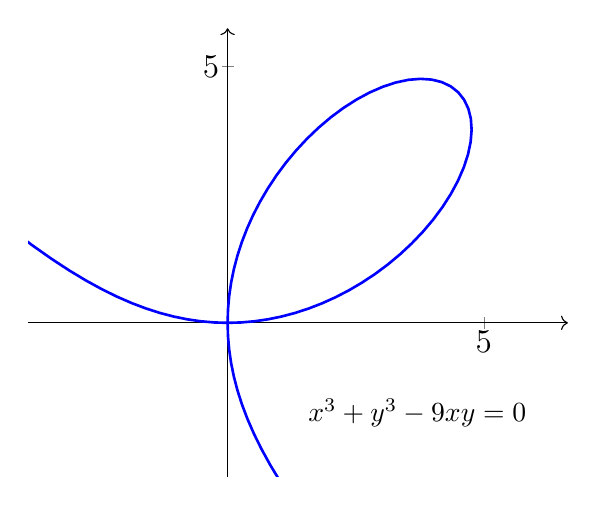
\begin{tikzpicture}
    \begin{axis}[
      axis equal,
      axis lines=center,
      axis line style={->},
      xmin=-3, xmax=5.75,
      ymin=-3, ymax=5.75,
      xtick={-5,5},
      ytick={-5,5},
      ticklabel style={font=\large, inner sep=0.75pt,fill=white},
      ]
      \draw[samples=100,domain=125:-40, line width=0.95pt, blue] plot(\x:{9*sin(\x)*cos(\x)/(sin(\x)^3+cos(\x)^3)}) node[black] at (3.7,-1.75) {$x^3+y^3-9xy=0$};
    \end{axis}
  \end{tikzpicture}
\vfill 
\end{center}
\pagebreak

\begin{center}\fbox{\parbox{0.7\linewidth}{

\textbf{Implicit Differentiation:}
  \begin{enumerate}
    \item Differentiate both sides of the equation with respect to $x$, treating $y$ as a differentiable function of $x$.
    \item Collect the terms with $\sfrac{dy}{dx}$ on one side of the equation.
    \item Solve for $\sfrac{dy}{dx}$.
  \end{enumerate}
}}\end{center}

\begin{ex*}
  Find the derivatives of the following by rewriting each function explicitly before taking the derivative, and by using implicit differentiation. Compare the results.
\end{ex*}

\begin{enumerate}[label=, itemsep=\stretch{1}]
  \item $y^2=x$
  \item $\sqrt x+\sqrt y=4$
\end{enumerate}
\vfill 
\pagebreak
\begin{ex*}
  Find the derivatives of the following equations:
\end{ex*}

\begin{tasks}[after-item-skip=\stretch{1}, label=~](2)
  \task $x^2+y^2=25$
  \task $x^3+y^3-9xy=0$
  \task $2y=x^2+\sin y$
  \task $x^2y^2+x\sin y=4$
  \task $y^5+x^2y^3=1+x^4y$
  \task $1+x=\sin\parens{xy^2}$
\end{tasks}
\vfill
\pagebreak

\begin{ex*}
  Find the derivatives of the following equations:
\end{ex*}
\begin{tasks}[after-item-skip=\stretch{1}, label=~](2)
  \task $x^3-xy+y^3=1$
  \task $xe^y=x-y$
  \task $\dfrac{1}{x}+\dfrac{1}{y}=1$
  \task $x^2-2x^3y^4+y^2=30y$
  \task $\tan(xy)=x+y$
  \task $x^2=\dfrac{x-y}{x+y}$
\end{tasks}
\vfill
\pagebreak

\begin{ex*}
  Find the second derivative implicitly for the following equations:
\end{ex*}
\begin{tasks}[after-item-skip=\stretch{1}, label=~](1)
  \task $y^2-2x=1-2y$
  \task $xy=\cot(xy)$
  \task $x^3+y^3=1$
  \task $x=e^y$
\end{tasks}
\vfill
\pagebreak

\begin{ex*}
  Find the equation of all lines tangent to the curve $x+y^3-y=1$ at $x=1$.
\end{ex*}
\vfill
%% This royal PITA needs to be compiled using 
%% shell-escape since it uses gnuplot
%%%%% pdflatex -shell-escape impFunc.tex %%%%%
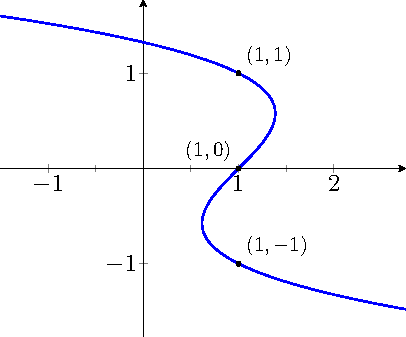
\includegraphics[width=0.4\linewidth]{impFunc1}

\begin{ex*}
  Find the equation of the tangent line and normal line for $\parens{x^2+y^2-2x}^2=2\parens{x^2+y^2}$ at $(x,y)=(2,2)$.  
\end{ex*}
\vfill
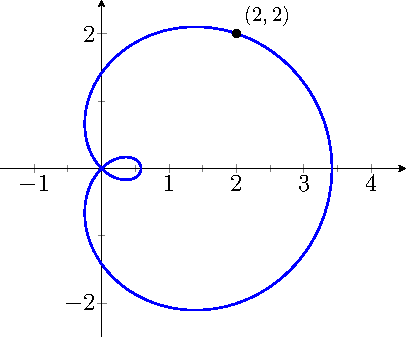
\includegraphics[width=0.4\linewidth]{impFunc2}

\pagebreak

\end{document}

\documentclass[answers]{exam}
\usepackage{texPreamble}
\usepackage{relsize}
\usepackage{tabularx}
\extraheadheight{0.25in}
\extrafootheight{1.0in}
\extrawidth{1in}
% ----------------------------------------------------------------
\firstpagefootrule
\runningfootrule
\begin{document}
%\relscale{1.4}
\section{3.9: Derivatives of Logarithmic and Exponential Functions}
  Recall that $y=\log_a(x)$ and $y=a^x$ are inverse functions:

    \noindent
    \begin{minipage}{0.65\linewidth}
      \fbox{\parbox{0.9875\linewidth}{\centering
        \textbf{Inverse Properites of $a^x$ and $\log_a(x)$}
        
        \begin{enumerate}
          \item $a^{\log_a(x)}=x$, for $x>0$, and $\log_a(a^x)=x$, for all $x$.
          \item $y=\log_a(x)$ if and only if $x=a^y$.
          \item For real numbers $x$ and $b>0$, $b^x=a^{\log_a(b^x)}=a^{x\log_a(b)}$.
        \end{enumerate}
      }}
    \end{minipage}%
    \begin{minipage}{0.35\linewidth}
      \begin{flushright}
        \begin{tikzpicture}[scale=0.8]
          \begin{axis}[
            axis lines=center,
            axis line style={->},
            axis equal,
            xmin=-4.25, xmax=4.25,
            ymin=-4.25, ymax=4.25,
            xmajorticks=false,
            ymajorticks=false,
            ticklabel style={font=\tiny,inner sep=0.75pt,fill=white},
            xlabel=$x$, xlabel style={at={(ticklabel* cs:1)},anchor=north west},
            ylabel=$y$, ylabel style={at={(ticklabel* cs:1)},anchor=south west},
            every axis plot/.append style={line width=1.25pt}
            ]
            \addplot[<->] expression[domain=-5.125:1.45, ClemsonPurple, samples=100] {e^x} node[black, right, pos=0.95, fill=white, xshift=3pt] {$a^x$};
            \addplot[<->] expression[domain=0.0142:5.1, ClemsonOrange,  samples=100] {ln(x)} node[black, above, pos=0.875, fill=white, yshift=5pt] {$\log_a(x)$};
            \addplot[dashed] expression[domain=-5.5:5.5, black!50] {x};
            \addplot[soldot, black, mark size=2pt] coordinates{(0,1)(1,0)};
            \node[anchor = north west] at (1,0) {$(1,0)$};
            \node[anchor = south east] at (0,1) {$(0,1)$};
          \end{axis}
        \end{tikzpicture}
      \end{flushright}
    \end{minipage}%

  \vfill
  \noindent
    \fbox{\parbox{0.9875\linewidth}{
      \textbf{Theorem 3.15: Derivative of $\ln(x)$.}
        $$\ddx\parens{\ln(x)}=\frac{1}{x}, \text{ for } x>0\qquad \ddx\parens{\ln\abs{x}}=\frac{1}{x}, \text{ for } x\neq 0$$
      
      If $u$ is differentiable at $x$ and $u(x)\neq 0$, then
        $$\ddx\parens{\ln\abs{u(x)}}=\frac{u'(x)}{u(x)}$$
    }}
  \vfill
  \begin{center}
    \begin{tikzpicture}
      \begin{groupplot}[
        group style={group size=2 by 1, horizontal sep=50pt},
        axis lines=center,
        axis line style={->},
        xmax=3.75,
        ymin=-4, ymax=4,
        xtick={-5,-3,...,7},
        ytick={-5,-3,...,7},
        ticklabel style={font=\footnotesize,inner sep=0.5pt,fill=white,opacity=1.0, text opacity=1},
        xlabel=$x$, xlabel style={at={(ticklabel* cs:1)},anchor=north west},
        ylabel=$y$, ylabel style={at={(ticklabel* cs:1)},anchor=south west},
        every axis plot/.append style={line width=0.95pt, color=blue}
        ]
        \nextgroupplot[  
          xmin=-0.75, 
          ]
          \addplot[->] expression[domain=exp(-4):3.75, black, samples=301]{ln(x)}
            node[above, pos=0.9] {$y=\ln(x)$};
          \addplot[->] expression[domain=0.25:3.75, red, samples=100]{1/x}
            node[right, pos=0.15] {$y'=\dfrac{1}{x},\ x>0$};
        \nextgroupplot[
          xmin=-3.75, 
          ]
          \addplot[->] expression[domain=exp(-4):3.75, black, samples=301]{ln(x)}
            node[above, pos=0.825, yshift=5pt] {$y=\ln\abs{x}$};
          \addplot[->] expression[domain=0.25:3.75, red, samples=100]{1/x}
            node[left, pos=0.15, xshift=-15pt] {$y'=\dfrac{1}{x}, x\neq0$};
          \addplot[<-] expression[domain=-3.75:-exp(-4), black, samples=301]{ln(-x)};
          \addplot[<-] expression[domain=-3.75:-0.25, red, samples=100]{1/x};
      \end{groupplot}
    \end{tikzpicture}
  \end{center}
  \vfill
  \pagebreak
  
  \begin{ex*}
    Use implicit differentiation to prove $\ds\ddx\ln(x)=\frac{1}{x}$. 
    
    \noindent 
    Then, use the piecewise definition of $\abs{x}$ to prove that $\ds\ddx\ln\abs{x}=\frac{1}{x}$.
  \end{ex*}
  \vfill
  
  \begin{ex*}
    Find the derivatives of the following functions:
  \end{ex*}
  \begin{tasks}[after-item-skip=\stretch{1}, label=~](3)
    \task $y=\ln(x)$
    \task $y=\ln(4x)$
    \task $y=\ln\parens{4x^2+2}$
    \task $f(x)=\sqrt x\ln(x^2)$
    \task $f(x)=\ln\parens{\frac{10}{x}}$
    \task $f(x)=\dfrac{\ln(x)}{1+\ln(x)}$
  \end{tasks}
  \vfill
  
  \pagebreak
  \begin{tasks}[after-item-skip=\stretch{1}, label=~](2)
    \task $f(x)=\sqrt[5]{\ln\parens{3x^4}}$
    \task $f(x)=\ln\sqrt[5]{3x}$
    \task $f(x)=\ln\parens{\ln\parens{\ln(4x)}}$
    \task $f(x)=\ln\abs{x^2-1}$
    \task $y=\ln\parens{\sec^2\theta}$
    \task $y=\parens{\ln\parens{\sin(3x)}}^2$
  \end{tasks}
  \vfill 
  \pagebreak
  
  \noindent
    \fbox{\parbox{0.9875\linewidth}{
      \textbf{Theorem 3.16: Derivative of $b^x$.}
      
      If $b>0$ and $b\neq 1$, then for all $x$.
        $$\ddx\sbrkt{b^x}=b^x\ln(b).$$
    }}
  \begin{ex*}
    Using the properties of exponents and logarithms, prove the above theorem. 
    
    \noindent
    Extend this theorem by stating the derivative of $y=b^{f(x)}$.
  \end{ex*}
  \vfill
  
  \begin{ex*}
    Find the derivatives of the following functions:
  \end{ex*}
  \begin{tasks}[after-item-skip=\stretch{1}, label=~](2)
    \task $y=5^{3x}$
    \task $s(t)=\cos(2^t)$
    \task $g(v)=10^v\parens{\ln(10^v)-1}$
    \task $y=6^{x\ln(x)}$
  \end{tasks}
  \vfill 
  
  \pagebreak
  
  \noindent
    \fbox{\parbox{0.9875\linewidth}{
      \textbf{Theorem 3.18: Derivative of $\log_b(x)$.}
      
      If $b>0$ and $b\neq 1$, then
        \[\ddx\sbrkt{\log_b(x)}=\frac{1}{x\ln b},\text{ for }x>0 \text{ and }\ddx\sbrkt{\log_b\abs{x}}=\frac{1}{x\ln b},\text{ for } x\neq 0.\]
    }}

  \begin{ex*}
    Using the properties of exponents and logarithms, prove the above theorem. 
    
    \noindent
    Extend this theorem by stating the derivative of $y=\log_b\parens{g(x)}$.
  \end{ex*}
  \vfill
  \begin{ex*}
    Find the derivatives of the following functions:
  \end{ex*}
  \begin{tasks}[after-item-skip=\stretch{1}, label=~](2)
    \task $f(x)=\log_4\parens{4x^2+3x}$
    \task $f(x)=\log_5\parens{x e^x}$
    \task $y=2x\log_{10}\sqrt x$
    \task $y=\dfrac{\log_3\parens{\tan\parens{e^2x}}}{\pi\cdot e\inv[4x]}$
  \end{tasks}
  \vfill
  \pagebreak
  
  \begin{center}
    \vfill
    \setlength{\jot}{10pt}
    \noindent
    \fbox{\parbox{0.9875\linewidth}{
      \textbf{Derivative rules for exponential functions:}
      \begin{align*}
        \hspace*{-10pt}
        \ddx \sbrkt{e^x}&=e^x&  \ddx \sbrkt{e^{f(x)}}&=e^{f(x)}\cdot f'(x)\\
        \hspace*{-10pt}
        \ddx \sbrkt{b^x}&=\ln(b)\cdot b^x&  \ddx \sbrkt{b^{g(x)}}&=\ln(b)\cdot b^{g(x)}\cdot g'(x)\hspace*{-10pt}
      \end{align*}
    }}
    \vfill
    
    \fbox{\parbox{0.9875\linewidth}{
      \textbf{Derivative rules for logarithmic functions:}
      \begin{align*}
        \hspace*{-10pt}
        &\ddx\sbrkt{\ln x}=\frac{1}{x}& &\ddx\sbrkt{\ln\parens{f(x)}}=\frac{1}{f(x)}\cdot f'(x)\hspace*{-10pt}\\
        \hspace*{-10pt}
        &\ddx\sbrkt{\log_b(x)}=\frac{1}{\ln(b) x}& &\ddx\sbrkt{\log_b\parens{g(x)}}=\frac{g'(x)}{\ln(b) g(x)}
      \end{align*} 
   }}
   \vfill
   \fbox{\parbox{0.9875\linewidth}{\textbf{Laws of Logarithms}
      
      For $x,y>0$:
      \begin{tasks}[after-item-skip=10pt, label=~](2)
        \task $\log_a(xy)=\log_a(x)+\log_a(y)$
        \task $\log_a\parens{\frac{x}{y}}=\log_a(x)-\log_a(x)$
        \task $\log_a(x^r)=r\log_a(x)$
        \task $\log_a(1)=0$
        \task $\log_a(x)=\dfrac{\log_b(x)}{\log_b(a)}$
        \task $\log_a(a)=1$
      \end{tasks}
    }}
    \vfill
  \end{center}
  \pagebreak
  
  \begin{ex*}
    For the following functions, use the laws of logarithms to rewrite the function before taking the derivative:
  \end{ex*}
  
  \noindent
  \begin{tasks}[after-item-skip=\stretch{1}, label=~](1)
    \task $F(t)=\ln\parens{\dfrac{\parens{2t+1}^3}{\parens{3t+1}^4}}$
    \task $y=\ln\sqrt[3]{\dfrac{1+x}{1-x}}$
    \task $y=\ln\sqrt{\dfrac{\parens{x+1}^5}{\parens{x+2}^{20}}}$
  \end{tasks}
  \vfill 
  
  \pagebreak
  \noindent
  \fbox{\parbox{0.9875\linewidth}{
    \textbf{Logarithmic Differentiation:}
    
    \begin{enumerate}
      \item Take the natural logarithm of both sides of the equation.
      \item Use logarithm laws to simplify.
      \item Use implicit differentiation to take the derivative of both sides.
      \item Solve for $\dydx$.
    \end{enumerate}
  }}
  \begin{ex*}
    Find the derivatives of the following functions:
  \end{ex*}
  \begin{tasks}[after-item-skip=\stretch{1}, label=~](2)
    \task $y=\dfrac{\sin^2(x)\tan^4(x)}{\parens{x^2+1}^2}$
    \task $h(\theta)=\dfrac{\theta \sin(\theta)}{\sqrt{\sec(\theta)}}$
    \task $g(x)=\sqrt[10]{\dfrac{3x+4}{2x-4}}$
    \task $y=\dfrac{e\inv[x]\cos^2(x)}{x^2+x+1}$
  \end{tasks}
  \vfill
  \pagebreak
  
  \noindent
  \textit{Note:} Whenever the function is of the form $f(x)^{g(x)}$, then \textit{Logarithmic Differentiation} is the only option!
  \begin{tasks}[after-item-skip=\stretch{1}, label=~](2)
    \task $y=x^x$
    \task $y=\parens{\ln(x)}^x$
    \task $y=\parens{\tan x}^\frac{1}{x}$
    \task $y=\parens{2x}^{3x}$
  \end{tasks}
  \vfill 
  \pagebreak
  
  \begin{ex*}
    Use the definition of the derivative to evaluate the following limits:
  \end{ex*}
  \begin{tasks}[after-item-skip=\stretch{1}, label=~](2)
    \task $\ds\lim_{x\to e} \dfrac{\ln(x)-1}{x-e}$
    \task $\ds\lim_{h\to 0} \dfrac{\ln(e^8+h)-8}{h}$
    \task $\ds\lim_{x\to 2} \dfrac{5^x-25}{x-2}$
    \task $\ds\lim_{h\to 0} \dfrac{\parens{3+h}^{3+h}-27}{h}$
  \end{tasks}
  \vfill
  \pagebreak
  
  %TODO comment out \relsize!
\end{document}

\documentclass[mathNotesPreamble]{subfiles}
\begin{document}
\tikzset{custNode/.style={color=black,inner sep=0.5pt,fill=none,opacity=1.0, text opacity=1}}
\tikzset{dLine/.style={mark=none, dashed, opacity=1.0, blue!85, line width=0.5pt}}
%\relscale{1.4}
\section{JIT 9.1: Definition of $\arcsin x$, the Inverse Sine Function}
  Recall that a function has an inverse if it is 1-to-1 (e.g. it passes the horizontal line test).
  \begin{center}
    \begin{tikzpicture}
      \begin{groupplot}[
        group style={group size=3 by 1, horizontal sep=1cm},
        width=0.36\linewidth,
        axis lines=center,
        axis line style={->},
        ticklabel style={font=\footnotesize,inner sep=0.5pt,fill=white,opacity=1.0, text opacity=1},
        xlabel=$x$, xlabel style={at={(ticklabel* cs:1)},anchor=north west},
        ylabel=$y$, ylabel style={at={(ticklabel* cs:1)},anchor=south west},
        every axis plot/.append style={line width=0.95pt, color=blue}
        ]
        \nextgroupplot[
          xmin=-4.25, xmax=6.25,
          ymin=-4.25, ymax=6.25,
          xmajorticks=false,
          ymajorticks=false,
          every axis plot/.append style={samples=100},
          ]
          \addplot[dashed] expression[domain=-4.25:6.25, black]{x};
          \addplot[->] expression[domain=-4.25:ln(6.25), ClemsonPurple] {e^x} node[custNode, below right, pos=1] {$a^x$};
          \addplot[->] expression[domain=exp(-4.25):6.25, ClemsonOrange] {ln(x)} node[custNode, above left, pos=1] {$\log_a(x)$};
        \nextgroupplot[
          xmin=-0.5, xmax=3.25,
          ymin=-0.5, ymax=3.25,
          xmajorticks=false,
          ymajorticks=false,
          every axis plot/.append style={samples=500},
          ]
          \addplot[dashed] expression[domain=-0.5:3.25, black]{x};
          \addplot[dashed] expression[domain=-0.5:0, ClemsonPurple]{x^2};
          \addplot[->] expression[domain=0:sqrt(3.25), ClemsonPurple]{x^2} node[custNode, below right, pos=1] {$x^2$};
          \addplot[->] expression[domain=0:3.25, ClemsonOrange]{sqrt(x)} node[custNode, above left, pos=1] {$\sqrt x$};
        \nextgroupplot[
          xmin=-(pi/2+0.5), xmax=(pi/2+0.775),
          ymin=-(pi/2+0.5), ymax=(pi/2+0.65),
          xmajorticks=false,
          ymajorticks=false,
          every axis plot/.append style={samples=100},
          ]
          \addplot[dashed] expression[domain=-(pi/2+0.5):(pi/2+0.775), black]{x};
          \addplot[dashed] expression[domain=-pi/2-0.5:-pi/2, ClemsonPurple]{sin(x*180/pi)};
          \addplot[dashed] expression[domain=pi/2:pi/2+0.775, ClemsonPurple]{sin(x*180/pi)};
          \addplot[-] expression[domain=-pi/2:pi/2, ClemsonPurple]{sin(x*180/pi)} node[custNode, below right, pos=0.85] {$\sin(x)$};
          \addplot[-] expression[domain=-1:1, ClemsonOrange]{asin(x)*pi/180} node[custNode, above, pos=1, xshift=-5pt] {$\arcsin(x)$};
      \end{groupplot}
    \end{tikzpicture}
    
    Notice that $x^2$ and $\sin(x)$ are on restricted domains.
  \end{center}

Without restriction on its domain, $\sin(x)$ is NOT 1-to-1:
\begin{center}
  \begin{tikzpicture}
    \begin{axis}[
      axis lines=center,
      axis line style={->},
      xmin=-7, xmax=7,
      ymin=-1.25, ymax=1.25,
      xtick={-6.28318, -4.7123889, ..., 6.28318},
      xticklabels={$-2\pi$, $-\frac{3\pi}{2}$,$-\pi$, $-\frac{\pi}{2}$, ,
         $\frac{\pi}{2}$,$\pi$, $\frac{3\pi}{2}$, $2\pi$},
      height=1.75in, width=0.9\linewidth,
      ticklabel style={font=\small, inner sep=0.75pt,fill=white},
      xlabel=$x$, xlabel style={at={(ticklabel* cs:1)},anchor=north west},
      ylabel=$y$, ylabel style={at={(ticklabel* cs:1)},anchor=south west},
      every axis plot/.append style={line width=0.95pt, color=blue}
      ]
      \addplot[domain=-6.28:6.28, ClemsonPurple, samples=101] {sin(deg(x))} node[custNode, pos=0.7, above right] {$\sin(x)$};
    \end{axis}
  \end{tikzpicture}
\end{center}

The range of $\sin(x)$ is $[-1,1]$ and all of these values are attained on a restricted domain of $\sbrkt{\nicefrac{-\pi}{2},\nicefrac{\pi}{2}}$:

\begin{center}
  \begin{tikzpicture}
    \begin{groupplot}[
      group style={group size=2 by 1, horizontal sep=4cm},
      axis lines=center,
      axis line style={->},
      xmin=-(pi/2+0.95), xmax=pi/2+0.95,
      ymin=-(pi/2+0.95), ymax=pi/2+0.95,
      width=0.4\linewidth,
      ticklabel style={font=\small, inner sep=0.75pt,fill=white},
      xlabel=$x$, xlabel style={at={(ticklabel* cs:1)},anchor=north west},
      ylabel=$y$, ylabel style={at={(ticklabel* cs:1)},anchor=south west},
      every axis plot/.append style={line width=0.95pt, color=blue, samples=100}      
      ]
      \nextgroupplot[
        xtick={-1.570796327,1.570796327},
        ytick={-1,1},
        xticklabels={$-\frac{\pi}{2}$,$\frac{\pi}{2}$},
        ]
        \addplot[-] expression[domain=-pi/2:pi/2, ClemsonPurple]{sin(x*180/pi)};
        \node[custNode] at (-pi/2,1) {$\sin(x)$};
        \addplot[soldot, black] coordinates{(-pi/2,-1)} node[custNode, below, xshift=5pt, yshift=-4pt] {$\parens{\frac{-\pi}{2},-1}$};
        \addplot[soldot, black] coordinates{(pi/2,1)} node[custNode, above, xshift=5pt, yshift=4pt] {$\parens{\frac{\pi}{2},1}$};
      \nextgroupplot[
        xtick={-1,1},
        ytick={-1.570796327,1.570796327},
        yticklabels={$-\frac{\pi}{2}$,$\frac{\pi}{2}$},
        ]
        \addplot[-] expression[domain=-1:1, ClemsonOrange]{asin(x)*pi/180};
        \node[custNode] at (-pi/2,1) {$\arcsin(x)$};
        \addplot[soldot, black] coordinates{(-1,-pi/2)} node[custNode, below left] {$\parens{-1,\frac{-\pi}{2}}$};
        \addplot[soldot, black] coordinates{(1,pi/2)} node[custNode, above right] {$\parens{1,\frac{\pi}{2}}$};
    \end{groupplot}
  \end{tikzpicture}
\end{center}
  \pagebreak
  
  \begin{defn*}[Inverse Sine and Cosine]
    \def\tmp{5pt}
    $y=\sin\inv(x)$ is the value of $y$ such that $x=\sin(y)$, where $\nicefrac{-\pi}{2}\leq y\leq \nicefrac{\pi}{2}$.\\[\tmp]
    $y=\cos\inv(x)$ is the value of $y$ such that $x=\cos(y)$, where $0\leq y\leq \pi$.\\[\tmp]
    The domain of both $\sin\inv(x)$ and $\cos\inv(x)$ is $\set{x\mid -1\leq x\leq 1}$.
  \end{defn*}

  \textit{Note}: The inverse sine function can be denoted as $\arcsin(x)$ or $\sin\inv(x)$.
  
  This means that $\sin\inv(x)\neq \dfrac{1}{\sin(x)}$. 
  
  Similarly, $\arccos(x)$ and $\cos\inv(x)$ denote the inverse cosine functions.
  \vfill
\begin{center}
  \begin{tikzpicture}
    \begin{groupplot}[
      group style={group size=2 by 1, horizontal sep=2cm},
      axis lines=center,
      axis line style={->},
      width=0.45\linewidth,
      ticklabel style={font=\small, inner sep=0.75pt,fill=white},
      xlabel=$x$, xlabel style={at={(ticklabel* cs:1)},anchor=north west},
      ylabel=$y$, ylabel style={at={(ticklabel* cs:1)},anchor=south west},
      every axis plot/.append style={line width=0.95pt, color=blue, samples=100}      
      ]
      \nextgroupplot[
        xmin=-(pi/2+0.95), xmax=pi/2+0.95,
        ymin=-(pi/2+0.95), ymax=pi/2+0.95,
        xtick={-1.570796327,-1,1,1.570796327},
        ytick={-1.570796327,-1,1,1.570796327},
        xticklabels={$-\frac{\pi}{2}$,-1,1,$\frac{\pi}{2}$},
        yticklabels={$-\frac{\pi}{2}$,-1,1,$\frac{\pi}{2}$},
        ]
        \addplot[-] expression[domain=-pi/2:pi/2, ClemsonPurple]{sin(x*180/pi)} node[custNode, below right, pos=0.95] {$\sin(x)$};
        \addplot[-] expression[domain=-1:1, ClemsonOrange]{asin(x)*pi/180} node[custNode, above, pos=1] {$\sin\inv(x)$};
      \nextgroupplot[
        xmin=-1.5, xmax=pi+0.95,
        ymin=-1.5, ymax=pi+0.95,
        xtick={-1,1,3.141592654},
        ytick={-1,1,3.141592654},
        xticklabels={-1,1,$\pi$},
        yticklabels={-1,1,$\pi$},
        ]
        \addplot[-] expression[domain=0:pi, ClemsonPurple]{cos(x*180/pi)} node[custNode, above right, pos=0.95] {$\cos(x)$};
        \addplot[-] expression[domain=-1:1, ClemsonOrange]{acos(x)*pi/180} node[custNode, above, pos=0.0, xshift=7.5pt, yshift=2.5pt] {$\cos\inv(x)$};
    \end{groupplot}
  \end{tikzpicture}
\end{center}
  \vfill
  \begin{ex*}
    Solve the following:
  \end{ex*}
  \begin{tasks}[after-item-skip=\stretch{1}, label=~](3)
    \task $\sin\inv(0)$
    \task $\arcsin(1)$
    \task $\sin\inv\parens{\dfrac{\sqrt 3}{2}}$
    \task $\cos\inv\parens{-1}$
    \task $\cos\inv\parens{-\dfrac{1}{2}}$
    \task $\arccos\parens{-\dfrac{\sqrt3}{2}}$
  \end{tasks}
  \vfill 
  \pagebreak
\section{JIT 9.2: The Functions $\arctan x$ and $\arcsec x$}
  Similar to $\sin\inv(x)$, we also have inverse functions for the restricted $\tan(x)$ and $\sec(x)$ functions.
  \begin{defn*}[Inverse Tangent and Secant]
    \def\tmp{5pt}
    $y=\tan\inv(x)$ is the value of $y$ such that $x=\tan(y)$, where $\nicefrac{-\pi}{2}< y< \nicefrac{\pi}{2}$.\\[\tmp]
    The domain of $\tan\inv(x)$ is $\set{x\mid -\infty< x< \infty}$.\\[\tmp]
    $y=\sec\inv(x)$ is the value of $y$ such that $x=\sec(y)$, where $0\leq y\leq \pi,\  y\neq\nicefrac{\pi}{2}$.\\[\tmp]
    The domain of $\sec\inv(x)$ is $(-\infty,-1]\cup[1,\infty)$
  \end{defn*}

\begin{center}
  \begin{tikzpicture}
    \def\limOne{4}
    \def\limTwo{4}
    \begin{groupplot}[
      group style={group size=2 by 1, horizontal sep=2cm},
      axis lines=center,
      axis line style={->},
      width=0.425\linewidth,
      ticklabel style={font=\small, inner sep=0.75pt,fill=white},
      xlabel=$x$, xlabel style={at={(ticklabel* cs:1)},anchor=north west},
      ylabel=$y$, ylabel style={at={(ticklabel* cs:1)},anchor=south west},
      every axis plot/.append style={line width=0.95pt, color=blue, samples=100}      
      ]
      \nextgroupplot[
        xmin=-\limOne, xmax=\limOne,
        ymin=-\limOne, ymax=\limOne,
        xtick={-1.570796327,-1,1,1.570796327},
        ytick={-1.570796327,-1,1,1.570796327},
        xticklabels={$-\frac{\pi}{2}$,-1,1,$\frac{\pi}{2}$},
        yticklabels={$-\frac{\pi}{2}$,-1,1,$\frac{\pi}{2}$},
        ]
        \addplot[dLine] coordinates {(-pi/2,-\limOne) (-pi/2,\limOne)};
        \addplot[dLine] coordinates {(pi/2,-\limOne) (pi/2,\limOne)};
        \addplot[dLine] coordinates {(-\limOne,pi/2) (\limOne,pi/2)};
        \addplot[dLine] coordinates {(-\limOne,-pi/2) (\limOne,-pi/2)};
        \addplot[-] expression[domain=-1.32:1.32, ClemsonPurple]{tan(x*180/pi)} node[custNode, right, pos=0.95, xshift=7pt] {$\tan(x)$};
        \addplot[-] expression[domain=-\limOne:\limOne, ClemsonOrange]{atan(x)*pi/180} node[custNode, below right, pos=0.74] {$\tan\inv(x)$};
      \nextgroupplot[
        xmin=-\limTwo, xmax=\limTwo,
        ymin=-\limTwo, ymax=\limTwo,
        xtick={-1.570796327,-1,1,1.570796327,3.14159265},
        ytick={-1.570796327,-1,1,1.570796327,3.14159265},
        xticklabels={$-\frac{\pi}{2}$,-1,1,$\frac{\pi}{2}$,$\pi$},
        yticklabels={$-\frac{\pi}{2}$,-1,1,$\frac{\pi}{2}$,$\pi$},
        ]
        \addplot[dLine] coordinates {(pi/2,-\limTwo) (pi/2,\limTwo)};
        \addplot[dLine] coordinates {(-\limTwo,pi/2) (\limTwo,pi/2)};
        \addplot[-] expression[domain=0:1.5, ClemsonPurple]{1/cos(x*180/pi)} node[custNode, right, pos=0.225, xshift=7.5pt] {$\sec(x)$};
        \addplot[-] expression[domain=1.7:pi, ClemsonPurple]{1/cos(x*180/pi)};
        \addplot[-] expression[domain=-\limTwo:-1, ClemsonOrange]{acos(1/x)*pi/180};
        \addplot[-] expression[domain=1:\limTwo, ClemsonOrange]{acos(1/x)*pi/180} node[custNode, below, pos=0.7] {$\sec\inv(x)$};
    \end{groupplot}
  \end{tikzpicture}
\end{center}
  
  The \textit{Just In Time} book does not include information on $\cos\inv(x), \cot\inv(x)$ and $\csc\inv(x)$. Section 1.4 of \textit{Briggs} provides a very nice reference:
  \vfill 
  \begin{defn*}[Other Inverse Trigonometric Functions]
    \def\tmp{5pt}
    $y=\cot\inv(x)$ is the value of $y$ such that $x=\cot(y)$, where $0< y<\pi$.\\[\tmp]
    The domain of $\cot\inv(x)$ is $\set{x\mid -\infty< x< \infty}$.\\[\tmp]
    $y=\csc\inv(x)$ is the value of $y$ such that $x=\csc(y)$, where $\nicefrac{-\pi}{2}\leq y\leq \nicefrac{\pi}{2},\ y\neq 0$.\\[\tmp]
    The domain of $\csc\inv(x)$ is $(-\infty,-1]\cup[1,\infty)$
  \end{defn*}
  \vfill 
  \pagebreak
  
\vfill
  
\begin{center}
  \def\arraystretch{1.5}\tabcolsep=15pt
  \begin{tabular}{@{}LCC@{}}\toprule
    \textnormal{Function}& \lnret[c]{Restricted\\[-10pt]Domain}& \textnormal{Range}\\\midrule
    \sin(x)& [\nicefrac{-\pi}{2},\nicefrac{\pi}{2}]& [-1,1]\\
    \cos(x)& [0,\pi]& [-1,1]\\
    \tan(x)& \parens{\nicefrac{-\pi}{2},\nicefrac{\pi}{2}}& (-\infty,\infty)\\
    \cot(x)& (0,\pi)& (-\infty,\infty)\\
    \sec(x)& [0,\nicefrac{\pi}{2})\cup (\nicefrac{\pi}{2},\pi]& (-\infty,-1]\cup[1,\infty)\\
    \csc(x)& [\nicefrac{-\pi}{2},0)\cup(0,\nicefrac{\pi}{2}]& (-\infty,-1]\cup[1,\infty)\\\bottomrule
  \end{tabular}
\end{center}  
\vfill

\begin{center}
  \def\arraystretch{1.5}\tabcolsep=15pt
  \begin{tabular}{@{}LCC@{}}\toprule
   \textnormal{Function}& \textnormal{Domain}& \textnormal{Range}\\\midrule
    \sin\inv(x) &  [-1,1] &  [\nicefrac{-\pi}{2},\nicefrac{\pi}{2}] \\
    \cos\inv(x) &  [-1,1] &  [0,\pi] \\
    \tan\inv(x) &  (-\infty,\infty) &  \parens{\nicefrac{-\pi}{2},\nicefrac{\pi}{2}} \\
    \cot\inv(x) &  (-\infty,\infty) &  (0,\pi) \\
    \sec\inv(x) &  (-\infty,-1]\cup[1,\infty) &  [0,\nicefrac{\pi}{2})\cup (\nicefrac{\pi}{2},\pi]\\
    \csc\inv(x) &  (-\infty,-1]\cup[1,\infty) &  [\nicefrac{-\pi}{2},0)\cup(0,\nicefrac{\pi}{2}] \\
\bottomrule
  \end{tabular}
\end{center}
\vfill
\pagebreak
\vfill

\begin{center}
  \def\limOne{4}
  \def\limTwo{4}
  \def\limThree{4}
  \def\limFour{4}
  \begin{tikzpicture}
    \begin{groupplot}[
      group style={group size=2 by 3, horizontal sep=2cm},
      width=0.44\linewidth,
      axis lines=center,
      axis line style={->},
      ticklabel style={font=\footnotesize,inner sep=0.5pt,fill=white,opacity=1.0, text opacity=1},
      xlabel=$x$, xlabel style={at={(ticklabel* cs:1)},anchor=north west},
      ylabel=$y$, ylabel style={at={(ticklabel* cs:1)},anchor=south west},
      every axis plot/.append style={line width=0.95pt, color=blue, samples=100}
      ]
%%%%%%%%%%%%%%%%%%%%%%%%%%%%%%%%%%%%%%%%%%%%%%%%%%%%%%%%%%%%%%%%%%%%%%%%%%%%%%%
      \nextgroupplot[
        xmin=-(pi/2+0.95), xmax=pi/2+0.95,
        ymin=-(pi/2+0.95), ymax=pi/2+0.95,
        xtick={-1.570796327,-1,1,1.570796327},
        ytick={-1.570796327,-1,1,1.570796327},
        xticklabels={$-\frac{\pi}{2}$,-1,1,$\frac{\pi}{2}$},
        yticklabels={$-\frac{\pi}{2}$,-1,1,$\frac{\pi}{2}$},
        ]
        \addplot[dLine] coordinates {(-1,-\limOne) (-1,\limOne)};
        \addplot[dLine] coordinates {(1,-\limOne) (1,\limOne)};
        \addplot[dLine] coordinates {(-\limOne,1) (\limOne,1)};
        \addplot[dLine] coordinates {(-\limOne,-1) (\limOne,-1)};
        \addplot[-] expression[domain=-pi/2:pi/2, ClemsonPurple]{sin(x*180/pi)} node[custNode, below right, pos=0.95] {$\sin(x)$};
        \addplot[-] expression[domain=-1:1, ClemsonOrange]{asin(x)*pi/180} node[custNode, above, pos=1] {$\sin\inv(x)$};
%%%%%%%%%%%%%%%%%%%%%%%%%%%%%%%%%%%%%%%%%%%%%%%%%%%%%%%%%%%%%%%%%%%%%%%%%%%%%%%
      \nextgroupplot[
        xmin=-1.5, xmax=pi+0.95,
        ymin=-1.5, ymax=pi+0.95,
        xtick={-1,1,3.141592654},
        ytick={-1,1,3.141592654},
        xticklabels={-1,1,$\pi$},
        yticklabels={-1,1,$\pi$},
        ]
        \addplot[dLine] coordinates {(-1,-\limTwo) (-1,\limTwo)};
        \addplot[dLine] coordinates {(1,-\limTwo) (1,\limTwo)};
        \addplot[dLine] coordinates {(-\limTwo,1) (\limTwo,1)};
        \addplot[dLine] coordinates {(-\limTwo,-1) (\limTwo,-1)};
        \addplot[-] expression[domain=0:pi, ClemsonPurple]{cos(x*180/pi)} node[custNode, above right, pos=0.95] {$\cos(x)$};
        \addplot[-] expression[domain=-1:1, ClemsonOrange]{acos(x)*pi/180} node[custNode, above, pos=0.0, xshift=7.65pt, yshift=2.5pt] {$\cos\inv(x)$};
%%%%%%%%%%%%%%%%%%%%%%%%%%%%%%%%%%%%%%%%%%%%%%%%%%%%%%%%%%%%%%%%%%%%%%%%%%%%%%%
      \nextgroupplot[
        xmin=-\limOne, xmax=\limOne,
        ymin=-\limOne, ymax=\limOne,
        xtick={-1.570796327,-1,1,1.570796327},
        ytick={-1.570796327,-1,1,1.570796327},
        xticklabels={$-\frac{\pi}{2}$,-1,1,$\frac{\pi}{2}$},
        yticklabels={$-\frac{\pi}{2}$,-1,1,$\frac{\pi}{2}$},
        ]
        \addplot[dLine] coordinates {(-pi/2,-\limTwo) (-pi/2,\limTwo)};
        \addplot[dLine] coordinates {(pi/2,-\limTwo) (pi/2,\limTwo)};
        \addplot[dLine] coordinates {(-\limTwo,pi/2) (\limTwo,pi/2)};
        \addplot[dLine] coordinates {(-\limTwo,-pi/2) (\limTwo,-pi/2)};
        \addplot[-] expression[domain=-1.32:1.32, ClemsonPurple]{tan(x*180/pi)} node[custNode, right, pos=0.95, xshift=7pt] {$\tan(x)$};
        \addplot[-] expression[domain=-\limOne:\limOne, ClemsonOrange]{atan(x)*pi/180} node[custNode, below right, pos=0.75] {$\tan\inv(x)$};
%%%%%%%%%%%%%%%%%%%%%%%%%%%%%%%%%%%%%%%%%%%%%%%%%%%%%%%%%%%%%%%%%%%%%%%%%%%%%%%
      \nextgroupplot[
        xmin=-\limThree, xmax=\limThree,
        ymin=-\limThree, ymax=\limThree,
        xtick={-1,1,3.14159265},
        ytick={-1,1,3.14159265},
        xticklabels={-1,1,$\pi$},
        yticklabels={-1,1,$\pi$},
        ]
        \addplot[dLine] coordinates {(0,-\limTwo) (0,\limTwo)};
        \addplot[dLine] coordinates {(pi,-\limTwo) (pi,\limTwo)};
        \addplot[dLine] coordinates {(-\limTwo,0) (\limTwo,0)};
        \addplot[dLine] coordinates {(-\limTwo,pi) (\limTwo,pi)};
        \addplot[-] expression[domain=0.25:3, ClemsonPurple]{cot(x*180/pi)} node[custNode, right, pos=0.1, xshift=5pt] {$\cot(x)$};
        \addplot[-] expression[domain=-\limThree:-0.0001, ClemsonOrange]{atan(1/x)*pi/180+pi};
        \addplot[-] expression[domain=0.0001:\limThree, ClemsonOrange]{atan(1/x)*pi/180} node[custNode, above, pos=0.73] {$\cot\inv(x)$};
%%%%%%%%%%%%%%%%%%%%%%%%%%%%%%%%%%%%%%%%%%%%%%%%%%%%%%%%%%%%%%%%%%%%%%%%%%%%%%%        
      \nextgroupplot[
        xmin=-\limTwo, xmax=\limTwo,
        ymin=-\limTwo, ymax=\limTwo,
        xtick={-1.570796327,-1,1,1.570796327,3.14159265},
        ytick={-1.570796327,-1,1,1.570796327,3.14159265},
        xticklabels={$-\frac{\pi}{2}$,-1,1,$\frac{\pi}{2}$,$\pi$},
        yticklabels={$-\frac{\pi}{2}$,-1,1,$\frac{\pi}{2}$,$\pi$},
        ]
        \addplot[dLine] coordinates {(pi/2,-\limTwo) (pi/2,\limTwo)};
        \addplot[dLine] coordinates {(-\limTwo,pi/2) (\limTwo,pi/2)};
        \addplot[-] expression[domain=0:1.5, ClemsonPurple]{1/cos(x*180/pi)} node[custNode, right, pos=0.225, xshift=7.5pt] {$\sec(x)$};
        \addplot[-] expression[domain=1.7:pi, ClemsonPurple]{1/cos(x*180/pi)};
        \addplot[-] expression[domain=-\limTwo:-1, ClemsonOrange]{acos(1/x)*pi/180};
        \addplot[-] expression[domain=1:\limTwo, ClemsonOrange]{acos(1/x)*pi/180} node[custNode, below, pos=0.725] {$\sec\inv(x)$};
%%%%%%%%%%%%%%%%%%%%%%%%%%%%%%%%%%%%%%%%%%%%%%%%%%%%%%%%%%%%%%%%%%%%%%%%%%%%%%%
      \nextgroupplot[ 
      xmin=-\limFour, xmax=\limFour,
        ymin=-\limFour, ymax=\limFour,
        xtick={-1.570796327,-1,1,1.570796327,3.14159265},
        ytick={-1.570796327,-1,1,1.570796327,3.14159265},
        xticklabels={$-\frac{\pi}{2}$,-1,1,$\frac{\pi}{2}$,$\pi$},
        yticklabels={$-\frac{\pi}{2}$,-1,1,$\frac{\pi}{2}$,$\pi$},
        ]
        \addplot[dLine] coordinates {(0,-\limTwo) (0,\limTwo)};
        \addplot[dLine] coordinates {(-\limTwo,0) (\limTwo,0)};
        \addplot[-] expression[domain=-1.5:-0.25, ClemsonPurple]{1/sin(x*180/pi)};
        \addplot[-] expression[domain=0.25:1.5, ClemsonPurple]{1/sin(x*180/pi)} node[custNode, right, pos=0.225, xshift=7.5pt] {$\csc(x)$};
        \addplot[-] expression[domain=-\limFour:-1, ClemsonOrange]{asin(1/x)*pi/180};
        \addplot[-] expression[domain=1:\limFour, ClemsonOrange]{asin(1/x)*pi/180} node[custNode, above, pos=0.725] {$\csc\inv(x)$};
%%%%%%%%%%%%%%%%%%%%%%%%%%%%%%%%%%%%%%%%%%%%%%%%%%%%%%%%%%%%%%%%%%%%%%%%%%%%%%%
    \end{groupplot}
  \end{tikzpicture}
\end{center}

\vfill
  \pagebreak
  \begin{ex*}
    Solve the following:
  \end{ex*}
  \begin{tasks}[label=~](3)
    \task $\sin\inv\parens{-\frac{1}{\sqrt{2}}}$
    \task $\sec\inv(2)$
    \task $\cot\inv\parens{-\sqrt{3}}$
  \end{tasks}
  \vspace*{15pt}
  
\section{JIT 9.3: Inverse Trigonometric Identities}
  While $\sin(x)$ and $\sin\inv(x)$ are inverse functions, the inverse relationship only holds when working in the correct domains:
  \begin{tasks}[label=~](2)
    \task $\sin\inv\parens{\sin(\pi)}=\sin\inv(0)=0\neq \pi$
    \task $\sin\parens{\sin\inv(-1)}=\sin\parens{\nicefrac{-\pi}{2}}=-1$
  \end{tasks}
  \vspace*{15pt}
  \begin{ex*}
    Solve the following:
  \end{ex*}
    \begin{tasks}[after-item-skip=\stretch{1}, label=~](2)
      \task $\tan(\tan\inv(5))$
      \task $\tan\inv\parens{\tan\dfrac{3\pi}{4}}$
      \task $\cos\parens{\arcsin\dfrac{1}{2}}$
      \task $\cos\inv\parens{\cos(5\pi)}$
    \end{tasks}
  \vfill
  \pagebreak
  
  \begin{tasks}[after-item-skip=\stretch{1}, label=~](3)
    \task $\sin\inv\parens{\sin\parens{\dfrac{7\pi}{3}}}$
    \task $\tan\parens{\sec\inv(10)}$
    \task $\sin\parens{2\sin\inv\parens{\dfrac{3}{5}}}$
  \end{tasks}
    \vfill
  \begin{ex*}
    Simplify the following using triangles.
  \end{ex*}
  \begin{tasks}[after-item-skip=\stretch{1}, label=~](1)
    \task $\cos\parens{\tan\inv(x)}$
    \task $\sec\parens{\sin\inv(x)}$
    \task $\cos\parens{2\sin\inv(x)}$
    \task $\sin\parens{2\tan\inv(x)}$
  \end{tasks}
  \vfill
  \pagebreak
  
\end{document}

\documentclass[answers]{exam}
\usepackage{texPreamble}
\usepackage{relsize}
\usepackage{tkz-euclide}
\usetkzobj{all}
\usepackage{tabularx}
\extraheadheight{0.25in}
\extrafootheight{1.0in}
\extrawidth{1in}
% ----------------------------------------------------------------
\firstpagefootrule
\runningfootrule
\begin{document}
\tikzset{custNode/.style={color=black,inner sep=0.5pt,fill=none,opacity=1.0, text opacity=1}}
\tikzset{dLine/.style={mark=none, dashed, opacity=1.0, blue!85, line width=0.5pt}}
%%% Need following lines in preamble
%%%%% \usepackage{tkz-euclide} %%%%%
%%%%% \usetkzobj{all}          %%%%%
\newcommand{\blankTriangle}{
      \coordinate (O) at (1.5,6.75);
      \coordinate (A) at (5.5,6.75);
      \coordinate (B) at (5.5,8.75);
      \draw (O)--(A)--(B)--cycle;
      
      \tkzMarkAngle[fill= ClemsonOrange!90,size=1.25cm, opacity=0.8](A,O,B)
      \tkzLabelAngle[pos = 1.0](A,O,B){$y$}
      }
%\relscale{1.4}
\section{3.10: Derivatives of Inverse Trigonometric Functions}
\begin{ex*}
  Recall that $y=\sin\inv(x) \iff \sin(y)=x$. Use this fact and implicit differentiation to derive the derivative of $\sin\inv(x)$.
  \begin{flushright}
    \begin{tikzpicture}[scale=1.0]
      \blankTriangle
      \begin{axis}[
        axis lines=center,
        axis line style={->},
        xmin=-(pi/2+0.95), xmax=pi/2+0.95,
        ymin=-(pi/2+1.5), ymax=pi/2+1.5,
        xtick={-1.570796327,-1,1,1.570796327},
        ytick={-1.570796327,-1,1,1.570796327},
        xticklabels={$-\frac{\pi}{2}$,-1,1,$\frac{\pi}{2}$},
        yticklabels={$-\frac{\pi}{2}$,-1,1,$\frac{\pi}{2}$},
        ticklabel style={font=\small, inner sep=0.75pt,fill=white},
        xlabel=$x$, xlabel style={at={(ticklabel* cs:0.93)},anchor=north west},
        ylabel=$y$, ylabel style={at={(ticklabel* cs:0.9)},anchor=south west},
        every axis plot/.append style={line width=0.95pt, color=blue, samples=100},
        ]
        \addplot[-] expression[domain=-1:1, ClemsonOrange]{asin(x)*pi/180};
        \addplot[-] expression[domain=-0.99:0.99, ClemsonPurple] {1/sqrt(1-x^2)};
        \addplot[dLine] coordinates {(-1,-5) (-1,5)};
        \addplot[dLine] coordinates {(1,-5) (1,5)};
      \end{axis}
    \end{tikzpicture}
  \end{flushright}
  
  \noindent
  Next, extend this definition for the derivative of $\sin\inv(f(x))$.
\end{ex*}
\vspace*{60pt}

\begin{ex*}
  Find the derivative of the following
\end{ex*}
\begin{tasks}[after-item-skip=\stretch{1}, label=~](2)
  \task $\ds f(x)=\sqrt{1-x^2}\,\arcsin(x)$
  \task $\ds y=\sin\inv\parens{\sqrt2 t}$
\end{tasks}
\vspace*{70pt}

\pagebreak
\begin{ex*}
  Recall that $y=\tan\inv(x) \iff \tan(y)=x$. Use this fact and implicit differentiation to derive the derivative of $\tan\inv(x)$.
  \begin{flushright}
    \begin{tikzpicture}[scale=1.0]
      \blankTriangle
      \begin{axis}[
        axis lines=center,
        axis line style={->},
        xmin=-3.5, xmax=3.5,
        ymin=-(pi/2+0.75), ymax=pi/2+0.75,
        xtick={-1.570796327,-1,1,1.570796327},
        ytick={-1.570796327,-1,1,1.570796327},
        xticklabels={$-\frac{\pi}{2}$,-1,1,$\frac{\pi}{2}$},
        yticklabels={$-\frac{\pi}{2}$,-1,1,$\frac{\pi}{2}$},
        ticklabel style={font=\small, inner sep=0.75pt,fill=white},
        xlabel=$x$, xlabel style={at={(ticklabel* cs:0.93)},anchor=north west},
        ylabel=$y$, ylabel style={at={(ticklabel* cs:0.9)},anchor=south west},
        every axis plot/.append style={line width=0.95pt, color=blue, samples=100},
        ]
        \addplot[-] expression[domain=-5:5, ClemsonOrange]{atan(x)*pi/180};
        \addplot[-] expression[domain=-5:5, ClemsonPurple] {1/(x^2+1)};
        \addplot[dLine] coordinates {(-5,pi/2) (5,pi/2)};
        \addplot[dLine] coordinates {(-5,-pi/2) (5,-pi/2)};
      \end{axis}
    \end{tikzpicture}
  \end{flushright}
  \noindent
  Next, extend this definition for the derivative of $\tan\inv(f(x))$.
\end{ex*}
\vspace*{60pt}

\begin{ex*}
  Find the derivative of the following
\end{ex*}
\begin{tasks}[after-item-skip=\stretch{1}, label=~](2)
  \task $\ds y=\sqrt{\tan\inv(x)}$
  \task $\ds y=\tan\inv\parens{\sqrt x}$
\end{tasks}
\vspace*{70pt}  
\pagebreak

\noindent
\fbox{\parbox{0.9875\linewidth}{
\textbf{Derivatives of Inverse Trigonometric Functions}
\begin{center}
  \begin{tabular}{R@{\ =\ }L@{\hspace*{40pt}}R@{\ =\ }L}
    \ds\ddx\sbrkt{\sin\inv(x)}& \dfrac{1}{\sqrt{1-x^2}}& \ds\ddx\sbrkt{\cos\inv(x)}& -\dfrac{1}{\sqrt{1-x^2}}\\[30pt]
    \ds\ddx\sbrkt{\tan\inv(x)}& \dfrac{1}{1+x^2}& \ds\ddx\sbrkt{\cot\inv(x)}& -\dfrac{1}{1+x^2}\\[30pt]
    \ds\ddx\sbrkt{\sec\inv(x)}& \dfrac{1}{\abs{x}\sqrt{x^2-1}}& \ds\ddx\sbrkt{\csc\inv(x)}&-\dfrac{1}{\abs{x}\sqrt{x^2-1}}
  \end{tabular}
\end{center}}}
\vspace*{\stretch{1}}

\noindent
\textbf{Derivative of $y=\sec\inv(x)$}

\begin{center}
  \begin{minipage}{0.3\linewidth}
    \begin{align*}
      y&=\sec\inv(x)\\[7.5pt]
      \sec(y)&=x\\[7.5pt]
      \sec(y)\tan(y)\dydx&=1\\[7.5pt]
      \dydx&=\frac{1}{\sec(y)\tan(y)}
    \end{align*}
  \end{minipage}%
  \hspace*{0.15\linewidth}
  \begin{minipage}{0.3\linewidth}
    \begin{tikzpicture}
      \blankTriangle
      \draw ($(O)!0.5!(B)$) node[above] {$x$};
      \draw ($(A)!0.5!(B)$) node[right] {$\sqrt{x^2-1}$};
      \draw ($(O)!0.5!(A)$) node[below] {$1$};
    \end{tikzpicture}
    
    \vspace*{-15pt}
    \begin{align*}
      \sin^2(x)+\cos^2(x)=1\\[7.5pt]
      \tan^2(x)+1=\sec^2(x)\\[7.5pt]
      1+\cot^2(x)=\csc^2(x)
    \end{align*}
  \end{minipage}%
\end{center}
\vspace*{\stretch{1}}
%Now we rewrite $\sec(y)\tan(y)$ in terms of $x$. 
Note that the restricted domain of $\sec(y)$ is $[0,\nicefrac{\pi}{2})\cup(\nicefrac{\pi}{2},\pi]$, and the restricted domain of $\tan(y)$ is $\parens{-\frac{\pi}{2},\frac{\pi}{2}}$. If we look at these quadrants of the unit circle, we see that the product $\sec(y)\tan(y)$ is always positive, so the resulting derivative must always be positive:
\vspace*{\stretch{1}}
  \[\ddx\sbrkt{\sec\inv(x)}=\frac{1}{\abs{x}\sqrt{x^2-1}}\]
\pagebreak

\begin{ex*}
  Find the derivatives of the following functions:
\end{ex*}
\begin{tasks}[after-item-skip=\stretch{1}, label=~](2)
  \task $h(t)=e^{\sec\inv(t)}$
  \task $y=\arccos\parens{e^{2x}}$
  \task $y=\sin\inv(2x+1)$
  \task $y=\sec\inv(5r)$
  \task $f(x)=\csc\inv\parens{\tan(e^x)}$
  \task $f(x)=\tan\inv(10x)$
\end{tasks}
\vspace*{\stretch{1}}
\pagebreak

\begin{tasks}[after-item-skip=\stretch{1}, label=~](2)
  \task $y=x\sin\inv(x)+\sqrt{1-x^2}$
  \task $h(t)=\cot\inv(t)+\cot\inv\parens{\frac{1}{t}}$
  \task $f(x)=2x\tan\inv(x)-\ln\parens{1+x^2}$
  \task $f(t)=\ln\parens{\tan\inv(t)}$
\end{tasks}
\vspace*{\stretch{1}}
\begin{ex*}
  Find the equation of the tangent line to $f(x)=\cos\inv(x^2)$ at $\parens{\frac{1}{\sqrt2},\frac{\pi}{3}}$.
\end{ex*}
\vspace*{\stretch{1}}
\begin{ex*}
  Find the equation of the tangent line to $f(x)=\sec\inv(e^x)$ at $\parens{\ln(2),\frac{\pi}{3}}$.
\end{ex*}
\vspace*{\stretch{1}}
\pagebreak

\end{document}

\documentclass[answers]{exam}
\usepackage{texPreamble}
\usepackage{relsize}
\usepackage{tabularx}
\extraheadheight{0.25in}
\extrafootheight{1.0in}
\extrawidth{1in}
% ----------------------------------------------------------------
\firstpagefootrule
\runningfootrule
\begin{document}
%\relscale{1.4}
\section{3.11: Related Rates}
  \fbox{\parbox{0.9875\linewidth}{Related rates are problems that use a mathematical relationship between two or more objects under specific constraints. From this, we can differentiate this relationship and examine how each variable changes with respect to time.}}

\begin{ex*}
  An oil rig springs a leak in calm seas and the oil spreads in a circular patch around the rig. If the radius of the oil patch increases at a rate of $30m/hr$, how fast is the area of the patch increasing when the patch has a radius of $100 m$?
\end{ex*}
\vspace*{\stretch{0.4}}
\noindent
\textbf{Solution:}

\begin{center}
  \begin{minipage}{0.95\linewidth}
    We are given the radius $r=100\,m$ which is increasing at a rate of $\frac{dr}{dt}=30\,m/hr$. First, we note the formula for the area of a circle:
  \end{minipage}
  
  \vspace*{-5pt}
  \noindent
  \begin{minipage}[t]{0.65\linewidth}~
    \begin{align*}
      A&=\pi r^2\\
      \intertext{Now, we differentiate \textit{with respect to time} $t$:}
      \frac{dA}{dt}&=2\pi r\frac{dr}{dt}
    \end{align*}
  \end{minipage}%
  \begin{minipage}[t]{0.3\linewidth}~
    \begin{flushright}
      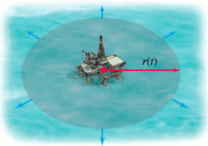
\includegraphics[width=\linewidth]{images/briggs_03_11/oilSpill.png}
    \end{flushright}
  \end{minipage}%
  
  \noindent
  \begin{minipage}{0.95\linewidth}
    Note that we want to solve for $\dfrac{dA}{dt}$ --- the rate of change of the area of the oil patch:
      $$\frac{dA}{dt}=2\pi\parens{100\,m}\parens{30\,m/hr}=6000\pi\, m^2/hr$$
  \end{minipage}
\end{center}
\vspace*{\stretch{1}}

\pagebreak
\begin{ex*}
  Two small planes approach an airport, one flying due west at $120\,mi/hr$ and the other flying due north at $150\, mi/hr$. Assuming they fly at the same constant elevation, how fast is the distance between the planes changing when the westbound plane is $180\,mi$ from the airport and the northbound plane is $225\,mi$ from the airport?
\end{ex*}
\vspace*{\stretch{0.4}}
\noindent
\textbf{Solution:}

\begin{center}
%  \begin{minipage}{0.95\linewidth}
%    Using the diagram below, we label the triangle formed between the planes and the airport such that the plane flying west is a distance of $x$ miles away from the airport, the plane flying north is $y$ miles away from the airport and the distance between the planes is $z$ miles.
%  \end{minipage}
  
  \noindent
  \begin{minipage}{0.6175\linewidth}~
  
    From the problem statement, we know that 
      \begin{align*}
        x&=180\,mi& y&=225\,mi\\
        \frac{dx}{dt}&=-120\,mi/hr& \frac{dy}{dt}&=-150\,mi/hr
      \end{align*}
      Now we use the Pythagorean theorem to relate the three sides:
      $$x^2+y^2=z^2$$
    Next, we differentiate and get the resulting relationship between the related rates:
      $$2x\,\frac{dx}{dt}+2y\,\frac{dy}{dt}=2z\,\frac{dz}{dt}$$
    Before we solve for $\frac{dz}{dt}$, we must find $z$:
  \end{minipage}%
  \begin{minipage}{0.33250\linewidth}~
    \begin{flushright}
      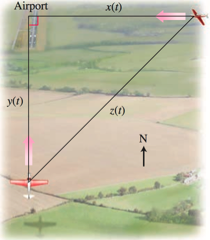
\includegraphics[width=0.95\linewidth]{images/briggs_03_11/airplane.png}
    \end{flushright}
  \end{minipage}
  
  \vspace*{5pt}
  \noindent
  \begin{minipage}{0.95\linewidth}
      $$z=\sqrt{180^2+225^2}=45\sqrt{4^2+5^2}=45\sqrt{41}\approx288\,mi$$
    This gives us
    \begin{align*}
      \frac{dz}{dt}
        =\frac{x\,\frac{dx}{dt}+y\,\frac{dy}{dt}}{z}
        &=\frac{\parens{180\,mi}\parens{-120\,mi/hr}+\parens{225\,mi}\parens{-150\,mi/hr}}{45\sqrt{41}\,mi}\\
        &=\frac{-1230}{\sqrt{41}}\,mi/hr\approx -192\,mi/hr
    \end{align*}
  \end{minipage}
\end{center}
\vspace*{\stretch{1}}

\pagebreak
\begin{center}
  \fbox{\parbox{0.95\linewidth}{
    \textbf{Steps for Related-Rate Problems} 
    \begin{enumerate}
      \item Read the problem carefully, making a sketch to organize the given information. Identify the rates that are given and the rate that is to be determined.
      \item Write one or more equations that express the basic relationships among the variables.
      \item Introduce rates of change by differentiating the appropriate equation(s) with respect to time $t$.
      \item Substitute known values and solve for the desired quantity.
      \item Check that units are consistent and the answer is reasonable. (For example, does it have the correct sign?)
    \end{enumerate}
    }}
\end{center}

\textit{Note:} The \textit{Just-In-Time} book has some examples in chapter 14 that are helpful in setting up the relationships outlined in these types of word problems.
\pagebreak

\begin{ex*}
  A ladder 13 feet long rests against a vertical wall and is sliding down the wall at a constant rate of $3\,ft/s$. How fast is the foot of the ladder moving away from the wall when the foot of the ladder is $5\,ft$ from the base of the wall?
\end{ex*}
\pagebreak

\begin{ex*}
  The volume of a cube decreases at a rate of $0.5\,ft^3/min$. What is the rate of change of the side length when the side lengths are $12\,ft$?
\end{ex*}
\pagebreak

\begin{ex*}
  The length of a rectangle is increasing at a rate of $8\,cm/s$ and its width is increasing at a rate of $3\,cm/s$. When the length is $20\,cm$ and the width is $10\,cm$, how fast is the area of the rectangle increasing?
\end{ex*}
\pagebreak

\begin{ex*}
  A coffee mug has the shape of a right circular cylinder with inner diameter 4 inches and height 5 inches. If the mug is filled with hot chocolate at a constant rate of $2\,in^3/sec$, how fast is the level of the liquid rising?
\end{ex*}
\pagebreak

\begin{ex*}
  A rectangular swimming pool $10\,ft$ wide by $20\,ft$ long and of uniform depth is being filled with water.
\end{ex*}
\begin{enumerate}[label=\alph*), itemsep=\stretch{1}]
  %\item If $t$ is elapsed time, $h$ is the height of the water, and $V$ is the volume of the water, find equations relating $V$ to $h$ and $dV/dt$ to $dh/dt$.
  \item At what rate is the volume of the water increasing if the water level is rising at $\frac{1}{4}\,ft/min$?
  \item At what rate is the water level rising if the pool is filled at a rate of $10\,ft^3/min$?
\end{enumerate}
\vspace*{\stretch{1}}
\pagebreak

\begin{ex*}
  At all times, the length of a rectangle is twice the width $w$ of the rectangle as the area of the rectangle changes with respect to time $t$.
  \begin{enumerate}[label=\alph*), itemsep=\stretch{1}]
    \item Find the equation that relates $A$ to $w$.
    \item Find the equation that relates $dA/dt$ to $dw/dt$.
  \end{enumerate}
\end{ex*}
\vspace*{\stretch{1}}
\pagebreak

\begin{ex*}
  Assume $x,\, y$ and $z$ are functions of $t$ with $z=x+y^3$. Find $dz/dt$ when $dx/dt=-1,\ dy/dt=5$ and $y=2$.
  
\end{ex*}
\vspace*{\stretch{1}}

\begin{ex*}
  Assume $w=x^2y^4$, where $x$ and $y$ are functions of $t$. Find $dw/dt$ when $x=3,\, dx/dt=2,\,dy/dt=4$, and $y=1$.
\end{ex*}
\vspace*{\stretch{1}}
\pagebreak

\begin{ex*}
  The sides of a square decrease in length at a rate of $1\,m/s$.
\end{ex*}
\begin{enumerate}[label=\alph*), itemsep=\stretch{1}]
  \item At what rate is the area of the square changing when the sides are $5\,m$ long?
  \item At what rate are the lengths of the diagonals of the square changing?
\end{enumerate}
\vspace*{\stretch{1}}
\pagebreak

\begin{ex*}
  At noon bicyclist A is 25 miles south of an intersection and bicyclist B is 8 miles west of the same intersection. Bicyclist A is traveling north at 11 miles per hour and bicyclist B is traveling 6 miles per hour west of the intersection. How is the distance between riders changing at 2pm?
\end{ex*}
\pagebreak

\begin{ex*}
  A ladder 13 feet long rests against a vertical wall and is sliding down the wall at a constant rate of $3\,ft/s$. How fast is the angle between the top of the ladder and the wall changing when the angle is $\frac{\pi}{4}$ radians?
\end{ex*}
\pagebreak

\noindent
\begin{minipage}[t]{0.7\linewidth}~
  \begin{ex*}[Piston compression]
    A piston is seated at the top of a cylindrical chamber with radius $5\,cm$ when it starts moving into the chamber at a constant speed of $3\,cm/s$. What is the rate of change of the volume of the cylinder when the piston is $2\,cm$ from the base of the chamber?
  \end{ex*}
\end{minipage}%
\begin{minipage}[t]{0.3\linewidth}~
  \begin{flushright}
    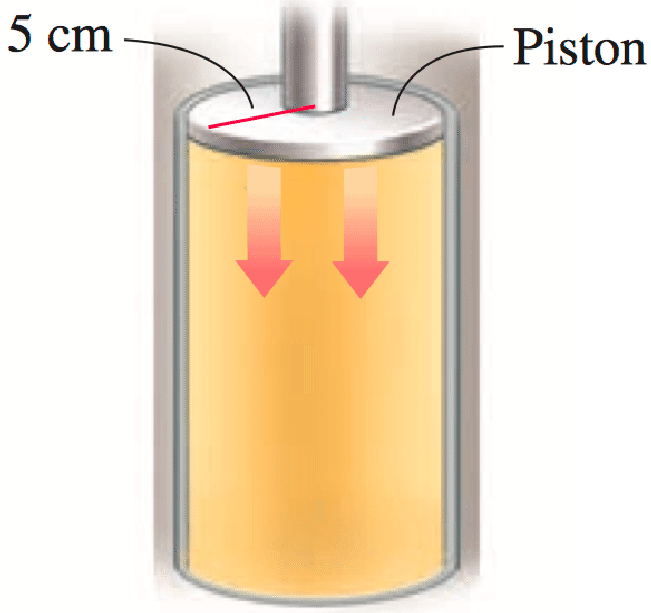
\includegraphics[width=0.9\linewidth]{images/briggs_03_11/piston.png}
  \end{flushright}
\end{minipage}
\pagebreak

\begin{ex*}
  Suppose we have a snowball that is a perfect sphere. If the snowball is melting at a rate of $5\,in^3/min$, how fast is the radius changing when the radius is 10 inches? How fast is the surface area changing?
\end{ex*}
\pagebreak

\noindent
\begin{minipage}{0.7\linewidth}
  \begin{ex*}
    A dinghy is pulled toward a dock by a rope from the bow through a ring on the dock $6\,ft$ above the bow.  The rope is hauled in at a rate of $2\,ft/sec$. At what rate is the angle $\theta$ changing when 10 ft of rope is out?
  \end{ex*}
\end{minipage}%
\begin{minipage}{0.3\linewidth}
  \begin{flushright}
    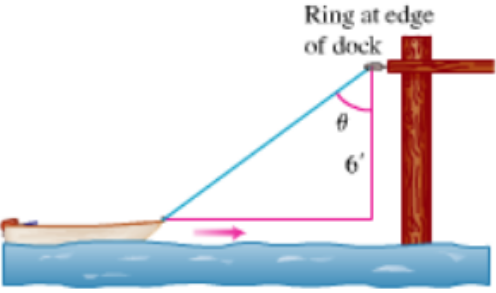
\includegraphics[width=0.9\linewidth]{images/briggs_03_11/dinghy.png}
  \end{flushright}
\end{minipage}
\pagebreak

\begin{ex*}
  At noon, ship A is $150\,km$ west of ship B. Ship A is sailing east at $35\,km/h$ and ship B is sailing north at $25\,km/h$. How fast is the distance between the ships changing at 4pm?
\end{ex*}
\pagebreak

\begin{ex*}
  Once Kate's kite reaches a height of $50\,ft$ (above her hands), it rises no higher but drifts due east in a wind blowing $5\,ft/s$. How fast is the string running through Kate's hands at the moment that she has released $120\,ft$ of string?
\end{ex*}
\pagebreak

\noindent
\begin{minipage}[t]{0.7\linewidth}~
  \begin{ex*}
  Two carts, A and B, are connected by a rope $39\,ft$ long that passes over a pulley $P$. The point $Q$ is on the floor $12\,ft$ directly beneath $P$ and between the carts.  Cart A is being pulled away from $Q$ at  a speed of $2\,ft/s$.  How fast is cart B moving toward $Q$ at the instant when cart A is $5\,ft$ from $Q$?
\end{ex*}
\end{minipage}%
\begin{minipage}[t]{0.3\linewidth}~
  \begin{flushright}
    \vspace*{7.5pt}
    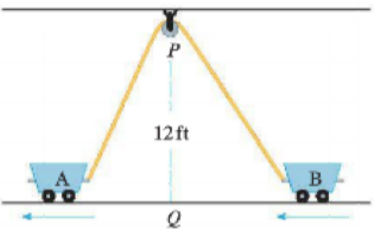
\includegraphics[width=0.9\linewidth]{images/briggs_03_11/cart.png}
  \end{flushright}
\end{minipage}%
\pagebreak

\begin{ex*}
   A camera is set up at the starting line of a drag race 50ft from a dragster at the starting line (camera 1 in the figure). Two seconds after the start of the race, the dragster has traveled 100ft and the camera is turning at 0.75rad/s while filming the dragster.
  \begin{enumerate}[label=\alph*)]
    \item What is the speed of the dragster at this point?
    \item A second camera (camera 2 in the figure) filming the dragster is located on the starting line $100\,ft$ away from the dragster at the start of the race. How fast is this camera turning $2\,s$ after the start of the race?
  \end{enumerate}
\end{ex*}
\vspace*{-20pt}
\begin{flushright}
  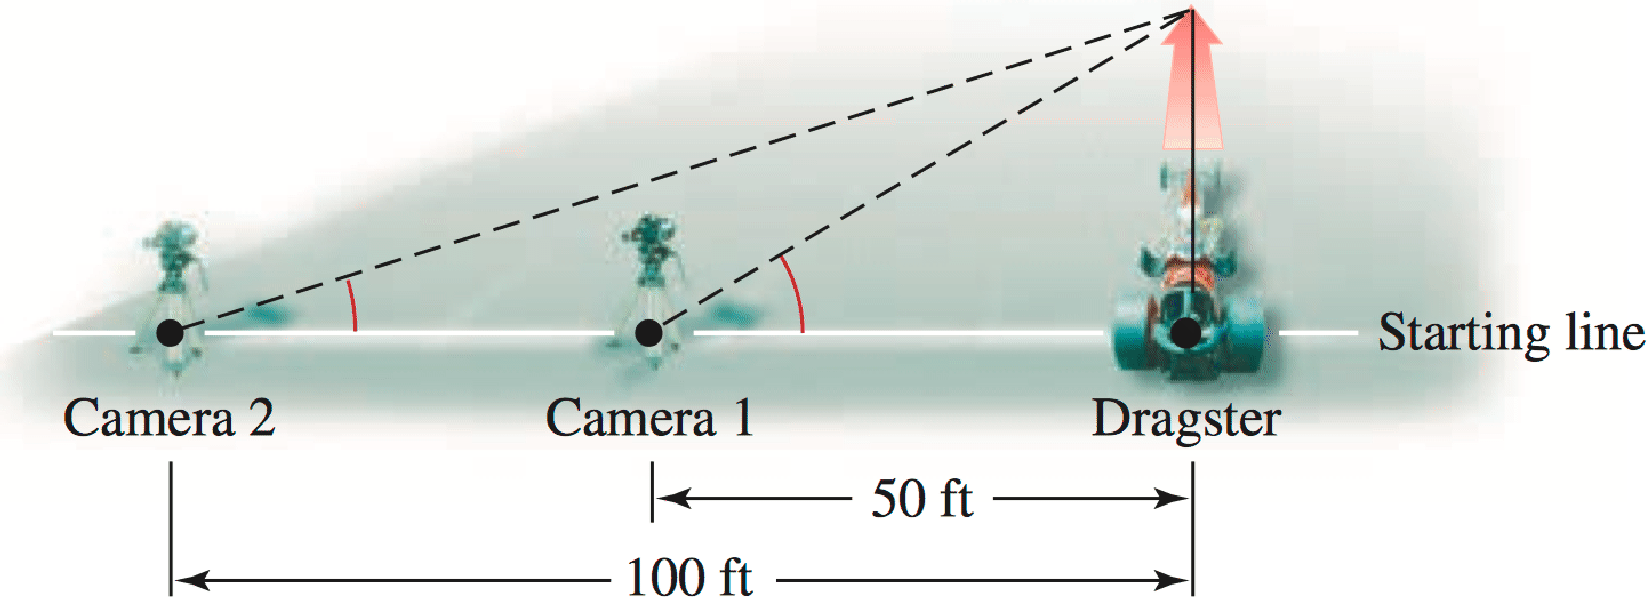
\includegraphics[width=0.5\linewidth]{images/briggs_03_11/dragrace.png}
\end{flushright}
\pagebreak

\begin{ex*}
  A television camera is positioned $4000\,ft$ from the base of a rocket launching pad.  The angle of elevation of the camera has to change at the correct rate in order to keep the rocket in sight. Also the mechanism for focusing the camera has to take into account the increasing distance from the camera to the rising rocket. Assume the rocket rises vertically and its speed is $600\,ft/s$ when it has risen $3000\,ft$. How fast is the distance from the television camera to the rocket changing at that moment? Also, if the television camera is always kept aimed at the rocket, how fast is the camera’s angle of elevation changing at that same moment?
\end{ex*}
\pagebreak
\end{document}
\documentclass[answers]{exam}
\usepackage{texPreamble}
\usepackage{relsize}
\usepackage{tabularx}
\extraheadheight{0.25in}
\extrafootheight{1.0in}
\extrawidth{1in}
% ----------------------------------------------------------------
\firstpagefootrule
\runningfootrule
\begin{document}
%\relscale{1.4}
\section{4.1: Maxima and Minima}
\begin{defn*}[Absolute Maximum and Minimum]
  Let $f$ be defined on a set $D$ containing $c$. 
  \begin{itemize}
    \item 
      If $f(c)\geq f(x)$ for every $x$ in $D$, then $f(c)$ is an \textbf{absolute maximum} value of $f$ on $D$.
    \item 
      If $f(c)\leq f(x)$ for every $x$ in $D$, then $f(c)$ is an \textbf{absolute minimum} value of $f$ on $D$.
    \item 
      An \textbf{absolute extreme value} is either an absolute maximum value or an absolute minimum value.
  \end{itemize}
\end{defn*}
\vspace*{\stretch{1}}
\begin{ex*}
  Determine whether the function has any absolute extreme values
\end{ex*}
\begin{center}
  \begin{tikzpicture}
    \begin{groupplot}[
      group style={group size=3 by 2, horizontal sep=2cm, vertical sep=2cm},
      axis lines=center,
      axis line style={->},
      width=0.3\linewidth,
      ticklabel style={font=\footnotesize,inner sep=0.5pt,fill=white,opacity=1.0, text opacity=1},
      xlabel=$x$, xlabel style={at={(ticklabel* cs:1)},anchor=north west},
      ylabel=$y$, ylabel style={at={(ticklabel* cs:1)},anchor=south},
      every axis plot/.append style={line width=0.95pt, color=blue}
      ]
      \nextgroupplot[
        xmin=-6, xmax=6,
        ymin=-6, ymax=6,
        ylabel=${y=-x^2+4}$, 
        ]
        \addplot[<->] expression[domain=-3:3]{-x^2+4};
      \nextgroupplot[
        xmin=-6, xmax=6,
        ymin=-6, ymax=6,
        ylabel=${y=\frac{x^3}{3}+x^2+1}$,
        ]
        \addplot[<->] expression[domain=-4.125:1.775]{x^3/3+x^2+1};
      \nextgroupplot[
        xmin=-6.75, xmax=6.75,
        ymin=-1.5, ymax=1.5,
        ylabel=${y=\sin(x)}$,
        xtick={-6.28318, -3.141592, ..., 6.28318},
        xticklabels={$-2\pi$,$-\pi$, ,$\pi$, $2\pi$},
        ]
        \addplot[<->] expression[domain=-6.0:6.0, samples=100]{sin(deg(x))};
      \nextgroupplot[
        xmin=-4.5, xmax=4.5,
        ymin=-2, ymax=8.5,
        ylabel=${y=x^2-1}$ on ${[-3,2]}$,
        ]
        \addplot[-] expression[domain=-3:2]{x^2-1};
        \addplot[soldot] coordinates{(-3,8)(2,3)};
      \nextgroupplot[
        xmin=-4.5, xmax=4.5,
        ymin=-2, ymax=8.5,
        ylabel=${y=x^2-1}$ on ${[-3,2)}$,
        ]
        \addplot[-] expression[domain=-3:2]{x^2-1};
        \addplot[holdot] coordinates{(2,3)};
        \addplot[soldot] coordinates{(-3,8)};
      \nextgroupplot[
        xmin=-4.5, xmax=4.5,
        ymin=-2, ymax=8.5,
        ylabel=${y=x^2-1}$ on ${(-3,2)}$,
        ]
        \addplot[-] expression[domain=-3:2]{x^2-1};
        \addplot[holdot] coordinates{(-3,8)(2,3)};
    \end{groupplot}
  \end{tikzpicture}
\end{center}
\vspace*{\stretch{1}}
\pagebreak

\noindent
\fbox{\parbox{0.9875\linewidth}{\textbf{Theorem 4.1: Extreme Value Theorem}

A function that is continuous on a closed interval $\sbrkt{a,b}$ has an absolute maximum value and an absolute minimum value on that interval.
}}

\begin{center}
  \begin{tikzpicture}
    \begin{groupplot}[
      group style={group size=3 by 1, horizontal sep=1.5cm},
      axis lines=center,
      width=0.35\linewidth,
      axis line style={->},
      ticklabel style={font=\footnotesize,inner sep=0.5pt,fill=white,opacity=1.0, text opacity=1},
      xlabel=$x$, xlabel style={at={(ticklabel* cs:1)},anchor=north west},
      ylabel=$y$, ylabel style={at={(ticklabel* cs:1)},anchor=south west},
      every axis plot/.append style={line width=0.95pt, color=blue}
      ]
      \nextgroupplot[
        xmin=-2.5, xmax=3.5,
        ymin=-4.75, ymax=6.25,
        ] 
        \addplot[-] expression[domain=-1.075:3, samples=100]{(x-1)*(x-2)*(x+1)*x*(x-3)+2};
      \nextgroupplot[
        xmin=-2.5, xmax=3.5,
        ymin=-4.5, ymax=6.25,
        ] 
        \addplot[-] expression[domain=-1.075:3, samples=100]{(x-0.5)^2-3};
        \addplot[soldot] coordinates{(-1.075,-0.519375)(3,3.25)};
      \nextgroupplot[
        xmin=-2.5, xmax=3.5,
        ymin=-4.75, ymax=6.25,
        ] 
        \addplot[-] expression[samples=100]{2};
        \addplot[soldot] coordinates{(-2.5,2)(3.5,2)};
    \end{groupplot}
  \end{tikzpicture}
\end{center}
\vspace*{\stretch{1}}
\textit{Note:} It is important that the function is both continuous \textit{and} the interval is closed:
\begin{center}
  \begin{tikzpicture}
    \begin{groupplot}[
      group style={group size=2 by 1, horizontal sep=1.5cm},
      axis lines=center,
      width=0.35\linewidth,
      axis line style={->},
      ticklabel style={font=\footnotesize,inner sep=0.5pt,fill=white,opacity=1.0, text opacity=1},
      xlabel=$x$, xlabel style={at={(ticklabel* cs:1)},anchor=north west},
      ylabel=$y$, ylabel style={at={(ticklabel* cs:1)},anchor=south west},
      every axis plot/.append style={line width=0.95pt, color=blue}
      ]
      \nextgroupplot[
        xmin=0, xmax=3.75,
        ymin=0, ymax=3.75,
        ]
        \addplot[-] expression[domain=1:2]{(x-1)^2+1};
        \addplot[-] expression[domain=2:3, samples=100]{sqrt(3-x)+1.25};
        \addplot[soldot] coordinates{(1,1)(2,2)(3,1.25)};
        \addplot[holdot] coordinates{(2,2.25)};
      \nextgroupplot[
        xmin=-0.5, xmax=2.5,
        ymin=-0.5, ymax=10,
        ymajorticks=false,
        ]
        \addplot[-] expression[domain=0:1.9, samples=100]{1/(2-x)+1/2};
        \draw[densely dashed] (2,-0.5)--(2,10);
        \addplot[holdot] coordinates{(0,1)};
    \end{groupplot}
  \end{tikzpicture}
\end{center}
\vspace*{\stretch{1}}
\pagebreak

\begin{defn*}[Local Maximum and Minimum Values]
  Suppose $c$ is an interior point of some interval $I$ on which $f$ is defined. If $f(c)\geq f(x)$ for all $x$ in $I$, then $f(c)$ is a \textbf{local maximum} value of $f$. If $f(c)\leq f(x)$ for all $x$ in $I$, then $f(c)$ is a \textbf{local minimum value of $f$.}
\end{defn*}

\begin{center}
  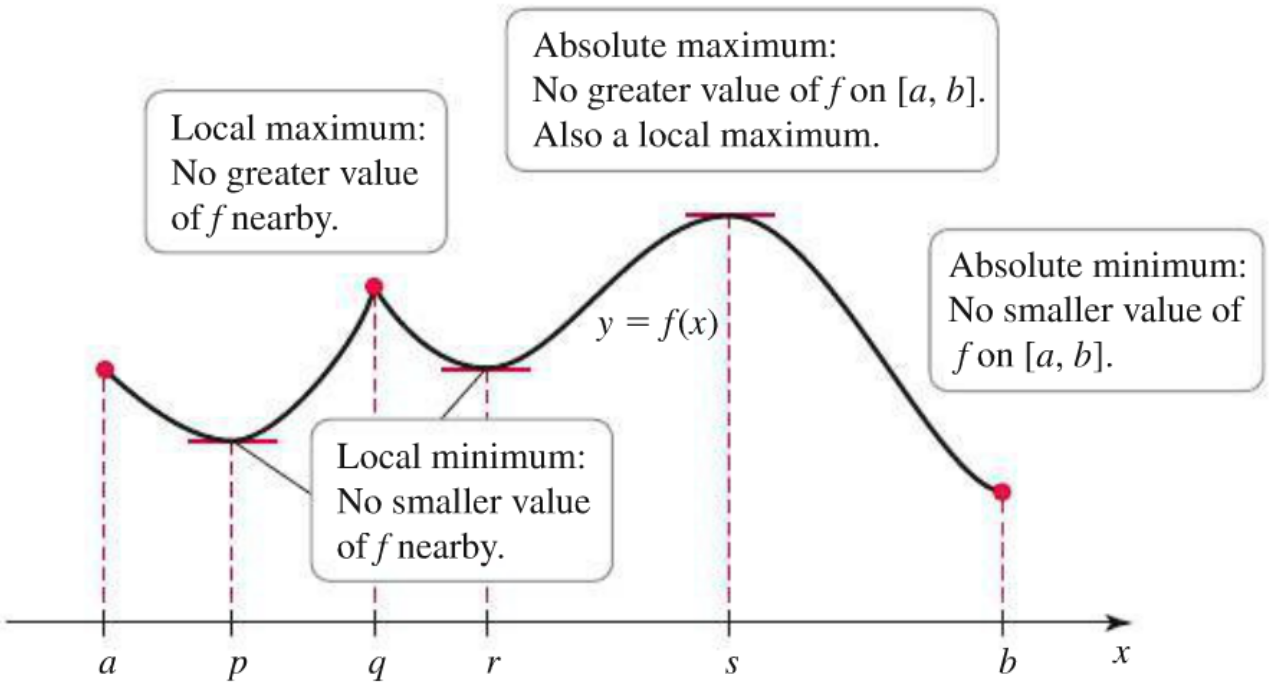
\includegraphics[width=0.55\linewidth]{images/briggs_04_01/fig4_5.png}
\end{center}

\textit{Note:} Local extrema \textbf{CANNOT} occur at endpoints. 

\vspace*{\stretch{1}}
\begin{ex*}
  State the absolute extrema and the local extrema:
\end{ex*}
\begin{center}
  \begin{tikzpicture}
    \begin{groupplot}[
      group style={group size=3 by 2, horizontal sep=1.5cm, vertical sep=1.5cm},
      axis lines=center,
      width=0.325\linewidth,
      axis line style={->},
      ticklabel style={font=\normalsize,inner sep=0.5pt,fill=white,opacity=1.0, text opacity=1},
      xlabel=$x$, xlabel style={at={(ticklabel* cs:1)},anchor=north west},
      ylabel=$y$, ylabel style={at={(ticklabel* cs:1)},anchor=south west},
      every axis plot/.append style={line width=0.95pt, color=blue}
      ]
      \nextgroupplot[
        xmin=1.75, xmax=6,
        ymin=0, ymax=6,
        xtick={2.384,3.506,4.704,5.75},
        xticklabels={$a$, $c_1$, $c_2$, $b$},
        ymajorticks=false,
        ]
        \addplot[-] expression[domain=2.384:5.75, samples=100]{(x-2)*(x-3)*(x-4)*(x-5.125)+2};
        \addplot[soldot] coordinates{(2.384,0.9522)(5.45,6)};
      \nextgroupplot[
        xmin=1.75, xmax=6,
        ymin=0, ymax=3,
        xtick={2.5,4,5.5},
        xticklabels={$a$, $c_1$, $b$},
        ymajorticks=false,
        ]
        \addplot[-] expression[domain=2.5:4,samples=501]{-(4-x)/abs(4-x)*abs(4-x)^(1/3)+2};
        \addplot[-] expression[domain=4:5.5,samples=501]{(4-x)/abs(4-x)*abs(4-x)^(1/3)+2};
        \addplot[holdot] coordinates{(2.5,0.85)(5.5,0.85)};
      \nextgroupplot[
        xmin=-3.5, xmax=2.5,
        ymin=-1.5, ymax=2.5,
        ]
        \addplot[-] expression[domain=-3:0]{-x/3-1};
        \addplot[-] expression[domain=0:1]{3*x-1};
        \addplot[-] expression[domain=1:2]{-2*x+4};
        \addplot[soldot] coordinates{(-3,0)(0,-1)(1,2)(2,0)};
    \end{groupplot}
  \end{tikzpicture}
\end{center}
\vspace*{\stretch{1}}
\pagebreak

\begin{ex*}
  Sketch the graph of a continuous function $f$ on $\sbrkt{0,4}$ satisfying the given properties:
\end{ex*}

\begin{enumerate}
  \item 
    $f'(x)=0$ for $x=1,2$ and $3$; $f$ has an absolute minimum at $x=1$; $f$ has no local extremum at $x=2$; and $f$ has an absolute maximum at $x=3$.

    \begin{tikzpicture}
      \begin{axis}[
        axis lines=center,
        axis line style={->},
        xmin=-0.5, xmax=4.5,
        ymin=-6, ymax=6,
        xtick={-6,-5,...,6},
        height=2.24in,
        width=\linewidth,
        ymajorticks=false,
        ticklabel style={font=\small,inner sep=0.5pt,fill=white,opacity=1.0, text opacity=1},
        ]
      \end{axis}
    \end{tikzpicture}
  \item 
    $f'(1)$ and $f'(3)$ are undefined; $f'(2)=0$; $f$ has a local maximum at $x=1$; $f$ has a local minimum at $x=2$; $f$ has an absolute maximum at $x=3$; and $f$ has an absolute minimum at $x=4$.

    \begin{tikzpicture}
      \begin{axis}[
        axis lines=center,
        axis line style={->},
        xmin=-0.5, xmax=4.5,
        ymin=-6, ymax=6,
        xtick={-6,-5,...,6},
        height=2.24in,
        width=\linewidth,
        ymajorticks=false,
        ticklabel style={font=\small,inner sep=0.5pt,fill=white,opacity=1.0, text opacity=1},
        ]
      \end{axis}
    \end{tikzpicture}
  \item 
    $f'(x)=0$ at $x=1$ and $3$; $f'(2)$ is undefined; $f$ has an absolute maximum at $x=2$; $f$ has neither a local maximum nor a local minimum at $x=1$; and $f$ has an absolute minimum at $x=3$.

    \begin{tikzpicture}
      \begin{axis}[
        axis lines=center,
        axis line style={->},
        xmin=-0.5, xmax=4.5,
        ymin=-6, ymax=6,
        xtick={-6,-5,...,6},
        height=2.24in,
        width=\linewidth,
        ymajorticks=false,
        ticklabel style={font=\small,inner sep=0.5pt,fill=white,opacity=1.0, text opacity=1},
        ]
      \end{axis}
    \end{tikzpicture}
\end{enumerate}
%\vspace*{\stretch{1}}
\pagebreak

\noindent
\fbox{\parbox{0.9875\linewidth}{\textbf{Theorem 4.2: Local Extreme Value Theorem}
  
  If $f$ has a local maximum or minimum value at $c$ and $f'(c)$ exists, then $f'(c)=0$.
}}
\begin{center}
  \textit{Note:} If the derivative is zero, then the function \textbf{MIGHT} have a max/min.  
\end{center}

\begin{ex*}
  Sketch a graph of a function $f(x)$ that has a local maximum value at a point $c$ where $f'(c)$ is defined.
\end{ex*}
\vspace*{\stretch{1}}
\begin{ex*}
  Sketch a graph of a function $f(x)$ that has a local maximum value at a point $c$ where $f'(c)$ is undefined.
\end{ex*}
\vspace*{\stretch{1}}
\begin{ex*}
  Graph 
  \begin{tasks}(2)
    \task $f(x)=x^3$
    \task $f(x)=\abs{x}$
  \end{tasks}
\end{ex*}
\vspace*{\stretch{1}}
\pagebreak
\begin{defn*}[Critical Point]
  An interior point $c$ of the domain of $f$ at which $f'(c)=0$ \textit{or} $f'(c)$ fails to exist is called a \textbf{critical point} of $f$.
\end{defn*}
\begin{ex*}
  Find the critical points of
\end{ex*}
\begin{tasks}[after-item-skip=\stretch{1}, label=~](1)
  \task $f(x)=x^3+3x^2-24x$
  \task $g(x)=\sqrt{4-x^2}$
  \task $h(t)=3t-\sin\inv(t)$
\end{tasks}
\vspace*{\stretch{1}}
\pagebreak
\begin{ex*}
  Find the critical points of
\end{ex*}
\begin{tasks}[after-item-skip=\stretch{1}, label=~](1)
  \task $f(x)=\sin(x)\cos(x)$ on $\sbrkt{0,2\pi}$. 
  \task $f(t)=t^2-2\ln(t^2+1)$
  \task $f(x)=x\sqrt{x-a}$
  \task $f(x)=\sin\inv(x)\cos\inv(x)$
\end{tasks}
\vspace*{\stretch{1}}
\pagebreak
\begin{center}
  \fbox{\parbox{0.8\linewidth}{
    How to find the absolute max/min of $f(x)$ on $\sbrkt{a,b}$:
    \begin{enumerate}
      \item 
        Find $f'(x)$
      \item 
        Find all critical points ($f'(x)=0$ or $f'(x)$ \textbf{DNE})
      \item 
        Evaluate $f(x)$ at the critical points within $\sbrkt{a,b}$ and the end points.
      \item 
        Identify the absolute max and absolute min using the values found. Include value and location (e.g. ordered pair $(x,y)$)
    \end{enumerate}
    }}
\end{center}
\begin{ex*}
  Find the absolute max and min of $f(x)=2x-2x^\frac{2}{3}$ on $\sbrkt{-1,3}$.
\end{ex*}
\vspace*{\stretch{1}}

\begin{ex*}
  Find the absolute max and min of $f(x)=\frac{x}{x^2+1}$ on $\sbrkt{0,2}$.
\end{ex*}
\vspace*{\stretch{1}}

\begin{ex*}
  Find the absolute max and min of $f(x)=3x^4-4x^3-12x^2+1$ on $\sbrkt{-2,3}$.
\end{ex*}
\vspace*{\stretch{1}}
\pagebreak

\begin{ex*}
  Find the absolute max and min of $f(x)=\sin(3x)$ on $\sbrkt{-\frac{\pi}{4},\frac{\pi}{3}}$.
\end{ex*}
\vspace*{\stretch{1}}

\begin{ex*}
  Find the absolute max and min of $f(x)=xe^{1-\frac{x}{2}}$ on $\sbrkt{0,5}$.
\end{ex*}
\vspace*{\stretch{1}}

\begin{ex*}
  Find the absolute max and min of $f(x)=e^x-2x$ on $\sbrkt{0,2}$.
\end{ex*}
\vspace*{\stretch{1}}
\pagebreak

\begin{ex*}
  Find the absolute max and min of $f(x)=x^\frac{1}{3}(x+4)$ on $\sbrkt{-27,27}$.
\end{ex*}
\vspace*{\stretch{1}}

\begin{ex*}
  Find the absolute max and min of $y=\sqrt{x^2-1}$.
\end{ex*}
\vspace*{\stretch{1}}

\begin{ex*}
  Find the absolute/local max and min of $f(x)=x^2\parens{x^2+4x-8}$ on $\sbrkt{-5,2}$.
\end{ex*}
\vspace*{\stretch{1}}
\pagebreak

\begin{ex*}
  \textbf{Minimum-surface-area box} 
  %TODO Future Peter
  % S(x)=2x^2+\frac{4V}{x}
  
  All boxes with a square base of length $x$ and a volume $V$ have a surface area given by $S(x)=x^2+\frac{4V}{x}$. Find $x$ such that the box has volume $50\,ft^3$ with minimal surface area.
\end{ex*}
\vspace*{\stretch{1}}

\begin{ex*}
  \textbf{Trajectory high point}
  
  A stone is launched vertically upward from a cliff $192\,ft$ above the ground at a speed of $64\,ft/s$. Its height above the ground $t$ seconds after the launch is given by $s=-16t^2+64t+192,$ for $0\leq t\leq 6$. When does the stone reach its maximum height?
\end{ex*}
\vspace*{\stretch{1}}
\pagebreak

\begin{ex*}
  \textbf{Maximizing Revenue}
  
  A sales analyst determines that the revenue from sales of fruit smoothies is given by $R(x)=-60x^2+300x$, where $x$ is the price in dollars charged per item, for $0\leq x\leq 5$.
  \begin{enumerate}[label=\alph*)]
    \item 
      Find the critical points of the revenue function.
    \item 
      Determine the absolute maximum value of the revenue function and the price that maximizes the revenue.
  \end{enumerate}
\end{ex*}
\pagebreak

\begin{ex*}
  Find the absolute and local extreme values of the following
  \begin{enumerate}[itemsep=\stretch{1}]
    \item $f(x)=\abs{x-3}+\abs{x+2}$ on $\sbrkt{-4,4}$,
    \item $g(x)=\abs{x-3}-2\abs{x+1}$ on $\sbrkt{-2,3}$.
  \end{enumerate}
\end{ex*}
\vspace*{\stretch{1}}
\pagebreak

\begin{ex*}
  \textbf{Every second counts} (4.01: Q87)
  
  You must get from a point $P$ on the straight shore of a lake to a stranded swimmer who is $50\,m$ from a point $Q$ on the shore that is $50\,m$ from you. Assuming that you can swim at a speed of $2\,m/s$ and run at a speed of $4\,m/s$, the goal of this exercise is to determine the point along the shore, $x$ meters from $Q$, where should you stop running and start swimming to reach the swimmer in the minimum time.

\noindent
\begin{minipage}{0.675\linewidth}
  \begin{enumerate}[label=\alph*)]
    \item 
      Find the function $T$ that gives the travel time as a function of $x$, where $0\leq x\leq 50$.
    \item 
      Find the critical point of $T$ on $(0,50)$.
    \item 
      Evaluate $T$ at the critical point and the endpoints ($x=0$ and $x=50$) to verify that the critical point corresponds to an absolute minimum. What is the minimum travel time?
    \item 
      Graph the function $T$ to check your work.
  \end{enumerate}
\end{minipage}%
\begin{minipage}{0.325\linewidth}
  \begin{flushright}
    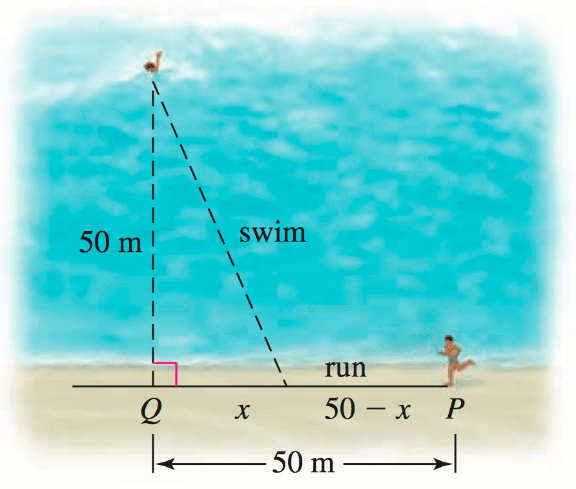
\includegraphics[width=0.95\linewidth]{images/briggs_04_01/swimming_q87.png}
  \end{flushright}
\end{minipage}~
\end{ex*}
\pagebreak

\end{document}

\documentclass[answers]{exam}
\usepackage{texPreamble}
\usepackage{relsize}
\usepackage{tabularx}
\extraheadheight{0.25in}
\extrafootheight{1.0in}
\extrawidth{1in}
% ----------------------------------------------------------------
\firstpagefootrule
\runningfootrule
\begin{document}
%\relscale{1.4}
\section{4.2: Mean Value Theorem}
Before studying the \textit{Mean Value Theorem}, we must first learn \textit{Rolle's Theorem}:\\

\noindent
\fbox{\parbox{0.9875\linewidth}{
\textbf{Theorem 4.3: Rolle's Theorem}

Let $f$ be continuous on a closed interval $[a,b]$ and differentiable on $(a,b)$ with $f(a)=f(b)$. There is at least one point $c$ in $(a,b)$ such that $f'(c)=0$.
}}

\begin{center}
  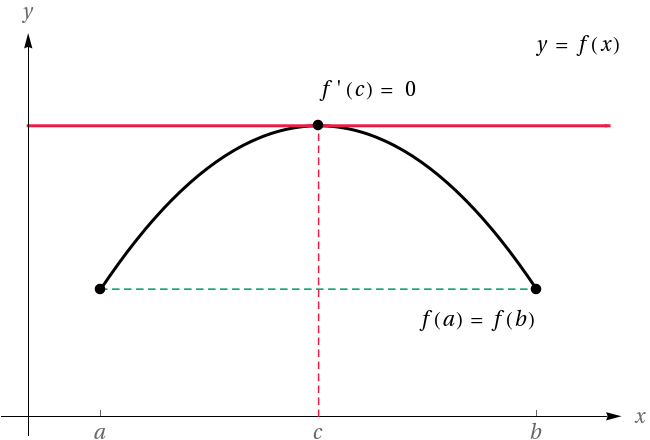
\includegraphics[width=0.3\linewidth]{images/briggs_04_02/RollesThm01.png}
\end{center}

\textit{Note:} Rolle's Theorem requires $f$ be both \textit{continuous} and \textit{differentiable}:
\begin{center}
  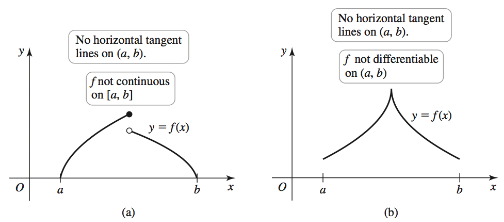
\includegraphics[width=0.6\linewidth]{images/briggs_04_02/RollesThm02.png}
\end{center}

\begin{ex*}
  Determine whether Rolle's Theorem applies for the following. If it applies, find the point(s) $c$ such that $f'(c)=0$.
\end{ex*}
$f(x)=\sin(2x)$ on $\sbrkt{0, \frac{\pi}{2}}$
\pagebreak

\noindent
\fbox{\parbox{0.9875\linewidth}{
\textbf{Theorem 4.4: Mean Value Theorem}

If $f$ is continuous on a closed interval $[a,b]$ and differentiable on $(a,b)$, then there is at least one point $c$ in $(a,b)$ such that 
$\frac{f(b)-f(a)}{b-a}=f'(c)$.
}}

\begin{center}
  \begin{tikzpicture}
    \begin{axis}[declare function={
      f(\x)=(\x)*(\x-1.5)*(\x-2);
      fp(\x)=3*(\x)^2-7*(\x)+3;
      a=0.125; b=0.875; c=0.4657248399474699;},
      axis lines=center,
      axis line style={->},
      width=0.4\linewidth,
      xmin=-0.25, xmax=2.25,
      ymin=-0.5, ymax=1.2,
      ticklabel style={font=\footnotesize,inner sep=0.5pt,fill=white,opacity=1.0, text opacity=1},
      xlabel=$x$, xlabel style={at={(ticklabel* cs:1)},anchor=north west},
      ylabel=$y$, ylabel style={at={(ticklabel* cs:1)},anchor=south west},
      every axis plot/.append style={line width=0.95pt, color=blue, samples=100}
      ]
      \addplot[-] expression[domain=-0.2:2.5]{f(x)};
      \addplot[-, red] expression[domain=-0.2:2.5]{fp(c)*(x-c)+f(c)};                %tangent line
      \addplot[densely dashed, black] expression[domain=-0.2:2.5]{fp(c)*(x-a)+f(a)}; %secant line
      \addplot[soldot, black] coordinates{(a,{f(a)})} node[below right, xshift=-2pt, yshift=4pt] {$A$};
      \addplot[soldot, black] coordinates{(b,{f(b)})} node[right, xshift=5pt, yshift=-2pt] {$B$};
      \addplot[soldot, black] coordinates{(c,{f(c)})} node[above] {$C$};
    \end{axis}
  \end{tikzpicture}
\end{center}

\begin{ex*}
  For $f(x)=x^\frac{2}{3}$ on the interval $\sbrkt{0,1}$, does the Mean Value Theorem apply? If so, find the point(s) $c$ such that $\frac{f(b)-f(a)}{b-a}=f'(c)$
\end{ex*}
\pagebreak

\begin{ex*}
  For each function, associated interval and graph determine if the conditions for the Mean Value Theorem are met and find the value(s) of $c$ such that $\dfrac{f(b)-f(a)}{b-a}=f'(c)$.
\end{ex*}
\begin{enumerate}
  \def\width{0.38\linewidth}
  \item 
    $f(x)=\dfrac{x^2}{4}+1$ on $\sbrkt{-2,4}$
    
    \begin{tikzpicture}
      \begin{axis}[
        grid=both,
        grid style={line width=0.35pt, draw=gray!75},
        axis lines=center,
        axis line style={-},
        width=\width,
        xmin=-3, xmax=5,
        ymin=0, ymax=6,
        xtick={-6,-5,...,6},
        ytick={-6,-5,...,6},
        ticklabel style={font=\footnotesize,inner sep=0.5pt,fill=white,opacity=1.0, text opacity=1},
        every axis plot/.append style={line width=0.95pt, color=blue, samples=100}
        ]
        \addplot[-] expression[domain=-3:5]{x^2/4+1};
        \addplot[-] expression[domain=-3:5, red]{0.5*x+3};
      \end{axis}
    \end{tikzpicture}
  \item 
    $f(x)=2\sqrt{x}$ on $\sbrkt{0,4}$
    
    \begin{tikzpicture}
      \begin{axis}[
        grid=both,
        grid style={line width=0.35pt, draw=gray!75},
        axis lines=center,
        axis line style={-},
        width=\width,
        xmin=0, xmax=4,
        ymin=0, ymax=4,
        xtick={-6,-5,...,6},
        ytick={-6,-5,...,6},
        ticklabel style={font=\footnotesize,inner sep=0.5pt,fill=white,opacity=1.0, text opacity=1},
        every axis plot/.append style={line width=0.95pt, color=blue, samples=501}
        ]
        \addplot[-] expression[domain=0:4]{2*sqrt(x)};
        \addplot[-] expression[domain=0:4, red]{x};
      \end{axis}
    \end{tikzpicture}
  \item 
    $f(x)=\dfrac{x^5}{16}$ on $\sbrkt{-2,2}$
    
    \begin{tikzpicture}
      \begin{axis}[
        grid=both,
        grid style={line width=0.35pt, draw=gray!75},
        axis lines=center,
        axis line style={-},
        width=\width,
        xmin=-3.5, xmax=3.5,
        ymin=-3.5, ymax=3.5,
        xtick={-6,-5,...,6},
        ytick={-6,-5,...,6},
        ticklabel style={font=\footnotesize,inner sep=0.5pt,fill=white,opacity=1.0, text opacity=1},
        every axis plot/.append style={line width=0.95pt, color=blue, samples=100}
        ]
        \addplot[-] expression[domain=-3:3]{x^5/16};
        \addplot[-] expression[domain=-3:3, red]{x};
      \end{axis}
    \end{tikzpicture}
\end{enumerate}
\pagebreak

\begin{ex*}
  Determine whether Rolle's Theorem applies to the following functions and find the point(s) $c$ if applicable.
\end{ex*}
\begin{enumerate}[itemsep=\stretch{1}]
  \item $f(x)=x(x-1)^2$ on $\sbrkt{0,1}$.
  \item $f(x)=x^3-x^2-5x-3$ on $\sbrkt{-1,3}$.
\end{enumerate}
\vspace*{\stretch{1}}

\begin{ex*}
  Determine whether the Mean Value Theorem applies to the following functions and find the point(s) $c$ if applicable.
\end{ex*}
\begin{enumerate}[itemsep=\stretch{1}]
  \item $f(x)=3x^2+2x+5$ on $\sbrkt{-1,1}$.
  \item $f(x)=x\inv[\frac{1}{3}]$ on $\sbrkt{\frac{1}{8},8}$.
\end{enumerate}
\vspace*{\stretch{1}}
\pagebreak
\begin{enumerate}[itemsep=\stretch{1}]
  \setcounter{enumi}{2}
  \item $f(x)=\begin{cases}
      \frac{\sin(x)}{x},& -\pi\leq x<0\\
      0,& x=0
    \end{cases}$.
  \item $f(x)=\abs{x-1}$ on $\sbrkt{-1,4}$.
\end{enumerate}
\vspace*{\stretch{1}}
\begin{ex*}[Mean Value Theorem and graphs]
  
  \noindent
  Locate all points on the graph at which the slope of the tangent line equals the secant line on the interval $\sbrkt{-4,4}$.
\end{ex*}
  
\begin{center}
  \begin{tikzpicture}
    \begin{axis}[
      axis lines=center,
      axis line style={->},
      xmin=-5.5, xmax=5.5,
      ymin=-3.5, ymax=4.5,
      xtick={-6,-4,...,6},
      ytick={-6,-4,...,6},
      minor x tick num=1,
      minor y tick num=1,
      ticklabel style={font=\footnotesize,inner sep=0.5pt,fill=white,opacity=1.0, text opacity=1},
      xlabel=$x$, xlabel style={at={(ticklabel* cs:1)},anchor=north west},
      ylabel=$y$, ylabel style={at={(ticklabel* cs:1)},anchor=south west},
      every axis plot/.append style={line width=0.95pt, color=blue, samples=100}
      ]
      \addplot[-] expression[domain=-4:4]{(x+3.75)*(x+1)*x*(x-3.5)/20};
      \addplot[soldot,red] coordinates{(-4,1.125)(4,3.875)};
      \draw[-] (-4,1.125)--(4,3.875);
    \end{axis}
  \end{tikzpicture}
\end{center}
\pagebreak

\begin{ex*}
  Find the number that satisfies the hypotheses of the Mean Value Theorem for $f(x)=\sqrt x$ on $\sbrkt{0,4}$. Graph the function, the secant line through the endpoints, and the tangent line at $c$, visually verify that the secant and tangent are parallel.
\end{ex*}
\vspace*{\stretch{1}}

\begin{ex*}[Drag racer acceleration]
  
  \noindent
  The fastest drag racers can reach a speed of $330\,mph$ over a quarter-mile strip in $5\,s$ (from a standing start). At some point during the race, the maximum acceleration of the drag racer is at least \underline{\hspace*{50pt}}$\,mph/s$.
\end{ex*}
\vspace*{\stretch{1}}

\begin{ex*}
  A state patrol officer saw a car start from rest at a highway on-ramp. She radioed ahead to another officer 35 miles from the on-ramp. When the car reached the location of the second officer, 30 minutes later, it was clocked going $60\,mph$. The driver of the car was given a ticket for exceeding the $65\,mph$ speed limit. Why can the officer conclude that the driver exceeded the speed limit?
\end{ex*}
\vspace*{\stretch{1}}
\pagebreak

%TODO remove relsize
\end{document}

\documentclass[answers]{exam}
\usepackage{texPreamble}
\usepackage{relsize}
\usepackage{tabularx}
\extraheadheight{0.25in}
\extrafootheight{1.0in}
\extrawidth{1in}
% ----------------------------------------------------------------
\firstpagefootrule
\runningfootrule
\begin{document}
%\relscale{1.4}
\section{4.3: What Derivatives Tell Us}
\begin{defn*}[Increasing and Decreasing Functions]
  Suppose a function $f$ is defined on an interval $I$. We say that $f$ is increasing on $I$ if $f(x_2)>f(x_1)$ whenever $x_1$ and $x_2$ are in $I$ and $x_2>x_1$. We say that $f$ is decreasing on $I$ if $f(x_2)<f(x_1)$ whenever $x_1$ and $x_2$ are in $I$ and $x_2>x_1$.
\end{defn*}
\begin{center}
  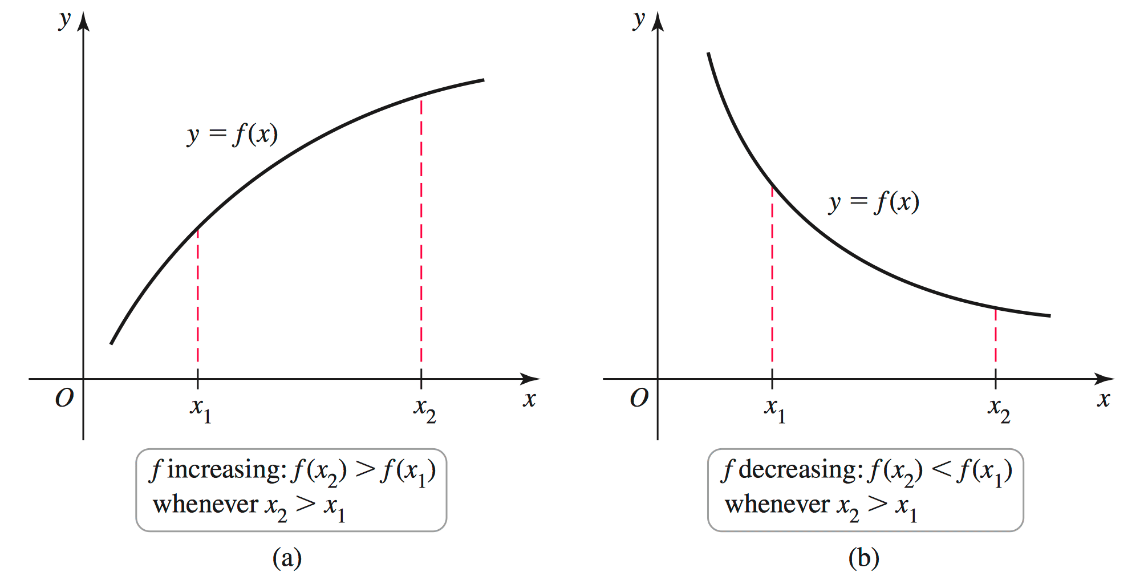
\includegraphics[width=0.65\linewidth]{images/briggs_04_03/fig4_20.png}
\end{center}

\vspace*{\stretch{1}}
\noindent
\fbox{\parbox{0.9875\linewidth}{
  \textbf{Theorem 4.7: Test for Intervals of Increase and Decrease}
  
  Suppose $f$ is continuous on an interval $I$ and differentiable at every interior point of $I$. If $f'(x)>0$ at all interior points of $I$, then $f$ is increasing on $I$. If $f'(x)<0$ at all interior points of $I$, then $f$ is decreasing on $I$.
}}
\begin{center}
  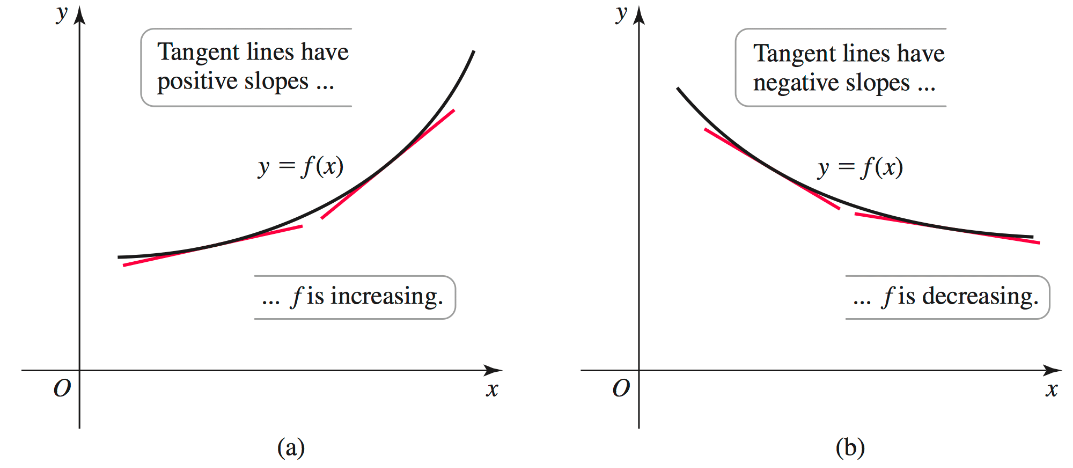
\includegraphics[width=0.65\linewidth]{images/briggs_04_03/fig4_21.png}
\end{center}
\pagebreak
\begin{proof}
  \textbf{(Theorem 4.7: Test for Intervals of Increase and Decrease) p258}

  Let $a$ and $b$ be any two distinct points in the interval $I$ with $b>a$. By the Mean Value Theorem, 
    $$\frac{f(b)-f(a)}{b-a}=f'(c)$$
  for some $c$ between $a$ and $b$. Equivalently,
    $$f(b)-f(a)=f'(c)(b-a).$$
  Notice that $b-a>0$ by assumption. So if $f'(c)>0$, then $f(b)-f(a)>0$. Therefore, for all $a$ and $b$ in $I$ with $b>a$, we have $f(b)>f(a)$, which implies that $f$ is increasing on $I$. Similarly, if $f'(c)<0$, then $f(b)-f(a)<0$ or $f(b)<f(a)$. It follows that $f$ is decreasing on $I$.
\end{proof}
\vspace*{\stretch{1}}

\noindent
\fbox{\parbox{0.9875\linewidth}{
  \textbf{Theorem 4.8: First Derivative Test}
  
  Assume that $f$ is continuous on an interval that contains a critical point $c$ and assume $f$ is differentiable on an interval containing $c$, except perhaps at $c$ itself.

\vspace*{10pt}
  \begin{minipage}{0.85\linewidth}
    \begin{itemize}
      \item If $f'$ changes sign from positive to negative as $x$ increases through $c$, then $f$ has a local maximum at $c$.
      \item If $f'$ changes sign from negative to positive as $x$ increases through $c$, then $f$ has a local minimum at $c$.
      \item If $f'$ does not change sign at $c$ (from positive to negative or vice versa), then $f$ has no local extreme value at $c$.
    \end{itemize}
  \end{minipage}
}}

\begin{center}
  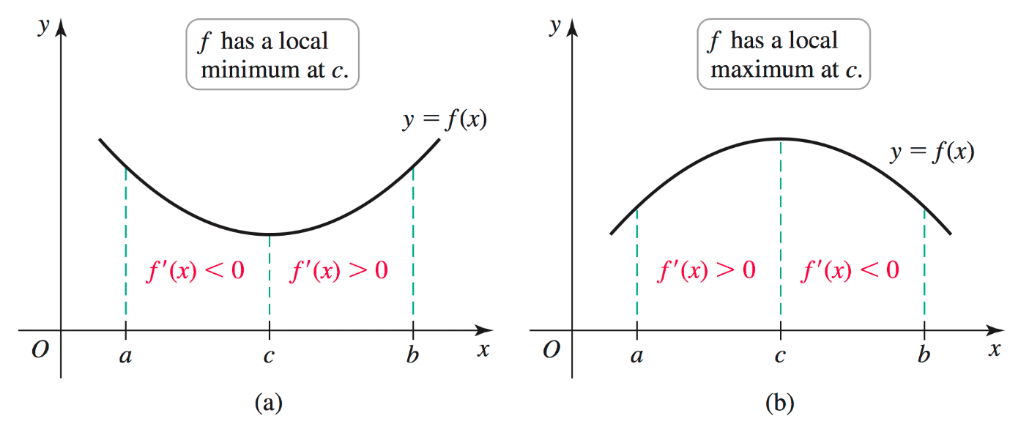
\includegraphics[width=0.65\linewidth]{images/briggs_04_03/fig4_26.png}
\end{center}
\vspace*{-35pt}
\pagebreak

\begin{ex*}
  Consider the function $f(x)=6x-x^3$.
\end{ex*}
  \begin{enumerate}[label=\alph*)]
    \item $f'(x)=$ \\[15pt]
    \item Find the intervals on which the function is increasing and decreasing.
      \setlength\itemsep{\stretch{1}}
    \item Identify the function's local extreme values, if any. (e.g. ``local max of \underline{\hspace*{15pt}} at $x=\underline{\hspace*{15pt}}$'')
    \item Which, if any, of the extreme values are absolute? 
  \end{enumerate}
\vspace*{\stretch{1}}
\pagebreak
\begin{ex*}
  Consider the function $f(t)=12t-t^3$ on $-3\leq t<\infty$.
\end{ex*}
\begin{enumerate}[label=\alph*)]
  \item $f'(t)=$ \\[15pt]
  \item Find the intervals on which the function is increasing and decreasing.
    \setlength\itemsep{\stretch{1}}
  \item Identify the function's local extreme values, if any. (e.g. ``local max of \underline{\hspace*{15pt}} at $x=\underline{\hspace*{15pt}}$'')
  \item Which, if any, of the extreme values are absolute? 
\end{enumerate}
\vspace*{\stretch{1}}
\pagebreak

\begin{ex*}
  Consider the function $f(x)=\cos^2(x)$ on $\sbrkt{-\pi,\pi}$. Find the intervals on which $f$ is increasing and the intervals on which it is decreasing.
\end{ex*}
\vspace*{\stretch{1}}
\pagebreak
\begin{defn*}[Concavity and Inflection Point]
  Let $f$ be differentiable on an open interval $I$. 
  \begin{itemize}
    \item If $f'$ is increasing on $I$, then $f$ is \textit{concave up} on $I$.
   
    \item If $f'$ is decreasing on $I$, then $f$ is \textit{concave down} on $I$.
  
  	\item If $f$ is continuous at $c$ and $f$ changes concavity at $c$, then $f$ has an \textit{inflection point} at $c$.
  \end{itemize}
\end{defn*}

\vspace*{\stretch{1}}
\begin{center}
  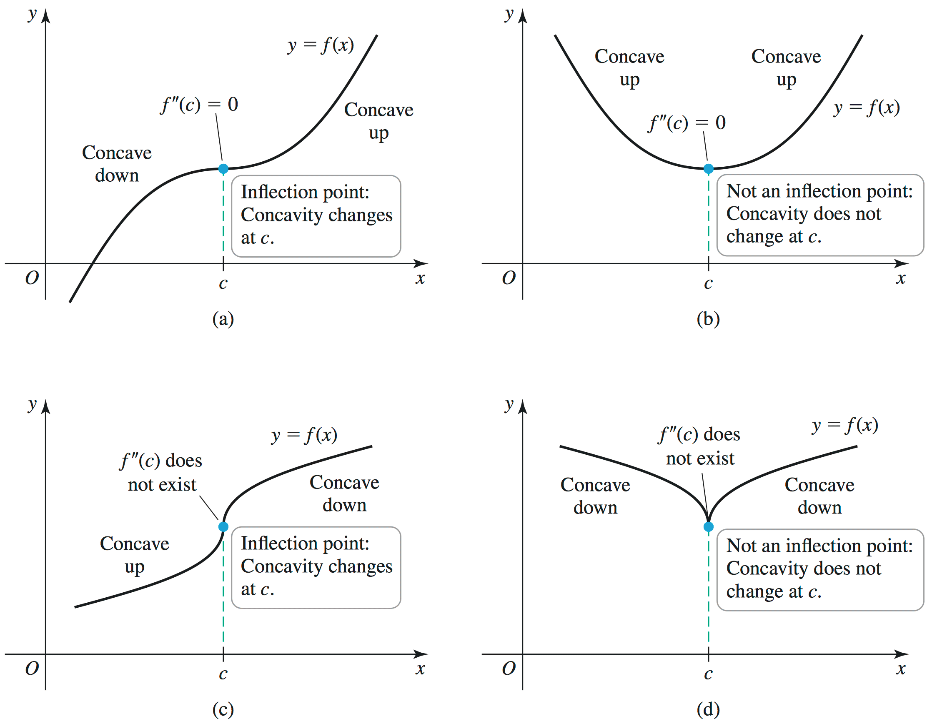
\includegraphics[width=0.925\linewidth]{images/briggs_04_03/fig4_35.png}
\end{center}
\pagebreak

\noindent
\fbox{\parbox{0.9875\linewidth}{
  \textbf{Theorem 4.10: Test for Concavity}
  
  Suppose $f''$ exists on an open interval $I$.
  \begin{itemize}
    \item If $f''>0$ on $I$, then $f$ is concave up on $I$.
    \item If $f''<0$ on $I$, then $f$ is concave down on $I$.
    \item If $c$ is a point of $I$ at which $f''$ changes sign at $c$, then $f$ has an inflection point at $c$.
  \end{itemize}
}}
\begin{ex*}
  Consider $f(x)=5-3x^2+x^3$
\end{ex*}
\begin{enumerate}[itemsep=\stretch{1}, label=\alph*)]
  \item Find the intervals of increasing/decreasing and local max/min.
  \item Find intervals of concavity and inflection points.
  \item Draw a rough sketch of the function.
\end{enumerate}
\vspace*{\stretch{1}}
\pagebreak

\begin{ex*}
  Consider $f(x)=xe\inv[x^2/2]$
\end{ex*}
\begin{enumerate}[itemsep=\stretch{1}, label=\alph*)]
  \item Find the intervals of increasing/decreasing and local max/min.
  \item Find intervals of concavity and inflection points.
  \item Draw a rough sketch of the function.
\end{enumerate}
\vspace*{\stretch{1}}
\pagebreak

\begin{ex*}
  Consider $f(x)=x\,\sqrt[3]{(x-3)^2}$
\end{ex*}
\begin{enumerate}[itemsep=\stretch{1}, label=\alph*)]
  \item Find the intervals of increasing/decreasing and local max/min.
  \item Find intervals of concavity and inflection points.
  \item Draw a rough sketch of the function.
\end{enumerate}
\vspace*{\stretch{1}}
\pagebreak

\begin{ex*}
  Consider $f(x)=x^2-x-\ln(x)$
\end{ex*}
\begin{enumerate}[itemsep=\stretch{1}, label=\alph*)]
  \item Find the intervals of increasing/decreasing and local max/min.
  \item Find intervals of concavity and inflection points.
  \item Draw a rough sketch of the function.
\end{enumerate}
\vspace*{\stretch{1}}
\pagebreak

\begin{ex*}
  Given the first derivative $y'=\parens{x-2}\inv[1/3]$
\end{ex*}
\begin{enumerate}[itemsep=\stretch{1}, label=\alph*)]
  \item Find the intervals of increasing/decreasing and local max/min of $y$.
  \item Find intervals of concavity and inflection points.
  \item Draw a rough sketch of the function.
\end{enumerate}
\vspace*{\stretch{1}}
\pagebreak

As a visual summary, here is figure 4.27 from Briggs:
\begin{center}
  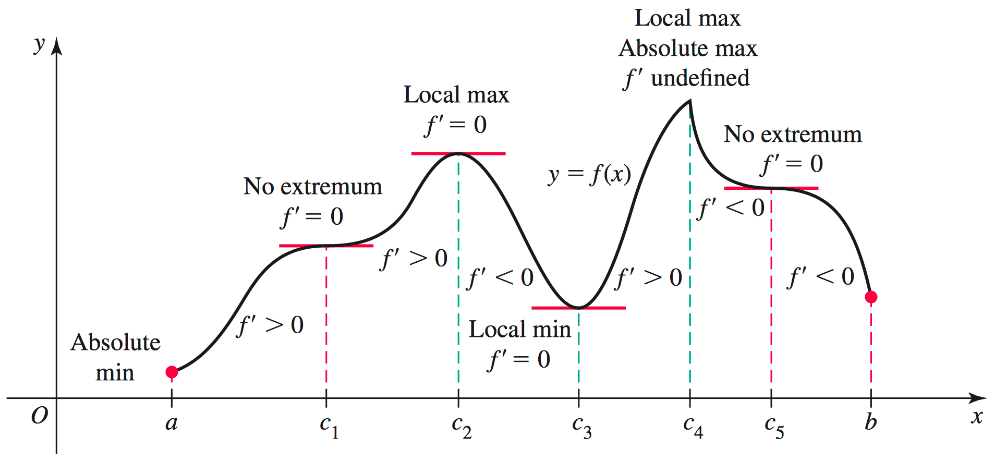
\includegraphics[width=0.85\linewidth]{images/briggs_04_03/fig4_27.png}
\end{center}
\vspace*{\stretch{1}}
\begin{center}
  \begin{tabularx}{0.95\linewidth}{*{3}{X}}\toprule
    $f(x)$& $f'(x)$& $f''(x)$\\\midrule
    increasing& positive& ---\\
    decreasing& negative& ---\\
%    max& crit. pt. \& changes sign& ---\\
    max/min& crit. pt. \& changes sign& ---\\
    concave up& increasing& positive\\
    concave down& decreasing& negative\\
    Inflection point& max/min& crit. pt. \& changes sign\\\bottomrule
  \end{tabularx}
\end{center}
\vspace*{\stretch{1}}
\pagebreak

\noindent
\fbox{\parbox{0.9875\linewidth}{
  \textbf{Theorem 4.11: Second Derivative Test for Local Extrema}
  
  Suppose $f''$ is continuous on an open interval containing $c$ with $f'(c)=0$.
  \begin{itemize}
    \item If $f''(c)>0$, then $f$ has a local minimum at $c$ (Figure 4.40a).
    \item If $f''(c)<0$, then $f$ has a local maximum at $c$  (Figure 4.40b).
    \item If $f''(c)=0$, then the test is inconclusive; $f$ may have a local maximum, local minimum, or neither at $c$.
  \end{itemize}
}}

\begin{center}
  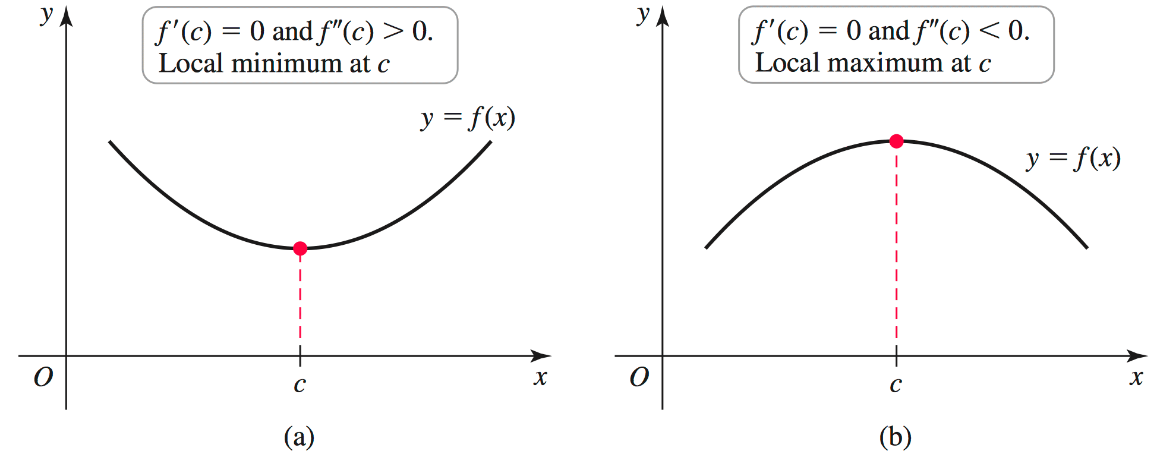
\includegraphics[width=0.8\linewidth]{images/briggs_04_03/fig4_40.png}
\end{center}
\begin{ex*}
  For each of the following, use the Second Derivative Test for Extrema to determine local max/mins:
\end{ex*}
\begin{tasks}(3)
  \task $f(x)=x^5-5x+3$
  \task $f(x)=2x^3-3x^2+12$
  \task $f(x)=x^3-6$
\end{tasks}
\pagebreak
\vspace*{\stretch{1}}
\begin{center}
  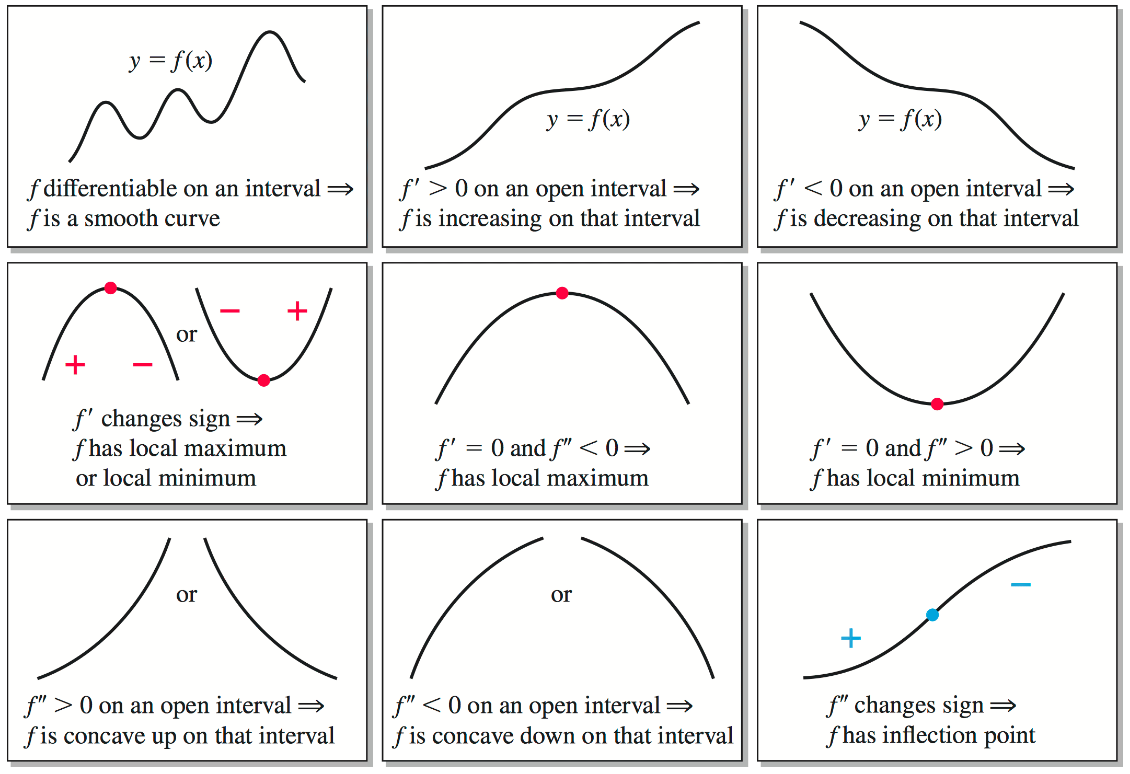
\includegraphics[width=1.0\linewidth]{images/briggs_04_03/fig4_43.png}
\end{center}
\vspace*{\stretch{1}}
\pagebreak

\end{document}

\documentclass[answers]{exam}
\usepackage{texPreamble}
\usepackage{relsize}
\usepackage{tabularx}
\extraheadheight{0.25in}
\extrafootheight{1.0in}
\extrawidth{1in}
% ----------------------------------------------------------------
\firstpagefootrule
\runningfootrule
\begin{document}
%\relscale{1.4}
\section{4.4: Graphing Functions}
\noindent
\fbox{\parbox{0.9875\linewidth}{
  \textbf{Graphing Guidelines for } $y=f(x)$
  
  \parbox{0.9\linewidth}{
  \begin{enumerate}
    \item Identify the domain or interval of interest.
    \item Determine if the function is symmetric.
    \item Use $f'(x)$ and $f''(x)$ to determine 
      \begin{itemize}
        \item intervals of increasing/decreasing\dotfill $f'(x)>0$ or $f'(x)<0$
        \item relative max/mins\dotfill 1st or 2nd derivative test
        \item concave up/concave down\dotfill $f''(x)>0$ or $f''(x)<0$
        \item inflection points\dotfill $f''(x)$ changes signs
      \end{itemize}
    \item Find asymptotes
      \begin{itemize}
        \item vertical\dotfill $\lim_{x\to a} f(x)=\pm\infty$
        \item horizontal\dotfill $\lim_{x\to \pm\infty} f(x)=c$
        \item slant\dotfill $y=ax+b$
      \end{itemize}
    \item Intercepts
      \begin{itemize}
        \item $y$-intercept\dotfill evaluate $f(0)$
        \item $x$-intercept\dotfill solve $f(x)=0$
      \end{itemize}
    \item Sketch using the characteristics found above
  \end{enumerate}}
}}
\pagebreak
\begin{ex*}
  Sketch the following functions using derivatives:
\end{ex*}

\begin{enumerate}
  \item $f(x)=x^4-6x^2$ 
    \vspace*{\stretch{1}}
    \begin{flushright}
      \begin{tikzpicture}
        \begin{axis}[
          axis lines=center,
          axis line style={->},
          xmin=-3, xmax=3,
          ymin=-6, ymax=6,
          xtick={-8,-6,...,8},
%          ytick={-6,-5,...,6},
%          xmajorticks=false,
          ymajorticks=false,
          minor x tick num=1,
%          minor y tick num=3,
          enlargelimits={abs=0.75},
          width=0.5\linewidth,
          ticklabel style={font=\footnotesize,inner sep=0.5pt,fill=white,opacity=1.0, text opacity=1},
          xlabel=$x$, xlabel style={at={(ticklabel* cs:1)},anchor=north west},
          ylabel=$y$, ylabel style={at={(ticklabel* cs:1)},anchor=south west},
          every axis plot/.append style={line width=0.95pt, color=blue, samples=100}
          ]
        \end{axis}
      \end{tikzpicture}
    \end{flushright}
    \pagebreak
  \item $g(x)=200+8x^3+x^4$ 
    \vspace*{\stretch{1}}
    \begin{flushright}
      \begin{tikzpicture}
        \begin{axis}[
          axis lines=center,
          axis line style={->},
          xmin=-9, xmax=9,
          ymin=-6, ymax=6,
          xtick={-8,-6,...,8},
%          ytick={-6,-5,...,6},
%          xmajorticks=false,
          ymajorticks=false,
          minor x tick num=1,
%          minor y tick num=3,
          enlargelimits={abs=0.75},
          width=0.5\linewidth,
          ticklabel style={font=\footnotesize,inner sep=0.5pt,fill=white,opacity=1.0, text opacity=1},
          xlabel=$x$, xlabel style={at={(ticklabel* cs:1)},anchor=north west},
          ylabel=$y$, ylabel style={at={(ticklabel* cs:1)},anchor=south west},
          every axis plot/.append style={line width=0.95pt, color=blue, samples=100}
          ]
        \end{axis}
      \end{tikzpicture}
    \end{flushright}
    \pagebreak
  \item $y=\dfrac{x}{(x-1)^2}$ 
    \vspace*{\stretch{1}}
    \begin{flushright}
      \begin{tikzpicture}
        \begin{axis}[
          axis lines=center,
          axis line style={->},
          xmin=-3, xmax=3,
          ymin=-1, ymax=1,
          xtick={-2,0,...,2},
          ytick={-1,0,...,1},
%          xmajorticks=false,
%          ymajorticks=false,
          minor x tick num=1,
%          minor y tick num=3,
          enlargelimits={abs=0.75},
          width=0.5\linewidth,
          ticklabel style={font=\footnotesize,inner sep=0.5pt,fill=white,opacity=1.0, text opacity=1},
          xlabel=$x$, xlabel style={at={(ticklabel* cs:1)},anchor=north west},
          ylabel=$y$, ylabel style={at={(ticklabel* cs:1)},anchor=south west},
          every axis plot/.append style={line width=0.95pt, color=blue, samples=100}
          ]
        \end{axis}
      \end{tikzpicture}
    \end{flushright}
    \pagebreak
  \item $y=\dfrac{x^2-4}{x^2-2x}$ 
    \vspace*{\stretch{1}}
    \begin{flushright}
      \begin{tikzpicture}
        \begin{axis}[
          axis lines=center,
          axis line style={->},
          xmin=-4, xmax=4,
          ymin=-4, ymax=4,
          xtick={-4,-3,...,4},
          ytick={-4,-3,...,4},
          xticklabels={,,},
          yticklabels={,,},
%          xmajorticks=false,
%          ymajorticks=false,
%          minor x tick num=1,
%          minor y tick num=3,
          enlargelimits={abs=0.75},
          width=0.5\linewidth,
          ticklabel style={font=\footnotesize,inner sep=0.5pt,fill=white,opacity=1.0, text opacity=1},
          xlabel=$x$, xlabel style={at={(ticklabel* cs:1)},anchor=north west},
          ylabel=$y$, ylabel style={at={(ticklabel* cs:1)},anchor=south west},
          every axis plot/.append style={line width=0.95pt, color=blue, samples=100}
          ]
        \end{axis}
      \end{tikzpicture}
    \end{flushright}
    \pagebreak
  \item $f(x)=\dfrac{(x+1)^3}{(x-1)^2}$ 
    \vspace*{\stretch{1}}
    \begin{flushright}
      \begin{tikzpicture}
        \begin{axis}[
          axis lines=center,
          axis line style={->},
          xmin=-8, xmax=8,
          ymin=-22, ymax=22,
          xtick={-8,-4,...,8},
          ytick={-20,-15,...,20},
%         xmajorticks=false,
%         ymajorticks=false,
          minor x tick num=3,
%          minor y tick num=3,
          enlargelimits={abs=0.75},
          width=0.5\linewidth,
          ticklabel style={font=\footnotesize,inner sep=0.5pt,fill=white,opacity=1.0, text opacity=1},
          xlabel=$x$, xlabel style={at={(ticklabel* cs:1)},anchor=north west},
          ylabel=$y$, ylabel style={at={(ticklabel* cs:1)},anchor=south west},
          every axis plot/.append style={line width=0.95pt, color=blue, samples=100}
          ]
        \end{axis}
      \end{tikzpicture}
    \end{flushright}
    \pagebreak
  \item $y=\dfrac{x^2}{x^2+3}$ 
    \vspace*{\stretch{1}}
    \begin{flushright}
      \begin{tikzpicture}
        \begin{axis}[
          axis lines=center,
          axis line style={->},
          xmin=-4.5, xmax=4.5,
          ymin=-0.1, ymax=1.2,
          xtick={-4,-2,...,4},
          ytick={-4,-3,...,4},
%          xmajorticks=false,
%          ymajorticks=false,
          minor x tick num=1,
          minor y tick num=3,
%          enlargelimits={abs=0.5},
          width=0.5\linewidth,
          ticklabel style={font=\footnotesize,inner sep=0.5pt,fill=white,opacity=1.0, text opacity=1},
          xlabel=$x$, xlabel style={at={(ticklabel* cs:1)},anchor=north west},
          ylabel=$y$, ylabel style={at={(ticklabel* cs:1)},anchor=south west},
          every axis plot/.append style={line width=0.95pt, color=blue, samples=100}
          ]
        \end{axis}
      \end{tikzpicture}
    \end{flushright}
    \pagebreak
  \item $f(x)=\dfrac{x^3}{(x+1)^2}$ 
    \vspace*{\stretch{1}}
    \begin{flushright}
      \begin{tikzpicture}
        \begin{axis}[
          axis lines=center,
          axis line style={->},
          xmin=-8, xmax=8,
          ymin=-6, ymax=6,
          xtick={-8,-7,...,8},
          ytick={-6,-5,...,6},
          xticklabels={,,},
          yticklabels={,,},
%          xmajorticks=false,
%          ymajorticks=false,
%          minor x tick num=1,
%          minor y tick num=3,
          enlargelimits={abs=0.75},
          width=0.5\linewidth,
          ticklabel style={font=\footnotesize,inner sep=0.5pt,fill=white,opacity=1.0, text opacity=1},
          xlabel=$x$, xlabel style={at={(ticklabel* cs:1)},anchor=north west},
          ylabel=$y$, ylabel style={at={(ticklabel* cs:1)},anchor=south west},
          every axis plot/.append style={line width=0.95pt, color=blue, samples=100}
          ]
        \end{axis}
      \end{tikzpicture}
    \end{flushright}
    \pagebreak
  \item $y=x^{1/5}$ 
    \vspace*{\stretch{1}}
    \begin{flushright}
      \begin{tikzpicture}
        \begin{axis}[
          axis lines=center,
          axis line style={->},
          xmin=-1, xmax=1,
          ymin=-1, ymax=1,
%          xtick={-3,-2,...,2},
%          ytick={-4,-3,...,4},
          xmajorticks=false,
          ymajorticks=false,
%          minor x tick num=1,
%          minor y tick num=3,
          enlargelimits={abs=0.75},
          width=0.5\linewidth,
          ticklabel style={font=\footnotesize,inner sep=0.5pt,fill=white,opacity=1.0, text opacity=1},
          xlabel=$x$, xlabel style={at={(ticklabel* cs:1)},anchor=north west},
          ylabel=$y$, ylabel style={at={(ticklabel* cs:1)},anchor=south west},
          every axis plot/.append style={line width=0.95pt, color=blue, samples=100}
          ]
        \end{axis}
      \end{tikzpicture}
    \end{flushright}
    \pagebreak
  \item $y=2\sqrt x-x$ 
    \vspace*{\stretch{1}}
    \begin{flushright}
      \begin{tikzpicture}
        \begin{axis}[
          axis lines=center,
          axis line style={->},
          xmin=-1, xmax=8,
          ymin=-1, ymax=1,
          xtick={-3,-2,...,8},
          ytick={-4,-3,...,8},
          xticklabels={,,},
%          xmajorticks=false,
%          ymajorticks=false,
%          minor x tick num=1,
%          minor y tick num=3,
          enlargelimits={abs=0.75},
          width=0.5\linewidth,
          ticklabel style={font=\footnotesize,inner sep=0.5pt,fill=white,opacity=1.0, text opacity=1},
          xlabel=$x$, xlabel style={at={(ticklabel* cs:1)},anchor=north west},
          ylabel=$y$, ylabel style={at={(ticklabel* cs:1)},anchor=south west},
          every axis plot/.append style={line width=0.95pt, color=blue, samples=100}
          ]
        \end{axis}
      \end{tikzpicture}
    \end{flushright}
    \pagebreak
  \item $y=\dfrac{1}{1+e\inv[x]}$ 
    \vspace*{\stretch{1}}
    \begin{flushright}
      \begin{tikzpicture}
        \begin{axis}[
          axis lines=center,
          axis line style={->},
          xmin=-3, xmax=3,
          ymin=0, ymax=1,
          xtick={-3,-2,...,2},
          ytick={-4,-3,...,4},
          xmajorticks=false,
%          ymajorticks=false,
%          minor x tick num=1,
%          minor y tick num=3,
          enlargelimits={abs=0.25},
          width=0.5\linewidth,
          ticklabel style={font=\footnotesize,inner sep=0.5pt,fill=white,opacity=1.0, text opacity=1},
          xlabel=$x$, xlabel style={at={(ticklabel* cs:1)},anchor=north west},
          ylabel=$y$, ylabel style={at={(ticklabel* cs:1)},anchor=south west},
          every axis plot/.append style={line width=0.95pt, color=blue, samples=100}
          ]
        \end{axis}
      \end{tikzpicture}
    \end{flushright}
    \pagebreak
  \item $f(x)=\dfrac{x^2}{x^2-4}$ 
    \vspace*{\stretch{1}}
    \begin{flushright}
      \begin{tikzpicture}
        \begin{axis}[
          axis lines=center,
          axis line style={->},
          xmin=-4, xmax=4,
          ymin=-3, ymax=3,
          xtick={-2,2},
          ytick={-4,-3,...,4},
          yticklabels={,,},
%          xmajorticks=false,
%          ymajorticks=false,
%          minor x tick num=1,
%          minor y tick num=3,
          enlargelimits={abs=0.75},
          width=0.5\linewidth,
          ticklabel style={font=\footnotesize,inner sep=0.5pt,fill=white,opacity=1.0, text opacity=1},
          xlabel=$x$, xlabel style={at={(ticklabel* cs:1)},anchor=north west},
          ylabel=$y$, ylabel style={at={(ticklabel* cs:1)},anchor=south west},
          every axis plot/.append style={line width=0.95pt, color=blue, samples=100}
          ]
        \end{axis}
      \end{tikzpicture}
    \end{flushright}
\end{enumerate}
\pagebreak

\begin{ex*}
  Using the following derivatives, sketch a possible graph of the original function.
\end{ex*}
\begin{enumerate}[itemsep=\stretch{1}]
  \item $f'(x)=\dfrac{1}{6}(x+1)(x-2)^2(x-3)$ 
    \vspace*{\stretch{1}}
    \begin{flushright}
      \begin{tikzpicture}
        \begin{axis}[
          axis lines=center,
          axis line style={->},
          xmin=-3, xmax=3,
          ymin=0, ymax=1,
          xtick={-3,-2,...,2},
          ytick={-4,-3,...,4},
%          xmajorticks=false,
          ymajorticks=false,
%          minor x tick num=1,
%          minor y tick num=3,
          enlargelimits={abs=0.25},
          width=0.5\linewidth,
          ticklabel style={font=\footnotesize,inner sep=0.5pt,fill=white,opacity=1.0, text opacity=1},
          xlabel=$x$, xlabel style={at={(ticklabel* cs:1)},anchor=north west},
          ylabel=$y$, ylabel style={at={(ticklabel* cs:1)},anchor=south west},
          every axis plot/.append style={line width=0.95pt, color=blue, samples=100}
          ]
        \end{axis}
      \end{tikzpicture}
    \end{flushright}
  \item $g'(x)=x^2(x+2)(x-1)$
    \vspace*{\stretch{1}}
    \begin{flushright}
      \begin{tikzpicture}
        \begin{axis}[
          axis lines=center,
          axis line style={->},
          xmin=-3, xmax=3,
          ymin=0, ymax=1,
          xtick={-3,-2,...,2},
          ytick={-4,-3,...,4},
%          xmajorticks=false,
          ymajorticks=false,
%          minor x tick num=1,
%          minor y tick num=3,
          enlargelimits={abs=0.25},
          width=0.5\linewidth,
          ticklabel style={font=\footnotesize,inner sep=0.5pt,fill=white,opacity=1.0, text opacity=1},
          xlabel=$x$, xlabel style={at={(ticklabel* cs:1)},anchor=north west},
          ylabel=$y$, ylabel style={at={(ticklabel* cs:1)},anchor=south west},
          every axis plot/.append style={line width=0.95pt, color=blue, samples=100}
          ]
        \end{axis}
      \end{tikzpicture}
    \end{flushright}
\end{enumerate}
\pagebreak

%TODO remove relscale
\end{document}

\documentclass[answers]{exam}
\usepackage{texPreamble}
\usepackage{relsize}
\usepackage{tabularx}
\extraheadheight{0.25in}
\extrafootheight{1.0in}
\extrawidth{1in}
% ----------------------------------------------------------------
\firstpagefootrule
\runningfootrule
\begin{document}
%\relscale{1.4}
\section{4.6: Linear Approximation and Differentials}
\begin{ex*}
  Find the equation of the line tangent to $f(x)=1+\sin(x)$ at $a=0$. State the line in the slope--intercept form.
\end{ex*}
\vspace*{\stretch{1}}
\begin{flushright}
  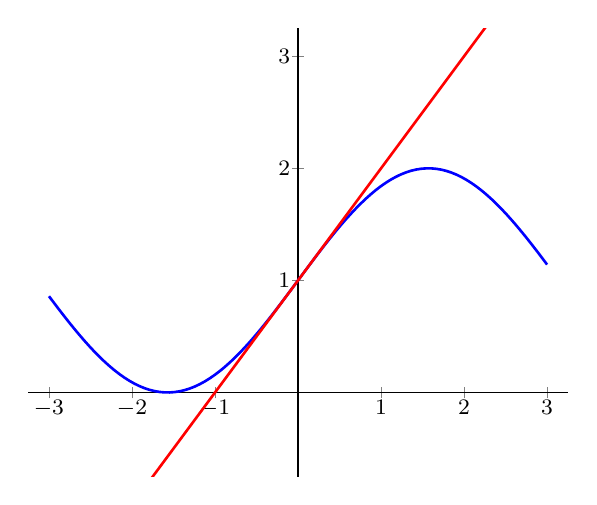
\begin{tikzpicture}
    \begin{axis}[
      grid style={line width=0.35pt, draw=gray!75},
      axis lines=center,
      axis line style={-},
      xmin=-3.25, xmax=3.25,
      ymin=-0.75, ymax=3.25,
      xtick={-6,-5,...,6},
      ytick={-6,-5,...,6},
      ticklabel style={font=\footnotesize,inner sep=0.5pt,fill=white,opacity=1.0, text opacity=1},
      every axis plot/.append style={line width=0.95pt, color=blue, samples=100}
      ]
      \addplot[-] expression[domain=-3:3]{1+sin(deg(x))};
      \addplot[-] expression[red]{x+1};
    \end{axis}
  \end{tikzpicture}
\end{flushright}
\begin{defn*}
  \textbf{Linear Approximation of $f$ at $a$.}
  
  Suppose $f$ if differentiable on an interval $I$ containing the point $a$. The \textbf{linear approximation} to $f$ at $a$ is the linear function.
  
  $$L(x)=f(a)+f'(a)(x-a),\ \textnormal{ for } x \textnormal{ in } I.$$
\end{defn*}
\pagebreak

\begin{ex*}
  Consider the function $f(x)=\dfrac{x}{x+1}$. Find the linearization at $a=1$. Use the linearization to estimate $f(1.1)$ and compare with the true value of $f(1.1)$.
\end{ex*}
\vspace*{\stretch{1}}

\begin{ex*}
  Find the linearization $L(x)$ of $f(x)=e^{3x-6}$ at $a=2$.
\end{ex*}
\vspace*{\stretch{1}}

\begin{ex*}
  Find the linearization $L(x)$ of $f(x)=9\parens{4x+11}^\frac{2}{3}$ at $a=4$.
\end{ex*}
\vspace*{\stretch{1}}

\pagebreak
\begin{ex*}
  Find a linearization over an interval which will contain the given point $x_0$. Choose your center at a point \textit{near} $x_0$ but not at $x_0$ so that the given function and its derivative are easy to evaluate. Lastly, use the linearization to approximate $f(x_0)$.
\end{ex*}
\begin{enumerate}[label=\alph*), itemsep=\stretch{1}]
  \item $f(x)=x^2+2x,\ x_0=0.1$
  \item $f(x)=\sqrt[3]{x},\ x_0=8.5$.
\end{enumerate}
\vspace*{\stretch{1}}
\pagebreak

\begin{ex*}
  Use a linear approximation to estimate $\sqrt{146}$.
\end{ex*}
\vspace*{\stretch{1}}

\begin{ex*}
  Use a linear approximation to estimate $\parens{1.999}^4$.
\end{ex*}
\vspace*{\stretch{1}}

\begin{ex*}
  Use a linear approximation to estimate $\sqrt{\dfrac{5}{29}}$.
\end{ex*}
\vspace*{\stretch{1}}
\pagebreak

\begin{ex*}
  Find the linearization $L(x)$ of $f(x)=\sqrt{x^2+9}$ at $a=-4$. Use $L(x)$ to estimate $f(-4.1)$ and $\sqrt{23.44}$. (\textit{Hint:} $3.8^2=14.44$)
\end{ex*}
\vspace*{\stretch{1}}
  
\begin{ex*}
  Use a linearization to show that $0.05$ is a good approximation for $\ln(1.05)$.
\end{ex*}
\vspace*{\stretch{1}}
\pagebreak
\noindent
\fbox{\parbox{0.9875\linewidth}{
  \textbf{Concavity and Overestimating versus Underestimating.} Suppose $L(x)$ is a linearization of $f(x)$ centered at $a$.
  \begin{enumerate}
    \item
        If $f''(a)>0$, then $L(x)$ is an underestimation of $f$.
    \item 
        If $f''(a)<0$, then $L(x)$ is an overestimation of $f$.
  \end{enumerate}
}}
\begin{center}
    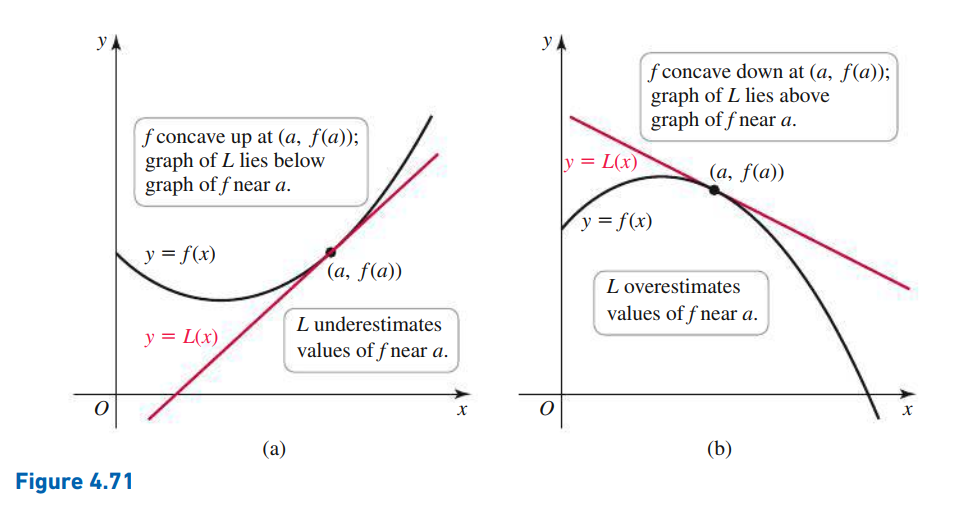
\includegraphics[scale=0.5]{images/briggs_04_06/fig4_71}
\end{center}

\begin{ex*}
  Find the linearization of the following functions at the given point and use concavity to identify if the linearization is an overestimate or an underestimate.
\end{ex*}
\begin{enumerate}[label=\alph*),itemsep=\stretch{1}]
  \item $f(x)=\dfrac{2}{x};\, a=1$
  \item $f(x)=e\inv[x];\, a=\ln(2)$
\end{enumerate}
\vspace*{\stretch{1}}
\pagebreak

%\noindent
%\fbox{\parbox{0.9875\linewidth}{
%  \textbf{Summary: Uses of Linear Approximation}
%  \begin{enumerate}
%    \item 
%      To approximate $f$ near $x=a$, use
%        $$f(x)\approx L(x)=f(a)+f'(a)(x-a).$$
%    \item 
%      To approximate the change $\Delta y$ in the dependent variable when the independent variable $x$ changes from $a$ to $a+\Delta x$, use
%        $$\Delta y\approx f'(a)\Delta x.$$
%  \end{enumerate}
%}}
%\pagebreak

%\begin{defn*}[Differentials]
%  
%  Let $f$ be differentiable on an interval containing $x$. A small change in $x$ is denoted by the \textbf{differential} $dx$. The corresponding change in $f$ is approximated by the \textbf{differential} $dy=f'(x)\,dx$. So if $\Delta x=dx$, where $\Delta x$ and $dx$ are both small, then $\Delta y\approx dy$:
%    \[\Delta y= f(x+dx)-f(x)\approx dy=f'(x)\,dx.\]
%    
%\end{defn*}

\begin{defn*}[Differentials]
    Let $f$ be a differentiable function on an interval containing $x$. An infinitesimal change in $x$ can be denoted by the \textbf{differential} $dx$. The corresponding change in the output of $f$ can be denoted by the \textbf{differential} $dy$. This yields the relation
        $$dy = f'(x)dx.$$
    Note that $dy$ and $dx$ can be thought of as the `rise' and `run' (respectively) of the line tangent to $f$ at the point $(x,f(x))$.
\end{defn*}

\begin{defn*}[$\Delta x$ and $\Delta y$]
    Let $f$ be a differentiable function on an interval containing $x$. We let $\Delta x$ denote a small change in $x$ and we let $\Delta y$ denote the corresponding change in $f(x)$. This yields the relation
        $$\Delta y = f(x+\Delta x) - f(x).$$
    Note that $\Delta y$ and $\Delta x$ can be thought of as the `rise' and `run' (respectively) of the secant line passing through the points $(x,f(x))$ and $(x+\Delta x, f(x+\Delta x))$.
\end{defn*}

\vspace*{\stretch{1}}
\noindent
\fbox{\parbox{0.9875\linewidth}{
  \textbf{Linear Approximation and Differentials}
    To approximate the change $\Delta y$ in the dependent variable when the independent variable $x$ changes from $x$ to $x+\Delta x$, use
        $$\Delta y\approx f'(x)\Delta x$$
    because if we set $\Delta x = dx$, then we have the following:
        $$\Delta y= f(x+\Delta x)-f(x)\approx f'(x)\,dx=dy.$$
    One can think of $\Delta y$ as the \textit{actual change} in the output of a function when $x$ changes by $\Delta x$, whereas $f'(x)\Delta x$ is the \textit{projected change} in the output of the function when the same $\Delta x$ is imposed. The point is these are approximately equal when $\Delta x$ is small.
}}
\vspace*{\stretch{1}}
\pagebreak

\begin{ex*}
  Find the differential $dy$.
\end{ex*}
\begin{tasks}[after-item-skip=\stretch{1}, label=~](2)
  \task $y=\cos(x^2)$
  \task $y=\sqrt{1-x^2}$
  \task $y=4x^2-3x+2$
  \task $y=x\tan(x^3)$
  \task $y=\cos^5(x)$
  \task $f(x)=\sin\inv(x)$
\end{tasks}
\vspace*{\stretch{1}}
\pagebreak
\begin{ex*}
  Let $y=x^2$
\end{ex*}
\begin{enumerate}[label=\alph*), itemsep=\stretch{1}]
  \item Find $dy$
  \item If $x=1$ and $dx=0.01$, find $dy$.
  \item Compare $dy$ and $\Delta y$ at this point.
\end{enumerate}
\vspace*{\stretch{1}}

\begin{ex*}
  Let $y=\sqrt{3+x^2}$
\end{ex*}
\begin{enumerate}[label=\alph*), itemsep=\stretch{1}]
  \item Find $dy$
  \item If $x=1$ and $dx=-0.1$, find $dy$.
  \item Compare $dy$ and $\Delta y$ at this point.
\end{enumerate}
\vspace*{\stretch{1}}

\pagebreak
\begin{ex*}
  Suppose $f$ is differentiable on $(-\infty,\infty)$ and $f(5.01)-f(5)=0.25$. Use linear approximation to estimate the value of $f'(5)$.
\end{ex*}
\vspace*{\stretch{1}}

\begin{ex*}
  Suppose $f$ is differentiable on $(-\infty,\infty)$ and $f(5.99)=7$ and $f(6)=7.002$. Use linear approximation to estimate the value of $f'(6)$.
\end{ex*}
\vspace*{\stretch{1}}
\pagebreak

\begin{ex*}
  Compute $dy$ and $\Delta y$ for $y=e^x$ when $x=0$ and $\Delta x=0.5$.
\end{ex*}
\vspace*{\stretch{1}}

\begin{ex*}
  Approximate the change in the area of a circle when its radius increases from $2.00$ to $2.02\,m$.
\end{ex*}
\vspace*{\stretch{1}}

\begin{ex*}
  Approximate the change in the magnitude of the electrostatic force between two charges when the distance between them increases from $r=20\,m$ to $r=21\,m$ $(F(r)=0.01/r^2$).
\end{ex*}
\vspace*{\stretch{1}}
\pagebreak

\begin{ex*}
  Approximate the change in the volume of a right circular cylinder of fixed radius $r=20\,cm$ when its height decreases from $h=12\,cm$ to $h=11.9\,cm$ ($V(h)=\pi r^2h$).
\end{ex*}
\vspace*{\stretch{1}}

\begin{ex*}
  Approximate the change in the volume of a right circular cylinder of fixed height $h=4\,m$ when its radius increases from $r=3\,m$ to $r=3.05\,m$ ($V(r)=\frac{1}{3}\pi r^2 h$).
\end{ex*}
\vspace*{\stretch{1}}
\pagebreak

\begin{ex*}
  The radius of a sphere is measured and found to be $0.7$ inches with a possible error in measurement of at most 0.01 inches.
\end{ex*}
\begin{enumerate}[label=\alph*), itemsep=\stretch{1}]
  \item What is the maximum error in using the value of the radius to compute the volume of the sphere?
  \item Find the relative error of the volume: \hfill\textit{relative error} $\dfrac{dV}{V}$\hspace*{50pt}
  
  What is the percentage error?
\end{enumerate}
\vspace*{\stretch{1}}
\pagebreak

\begin{ex*}
  The radius of a circular disk is given as $24\,cm$ with a maximum error in measurement of $0.2\,cm$.
\end{ex*}
\begin{enumerate}[label=\alph*), itemsep=\stretch{1}]
  \item Use differentials to estimate the maximum error in the calculated area of the disk.
  \item What is the relative error? What is the percentage error?
\end{enumerate}
\vspace*{\stretch{1}}
\pagebreak

\begin{ex*}
  Use differentials to estimate the amount of paint needed to apply a coat of paint $0.05\,cm$ thick to a hemispherical dome with diameter $50\,m$.
\end{ex*}
\vspace*{\stretch{1}}
\pagebreak
\end{document}

\documentclass[answers]{exam}
\usepackage{texPreamble}
\usepackage{relsize}
\usepackage{tabularx}
\extraheadheight{0.25in}
\extrafootheight{1.0in}
\extrawidth{1in}
% ----------------------------------------------------------------
\firstpagefootrule
\runningfootrule
\begin{document}
%\relscale{1.4}
\section{4.7: L'H\^ opital's Rule}
\noindent
\fbox{\parbox{0.9875\linewidth}{
  \textbf{Theorem 4.12: L'H\^opital's Rule}
  
  Suppose $f$ and $g$ are differentiable on an open interval $I$ containing $a$ with $g'(x)\neq 0$ on $I$ when $x\neq a$. If $\ds\lim_{x\to a} f(x)=\lim_{x\to a} g(x)=0$, then
    \[\lim_{x\to a}\frac{f(x)}{g(x)}=\lim_{x\to a}\frac{f'(x)}{g'(x)}\]
  provided the limit on the right exists (or is $\pm\infty$). The rule also applies if $x\to a$ is replaced with $x\to\pm\infty$, $x\to a^+$, or $x\to a\inv[]$.
}}

\vspace*{10pt}

\noindent
\fbox{\parbox{0.9875\linewidth}{
  \textbf{Theorem 4.13: L'H\^opital's Rule $(\infty/\infty)$}
  
  Suppose $f$ and $g$ are differentiable on an open interval $I$ containing $a$ with $g'(x)\neq 0$ on $I$ when $x\neq a$. If $\ds\lim_{x\to a} f(x)= \pm\infty$ and $\lim_{x\to a} g(x)=\pm\infty$, then
    \[\lim_{x\to a}\frac{f(x)}{g(x)}=\lim_{x\to a}\frac{f'(x)}{g'(x)}\]
  provided the limit on the right exists (or is $\pm\infty$). The rule also applies for $x\to\pm\infty$, $x\to a^+$, or $x\to a\inv[]$.
}}

\vspace*{5pt}
\hspace*{\stretch{1}}
\textit{Note:} Limits of the form $\dfrac{0}{0}$ and $\dfrac{\infty}{\infty}$ are called \textit{indeterminate forms}.
\hspace*{\stretch{1}}

\noindent\hrulefill

\textbf{Notes on grading:}
\begin{enumerate}
  \item Unless specifically told to use L'H\^opital's Rule, you may use any valid method to evaluate limits.
  \item Remember to 
    \begin{enumerate}
      \item keep your limit notation until the direct substitution step
      \item connect each step with equal signs
      \item notate the equal signs where L'H\^opital is used
    \end{enumerate}
  \item L'H\^opital does NOT replace the quotient rule!
\end{enumerate}

\pagebreak

\begin{ex*}
  Find the following limits with and without L'H\^opital's Rule:
\end{ex*}
\begin{tasks}[after-item-skip=\stretch{1}, label=~](2)
  \task 
    $\ds\lim_{x\to 2} \frac{x^2-4}{x-2}$
  \task 
    $\ds\lim_{x\to \infty} \frac{2x^2+3x}{x^3+x+1}$
\end{tasks}
\vspace*{\stretch{1}}

\hspace*{\stretch{1}}
\fbox{\parbox{0.675\linewidth}{\centering
\textit{Note:} L'H\^opital's Rule only works for indeterminate forms!}}
\hspace*{\stretch{1}}

\begin{ex*}
  Find the following limit with and without L'H\^opital's Rule:
\end{ex*}
\begin{tasks}[after-item-skip=\stretch{1}, label=~](1)
  \task $\ds\lim_{x\to \frac{\pi}{2}} \frac{\sin(x)}{1-\cos(x)}$
\end{tasks}
\vspace*{\stretch{1}}
\pagebreak

\begin{ex*}
  Find the following limits:
\end{ex*}
\begin{tasks}[after-item-skip=\stretch{1}, label=~](2)
  \task 
    $\ds\lim_{t\to 1} \frac{t^3-1}{4t^3-t-3}$
  \task 
    $\ds\lim_{z\to 0} \frac{\tan(4z)}{\tan(7z)}$
\end{tasks}
\vspace*{\stretch{1}}
\begin{ex*}
  Find the following limits. Repeat L'H\^opital's Rule each time you get an indeterminate form:
\end{ex*}
\begin{tasks}[after-item-skip=\stretch{1}, label=~](1)
  \task 
    $\ds\lim_{x\to 0} \frac{\sin(x)-x}{x^3}$
  \task 
    $\ds\lim_{t\to 0} \frac{t\sin(t)}{1-\cos(t)}$
\end{tasks}
\vspace*{\stretch{1}}
\pagebreak

\begin{ex*}
  Evaluate:
\end{ex*}
\begin{tasks}[after-item-skip=\stretch{1}, label=~](2)
  \task $\ds\lim_{x\to 0^+} \frac{\ln(x)}{x}$
  \task $\ds\lim_{x\to 3} \frac{2x^2-5x+1}{x^2+x-6}$
  \task $\ds\lim_{x\to \frac{1}{2}} \frac{6x^2+5x-4}{4x^2+16x-9}$
  \task $\ds\lim_{x\to \infty} \frac{x-8x^2}{12x^2+5x}$
  \task $\ds\lim_{t\to 0} \frac{e^{2t}-1}{\sin(t)}$
  \task $\ds\lim_{t\to 0} \frac{8^t-5^t}{t}$ 
\end{tasks}
\vspace*{\stretch{1}}
\pagebreak
\noindent

\hspace*{\stretch{1}}
\fbox{\parbox{0.675\linewidth}{\centering
\textit{Note:} $0\cdot \infty$ and $\infty-\infty$ are also indeterminate forms.

L'H\^opital's Rule can be used after these functions are converted into rational functions of indeterminate form.
}}
\hspace*{\stretch{1}}

\begin{ex*}
  Find the following limits. Convert into indeterminate form as needed:
\end{ex*}
\begin{tasks}[after-item-skip=\stretch{1}, label=~](1)
  \task $\ds\lim_{x\to 1\inv[]}(1-x)\tan\parens{\frac{\pi x}{2}}$
  \task $\ds\lim_{x\to \infty} x^2\sin\parens{\frac{1}{4x^2}}$
  \task $\ds\lim_{x\to 0^+} \parens{\csc(x)-\cot(x)+\cos(x)}$
\end{tasks}
\vspace*{\stretch{1}}
\pagebreak

\fbox{\parbox{0.9875\linewidth}{
  \textbf{Indeterminate forms $1^\infty$, $0^0$, and $\infty^0$.}
  
  Assume $\ds\lim_{x\to a} f(x)^{g(x)}$ has the indeterminate form $1^\infty$, $0^0$, or $\infty^0$.
  \begin{enumerate}
    \item Analyze $L=\ds\lim_{x\to a} g(x)\ln\parens{f(x)}$. This limit can be put in the form $0/0$ or $\infty/\infty$, both of which are handled by L'H\^opital's Rule.
    \item When $L$ is finite, $\ds\lim_{x\to a} f(x)^{g(x)}= e^L$. If $L=\infty$ or $L=-\infty$, then \newline$\ds\lim_{x\to a} f(x)^{g(x)}=\infty$ or $\ds\lim_{x\to a} f(x)^{g(x)}=0$, respectively.
  \end{enumerate}
  
  \textit{Note:} $0^\infty$ and $\infty^\infty$ are NOT indeterminate forms.
}}

\begin{tasks}[after-item-skip=\stretch{1}, label=~](2)
  \task $\ds\lim_{x\to 0^+} x^{-1/\ln(x)}$
  \task $\ds\lim_{x\to \infty} (1+2x)^{1/(2\ln(x))}$
\end{tasks}
\vspace*{\stretch{1}}
\pagebreak

\noindent
When working with the exponential indeterminate forms, the transformations are typically very similar:
\begin{center}
  \renewcommand{\arraystretch}{1.5}
  {\begin{tabular}{@{}lL|*{3}{R}@{}}
    \multicolumn{2}{@{}c}{}&\multicolumn{3}{c@{}}{Indeterminate form}\\
    \multirow{3}{*}{$\ds\lim_{x\to a}$}& f^g& 1^\infty& 0^0& \infty^0\\\cline{2-5}
    & e^{g\ln(f)}& e^{\infty\cdot 0}& e^{0\cdot\parens{-\infty}}& e^{0\cdot \infty}\\
    & e^{\frac{\ln(f)}{\sfrac{1}{g}}}& e^{\frac{0}{0}}& e^{\frac{-\infty}{\infty}}& e^{\frac{\infty}{\infty}}
  \end{tabular}}
  
  \vspace*{5pt}
  \textit{Note:} L'H\^ opital's rule is performed on the exponent only!
\end{center}
\begin{tasks}[after-item-skip=\stretch{1}, label=~](2)
  \task $\ds\lim_{x\to 0^+} x^{x^2}$
  \task $\ds\lim_{x\to 0^+} x^{\sqrt x}$
\end{tasks}
\vspace*{\stretch{1}}
\pagebreak


\hspace*{\stretch{1}}
\fbox{\parbox{0.675\linewidth}{\centering
  \textit{Note:} L'H\^opital does not always work!
}}
\hspace*{\stretch{1}}

\begin{tasks}[after-item-skip=\stretch{1}, label=~](3)
  \task $\ds\lim_{x\to 0^+} \frac{\sqrt x}{\sqrt{\sin(x)}}$
  \task $\ds\lim_{x\to 0^+} \frac{\cot(x)}{\csc(x)}$
  \task $\ds\lim_{x\to \infty} \frac{e^{3x}-e\inv[3x]}{e^{3x}+e\inv[3x]}$
\end{tasks}
\vspace*{\stretch{1}}

\begin{ex*}
  Find the following limits:
\end{ex*}
\begin{tasks}[after-item-skip=\stretch{1}, label=~](1)
  \task $\ds\lim_{x\to 2\pi} \frac{x\sin(x)+x^2-4\pi^2}{x-2\pi}$
  \task $\ds\lim_{x\to \frac{\pi}{2}} \frac{2\tan(x)}{\sec^2(x)}$
  \task $\ds\lim_{x\to -1} \frac{x^3-x^2-5x-3}{x^4+2x^3-x^2-4x-2}$
\end{tasks}
\vspace*{\stretch{1}}
\pagebreak

\begin{tasks}[after-item-skip=\stretch{1}, label=~](2)
  \task $\ds\lim_{x\to \infty} \frac{27x^2+3x}{3x^2+x+1}$
  \task $\ds\lim_{x\to 0} \frac{x+\sin(x)}{x+\cos(x)}$
  \task $\ds\lim_{t\to 0} \frac{2t}{\tan(t)}$
  \task $\ds\lim_{x\to 0} \frac{\sqrt{1+2x}-\sqrt{1-4x}}{x}$
\end{tasks}
\vspace*{\stretch{1}}
\pagebreak

\begin{tasks}[after-item-skip=\stretch{1}, label=~](2)
  \task $\ds\lim_{x\to 0} \frac{x^2-2x}{x^2-\sin(x)}$
  \task $\ds\lim_{\theta\to \frac{\pi}{2}} \frac{1-\sin(\theta)}{\csc(\theta)}$
  \task $\ds\lim_{x\to 2} \frac{\sqrt[3]{3x+2}-2}{x-2}$
  \task $\ds\lim_{x\to \infty} \frac{100x^3-3}{x^4-2}$
\end{tasks}
\vspace*{\stretch{1}}
\pagebreak

\begin{tasks}[after-item-skip=\stretch{1}, label=~](2)
  \task $\ds\lim_{x\to 0} \frac{\sin^2(3x)}{x^2}$
  \task $\ds\lim_{x\to \infty} x^3\parens{\frac{4}{x}-\sin\parens{\frac{4}{x}}}$
  \task $\ds\lim_{x\to 0} \cot(2x)\sin(6x)$
  \task $\ds\lim_{x\to 0^+} \parens{\cot(x)-\frac{1}{x}}$
\end{tasks}
\vspace*{\stretch{1}}
\pagebreak

\begin{tasks}[after-item-skip=\stretch{1}, label=~](2)
  \task $\ds\lim_{\theta\to 0} \parens{\frac{1}{1-\cos(\theta)}-\frac{2}{\sin^2(\theta)}}$
  \task $\ds\lim_{x\to 0} \parens{1-2x}^\frac{1}{x}$
  \task $\ds\lim_{\theta\to 0^+} \parens{\sin(\theta)}^{\tan(\theta)}$
  \task $\ds\lim_{x\to 0^+} \parens{\tan x}^x$
\end{tasks}
\vspace*{\stretch{1}}
\pagebreak

\begin{tasks}[after-item-skip=\stretch{1}, label=~](1)
  \task $\ds\lim_{x\to\infty} \parens{1+\frac{a}{x}}^x$
  \task $\ds\lim_{x\to 0} \parens{e^{ax}+x}^\frac{1}{x}$
  \task $\ds\lim_{x\to 0^+} \frac{x^x-1}{\ln(x)+x-1}$
\end{tasks}
\vspace*{\stretch{1}}
\pagebreak

\begin{defn*}[Growth Rates of Functions (as $x\to\infty$)]
  Suppose $f$ and $g$ are functions with $\ds\lim_{x\to \infty} f(x)=\lim_{x\to \infty} g(x)=\infty$. Then $f$ \textit{grows faster than} $g$ as $x\to\infty$ if
    \[\lim_{x\to \infty} \frac{g(x)}{f(x)}=0\quad\textnormal{ or, equivalently, if}\quad \lim_{x\to \infty} \frac{f(x)}{g(x)}=\infty.\]
  The functions $f$ and $g$ have \textit{comparable growth rates} if
    \[\lim_{x\to \infty} \frac{f(x)}{g(x)}=M,\]
  where $0<M<\infty$ ($M$ is positive and finite)
\end{defn*}

\vspace*{5pt}

\noindent
\fbox{\parbox{0.9875\linewidth}{
  \textbf{Theorem 4.14: Ranking Growth Rates as $x\to\infty$}
  
  Let $f\ll g$ mean that $g$ grows faster than $f$ as $x\to\infty$. With positive real numbers $p,q,r,$ and $s$ and with $b>1$,
    \[\parens{\ln(x)}^q\ll x^p\ll x^p\parens{\ln(x)}^r\ll x^{p+s}\ll b^x\ll x^x\]
}}
\begin{ex*}
  Rank the functions in order of increasing growth rates as $x\to\infty$:
\end{ex*}
\begin{tasks}[after-item-skip=\stretch{1}, label=~](2)
  \task $x^3,\,\ln(x)\,,x^x,$ and $2^x$
  \task $x^{100},\,\ln\parens{x^{10}},\,x^x,$ and $10^x$
\end{tasks}
\vspace*{\stretch{1}}

\begin{ex*}
  Use limits to compare and rank growth rates of the following functions:
\end{ex*}
\begin{tasks}[after-item-skip=\stretch{1}, label=~](2)
  \task $\ln\parens{x^{20}};\ \ln(x)$
  \task $\ln(x);\ \ln\parens{\ln(x)}$
  \task $100^x;\ x^x$
  \task $e^{x^2};\ x^{x/10}$
\end{tasks}
\vspace*{\stretch{1}}
\pagebreak
\end{document}

\documentclass[answers]{exam}
\usepackage{texPreamble}
\usepackage{relsize}
\usepackage{tabularx}
\extraheadheight{0.25in}
\extrafootheight{1.0in}
\extrawidth{1in}
% ----------------------------------------------------------------
\firstpagefootrule
\runningfootrule
\begin{document}
%\relscale{1.4}
\section{4.5: Optimization Problems}
\textit{Note: } Please note that these `word problems' are different from the related rates problems that we did in section 3.11.
\vspace*{\stretch{0.35}}

\noindent
\fbox{\parbox{0.9875\linewidth}{
  \textbf{Guidelines for Optimization Problems}
  \begin{enumerate}
    \item Read the problem and identify variables with a diagram. Only put numbers on the diagram if they are constant.
    \item Express the function that will be optimized.
    \item Identify the constraint(s). Use the constraint(s) to eliminate/rewrite all but the single independent variable of the objective function.
    \item Use derivatives to find the absolute max/min of the objective function.
    
      \textbf{Make sure you are finding the correct extrema!}
      \begin{itemize}
        \item First derivative test ($f'(x)$ changes signs at $x=c$)
        \item Second derivative test ($f'(c)<0$ (neg) means $f(c)$ is a max).
        \item Evaluate at endpoints and critical points.
      \end{itemize}
    \item Summarize your result in a sentence.
  \end{enumerate}
}}
\vspace*{\stretch{1}}
\pagebreak
\begin{enumerate}[itemsep=\stretch{1}]
  \item 
    A farmer has 2400 feet of fencing and wants to fence off a rectangular field that borders a straight river. He decides not to fence along the river. What are the dimensions of the field that has the largest area?
    \begin{enumerate}[label=, itemsep=\stretch{1}]
      \item Draw a diagram. Define your variables.
      \item Express your constraints and the variable that needs optimizing.
      \item Find the local maximum.
      \item Verify the critical point is the absolute maximum.
      \item State your answer ensuring that you are answering the question asked.
    \end{enumerate}
    \vspace*{\stretch{1}}
    \pagebreak
  \item 
    Show among all rectangles with an 8 meter perimeter, the one with the largest area is a square.
  \item 
    Find $x$ and $y$ such that $xy=50$ but $x+y$ is minimal. $(x>0, y>0)$
    \vspace*{\stretch{1}}
    \pagebreak
  \item 
    A box with a square base and an open top must have a volume of $32,000\,cm^{3}$. Find the dimensions of the box that minimizes the amount of material used.
    \pagebreak
  \item 
    If $y=2x-89$, what is the minimum value of the product $xy$?
    \pagebreak
  \item
    A farmer has 900 meters of fencing. The fencing is to be used to enclose a rectangular field and to divide it in half. Find the dimensions of the field that has maximum area.
    \pagebreak
  \item 
    A rectangle is constructed with its base on the $x$-axis and two of its vertices on the parabola $y=48-x^2$. What are the dimensions of the rectangle with the maximum area? What is the area?
    \pagebreak
  \item 
    Find the point on the curve $y=\sqrt x$ that is closest to the point $(3,0)$. 
    \pagebreak
  \item 
    A cylindrical can is to be made to hold $1\,L$ ($1000\,cm^3$) of oil. Find the dimensions of the can that will minimize the cost of the metal to manufacture the can.
    \pagebreak
  \item 
    A man launches his boat from point $A$ on a bank of a straight river, $3\, km$ wide, and wants to reach point $B$, $8\, km$ downstream on the opposite bank, as quickly as possible.  He could row his boat directly across the river to point $C$ and then run to $B$, or he could row directly to $B$, or he could row to some point between point $C$ and point $B$ and then run to $B$.  If he can row $6\, km/h$ and run $8\, km/h$, where should he land to reach $B$ as soon as possible?  (\textit{Assume that the speed of the water is negligible compared with the speed at which the man rows.})
    \pagebreak
  \item 
    The top and bottom margins of a poster are each $6\,cm$ and the side margins are each $4\,cm$.  If the area of printed material on the poster is fixed at $384\,cm^2$, find the dimensions of the poster with the smallest area.
    \pagebreak
  \item 
    A cabin is located $2\, km$ directly into the woods from a mailbox on a straight road. A store is located on the road $5\,km$ from the mailbox.  A woman wished to walk from the cabin to the store. She can walk $3\, km/h$ through the woods and $4\, km/h$ along the road. Find the point on the road toward which she would walk in order to minimize the total time for her walk.
    \pagebreak
  \item 
    We want to construct a box whose base length is 3 times the base width. The material used to build the top and bottom cost \$$10/ft^2$ and the material used to build the sides costs \$$6/ft^2$. If the box must have a volume of $50\,ft^3$ determine the dimensions that will minimize the cost to build the box.
    \pagebreak
  \item 
    An open-top rectangular box is constructed from a $10\, in.$ by $16\,in.$ piece of cardboard by cutting squares of equal side length from the corners and folding up the sides. Find the dimensions of the box of largest volume and the maximum volume.
    \pagebreak
  \item 
    Find the dimensions of the rectangle of largest area that can be inscribed in a circle of radius $\sqrt2\, cm$.
    \pagebreak
  \item 
    A rectangle is constructed with one side on the positive $x$-axis, one side on the positive $y$-axis, and the vertex opposite the origin on the line $y=10-2x$.  What dimensions maximize the area of the rectangle?  What is the maximum area?
    \pagebreak
  \item 
     A Norman window has the shape of a rectangle surmounted by a semi-circle. (Thus, the diameter of the semi-circle is equal to the width of the rectangle.) If the perimeter of the window is $20\, ft$, find the dimensions of the window so that the greatest possible amount of light is admitted.
\end{enumerate}
\pagebreak  
\end{document}

\documentclass[answers]{exam}
\usepackage{texPreamble}
\usepackage{relsize}
\usepackage{calc}
\usepackage{tabularx}
\extraheadheight{0.25in}
\extrafootheight{1.0in}
\extrawidth{1in}
% ----------------------------------------------------------------
\firstpagefootrule
\runningfootrule
\begin{document}
%\relscale{1.4}
\section{4.9: Antiderivatives}
  \begin{defn*}[Antiderivative]
    A function $F$ is an \textbf{antiderivative} of $f$ on an interval $I$ provided $F'(x)=f(x)$, for $x$ in $I$.
  \end{defn*}
  \begin{center}
    \textit{Note:} we will denote this relationship in the following way:
    
    \begin{tabular}{@{}cc@{}}\toprule
      Function& Anti-derivative\\\midrule
      $f'(x)$& $f(x)$\\
      $f(x)$& $F(x)$\\\bottomrule
    \end{tabular}
  \end{center}
  
  \vspace*{\stretch{0.15}}
  \begin{ex*}
    If $f(x)=\tan(x)$, then $f'(x)=\sec^2(x)$. In this case, $\tan(x)$ is the \textit{antiderivative} of $\sec^2(x)$.
  \end{ex*}
  \vspace*{\stretch{1}}
  
  \noindent
  \fbox{\parbox{0.9875\linewidth}{
    \textbf{Theorem 4.15: The Family of Antiderivatives}
    
    Let $F$ be any antiderivative of $f$ on an interval $I$. Then \textit{all} antiderivatives of $f$ on $I$ have the form $F+C$, where $C$ is an arbitrary constant.
  }}
  \vspace*{\stretch{0.15}}
  
  \noindent
  \begin{minipage}[t]{0.5\linewidth}
    \mbox{}\\[-\baselineskip]
    \begin{ex*}
    If $f'(x)=x^2$, then $f(x)=\dfrac{x^3}{3}+C$ is the family of antiderivatives of $f'(x)$.
  \end{ex*}
  \end{minipage}%
  \begin{minipage}[t]{0.5\linewidth}
    \mbox{}\\[-\baselineskip]
    \begin{flushright}
      \begin{tikzpicture}[scale=1.05]
        \begin{axis}[
          axis lines=center,
          axis line style={-},
          xmin=-3, xmax=3,
          ymin=-5, ymax=5,
          xmajorticks=false,
          ymajorticks=false,
          ticklabel style={font=\footnotesize,inner sep=0.5pt,fill=white,opacity=1.0, text opacity=1},
          every axis plot/.append style={line width=0.95pt, color=blue, samples=100}
          ]
          \addplot[black,-] expression[domain=-3:3]{x^3/3+3};
          \addplot[ClemsonOrange, -] expression[domain=-3:3]{x^3/3+2};
          \addplot[-] expression[domain=-3:3]{x^3/3+1};
          \addplot[red, -] expression[domain=-3:3]{x^3/3};
          \addplot[green!75!blue!85, -] expression[domain=-3:3]{x^3/3-1};
          \addplot[ClemsonPurple, -] expression[domain=-3:3]{x^3/3-2};
        \end{axis}
      \end{tikzpicture}
    \end{flushright}
  \end{minipage}
  \pagebreak
  
  \begin{ex*}
    Find the most general antiderivative of the following functions
  \end{ex*}
  \begin{tasks}[after-item-skip=\stretch{1}, label=\mbox{}](2)
    \task $f(x)=\sin(x)$
    \task $k(x)=\dfrac{1}{1+x^2}$
    \task $g(x)=x^n,\ n\neq -1$
    \task $h(x)=\sfrac{1}{x}$
    \task $j(x)=3x^2$
    \task $n(x)=6x^5$
    \task $\ell(x)=\dfrac{41}{x}+4e^x$
    \task $m(x)=\dfrac{1}{2x^3}$
  \end{tasks}
  \vspace*{\stretch{1}}
  
  \pagebreak
  \newlength{\paWidth}
  \settowidth{\paWidth}{\textnormal{antiderivative}}
  \newlength{\fWidth}
  \settowidth{\fWidth}{\textnormal{Function}\hspace*{40pt}}
  \begin{center}
    \renewcommand{\arraystretch}{2}
    \begin{tabular}{@{}>{$}m{\fWidth}<{$}>{$}m{0.3\linewidth}<{$}>{$}m{\fWidth}<{$}>{$}m{\paWidth}<{$}@{}}\toprule
      \textnormal{Function}& \textnormal{Particular}\break
        \textnormal{antiderivative}&
      \textnormal{Function}& \textnormal{Particular}\break
        \textnormal{antiderivative}\\\midrule
      cf(x)& cF(x)& f(x)+g(x)& F(x)+G(x)\\
      x^n\ (n\neq -1)& \dfrac{x^\npo}{\npo}& \dfrac{1}{x}& \ln\abs{x}\\
      \cos(x)& \sin(x)& \sin(x)& -\cos(x)\\
      \sec^2(x)& \tan(x)& \sec(x)\tan(x)& \sec(x)\\
      \dfrac{1}{\sqrt{1-x^2}}& \sin\inv(x)& \dfrac{1}{1+x^2}& \tan\inv(x)\\
      \dfrac{1}{\abs{x}\sqrt{x^2-1}}& \sec\inv(x)& e^x& e^x\\\bottomrule
    \end{tabular}
    
    \vspace*{\stretch{1}}
    \parbox{0.725\linewidth}{
      \textit{Note:} There are some more `complicated' antiderivatives as well:
        \begin{align*}
          f(x)=e^{g(x)} &\quad\Rightarrow\quad F(x)=\dfrac{e^{g(x)}}{g'(x)}\\
          f(x)=k\sec^2(kx) &\quad\Rightarrow\quad F(x)=\tan(kx)
        \end{align*}
      Focus more on ``What can I take the derivative of to get ...'' rather than memorizing formulas.}
    \vspace*{\stretch{1}}
  \end{center}
  \pagebreak
  
  \begin{defn*}
    Recall that $\dfrac{d}{dx}\sbrkt{f(x)}$ represents taking the derivative of $f(x)$ with respect to $x$.
    \begin{itemize}
      \item 
        Finding the antiderivative of $f$ with respect to $x$ is the \textbf{indefinite integral} $\ds\int f(x)\,dx$.
      \item 
        The \textbf{integrand} is the function $f(x)$ we are integrating.
      \item 
        The \textbf{variable of integration}, $dx$, indicates which variable we are integrating with respect to.
    \end{itemize}
  \end{defn*}
  \vspace*{\stretch{1}}
  
  \noindent
  \fbox{\parbox{0.9875\linewidth}{
    \textbf{Theorem 4.16: Power Rule for Indefinite Integrals}
    
    \[\int x^p\,dx=\dfrac{x^{p+1}}{p+1}+C\]
    where $p\neq -1$ is a real number and $C$ is an arbitrary constant.
  }}
  \vspace*{\stretch{1}}
  
  \noindent
  \fbox{\parbox{0.9875\linewidth}{
  \textbf{Theorem 4.17: Constant Multiple and Sum Rules}
  
  \textbf{Constant Multiple Rule:} $\ds\int cf(x)\,dx=c\int f(x)\,dx$, for real numbers $c$.
  
  \textbf{Sum Rule:} $\ds\int\parens{f(x)+g(x)}\,dx=\int f(x)\,dx+\int g(x)\,dx$
  }}
  \vspace*{\stretch{1}}
  \pagebreak
  
  \noindent
  \textbf{Table 4.9: Indefinite Integrals of Trigonometric Functions}
  \begin{center}
    \renewcommand{\arraystretch}{2.25}
    \begin{tabular}{@{}R@{\,=\,}L@{$\qquad\Longrightarrow\qquad$}R@{\,=\,}R@{}}\toprule
      \ds\ddx\sbrkt{\sin(x)}&\phantom{-}\cos(x)& \int\cos(x)\,dx&\sin(x)+C\\
      \ds\ddx\sbrkt{\cos(x)}&-\sin(x)& \int\sin(x)\,dx&-\cos(x)+C\\
      \ds\ddx\sbrkt{\tan(x)}&\phantom{-}\sec^2(x)& \int\sec^2(x)\,dx&\tan(x)+C\\
      \ds\ddx\sbrkt{\cot(x)}&-\csc^2(x)& \int\csc^2(x)\,dx&-\cot(x)+C\\
      \ds\ddx\sbrkt{\sec(x)}&\phantom{-}\sec(x)\tan(x)& \int\sec(x)\tan(x)\,dx&\sec(x)+C\\
      \ds\ddx\sbrkt{\csc(x)}&-\csc(x)\cot(x)& \int\csc(x)\cot(x)\,dx&-\csc(x)+C\\\bottomrule
    \end{tabular}
  \end{center}
  \vspace*{\stretch{1}}
  
  \noindent
  \textbf{Table 4.10: Other Indefinite Integrals}
  \begin{center}
    \renewcommand{\arraystretch}{2.25}
    \begin{tabular}{@{}L@{\,=\,}L@{$\qquad\Longrightarrow\qquad$}R@{\,=\,}R@{}}\toprule
      \ds\ddx\sbrkt{e^x}&e^x& \ds\int e^x\,dx&e^x+C\\
      \ds\ddx\sbrkt{\ln\abs{x}}&\dfrac{1}{x}& \ds\int \dfrac{1}{x}\,dx&\ln\abs{x}+C\\
      \ds\ddx\sbrkt{\sin\inv(x)}&\dfrac{1}{\sqrt{1-x^2}}& \ds\int \dfrac{dx}{\sqrt{1-x^2}}&\sin\inv(x)+C\\
      \ds\ddx\sbrkt{\tan\inv(x)}&\dfrac{1}{1+x^2}& \ds\int \dfrac{dx}{1+x^2}&\tan\inv(x)+C\\
      \ds\ddx\sbrkt{\sec\inv\abs{x}}&\dfrac{1}{x\sqrt{x^2-1}}& \ds\int \dfrac{dx}{x\sqrt{x^2-1}}&\sec\inv\abs{x}+C\\\bottomrule
    \end{tabular}
  \end{center}
  \pagebreak
  
  \begin{ex*}
    Verify the following integration formulas using differentiation.
  \end{ex*}
  \begin{tasks}[after-item-skip=\stretch{1}, label=\mbox{}](1)
    \task $\ds\int \frac{1}{(x+1)^2}\,dx=\dfrac{x}{x+1}+C$
    \task $\ds\int\sec^2\parens{5x-1}\,dx=\dfrac{1}{5}\tan\parens{5x-1}+C$
    \task $\ds\int\cos^3(x)\,dx=\sin(x)-\dfrac{1}{3}\sin^3(x)+C$
    \task $\ds\int\dfrac{x}{\sqrt{x^2+1}}=\sqrt{x^2+1}+C$
  \end{tasks}
  \vspace*{\stretch{1}}
  \pagebreak
  
  \begin{ex*}
    Find the most general anti-derivative or indefinite integral
  \end{ex*}
  \begin{tasks}[after-item-skip=\stretch{1}, label=\mbox{}](2)
    \task $\ds\int\parens{\frac{t^2}{2}+4t^3}\,dt$
    \task $\ds\int\parens{\dfrac{1}{5}-\dfrac{2}{x^3}+2x}\,dx$
    \task $\ds\int\parens{\dfrac{\sqrt{x}}{2}+\dfrac{2}{\sqrt{x}}}\,dx$
    \task $\ds\int\dfrac{\csc\theta\cot\theta}{2}\,d\theta$
  \end{tasks}
  \vspace*{\stretch{1}}
  \pagebreak
  
  \begin{tasks}[after-item-skip=\stretch{1}, label=\mbox{}](2)
    \task $\ds\int\parens{1+\dfrac{1}{4u^3}-\parens{3u}^2}\,du$
    \task $\ds\int\parens{\dfrac{7}{\sqrt{1-x^2}}-\dfrac{3}{\cos^2(x)}}\,dx$
    \task $\ds\int\parens{\dfrac{1}{4e^x}-\dfrac{4}{x}+4^x}\,dx$
    \task $\ds\int\dfrac{x^2-36}{x-6}\,dx$
  \end{tasks}
  \vspace*{\stretch{1}}
  \pagebreak
  
  \begin{tasks}[after-item-skip=\stretch{1}, label=\mbox{}](2)
    \task $\ds\int\dfrac{2+3\cos(y)}{\sin^2(y)}\,dy$
    \task $\ds\int\parens{u+4}\parens{2u+1}\,du$
    \task $\ds\int e^{x+2}\,dx$
    \task $\ds\int\parens{\sqrt[4]{x^3}+\sqrt{x^5}}\,dx$
  \end{tasks}
  \vspace*{\stretch{1}}
  \pagebreak
  
  \begin{tasks}[after-item-skip=\stretch{1}, label=\mbox{}](2)
    \task $\ds\int\parens{x^2+1+\dfrac{1}{x^2+1}}\,dx$
    \task $\ds\int\parens{\sin(4x)-\dfrac{3}{\sin^2(x)}}\,dx$
    \task $\ds\int \parens{\csc^2(2t)-2e^t}\,dt$
    \task $\ds\int x\parens{1+2x^4}\,dx$
  \end{tasks}
  \vspace*{\stretch{1}}
  \pagebreak
  
  \begin{tasks}[after-item-skip=\stretch{1}, label=\mbox{}](2)
    \task $\ds\int\dfrac{\cos\theta}{\sin^2\theta}\,d\theta$
    \task $\ds\int\dfrac{\sin(2x)}{\sin(x)}\,dx$
    \task $\ds\int\parens{\pi+\dfrac{2}{yt}}\,dt$
    \task $\ds\int\dfrac{t^2-e^{2t}}{t+e^t}\,dt$
  \end{tasks}
  \vspace*{\stretch{1}}
  \pagebreak
  
  \begin{defn*}
    \begin{itemize}
      \item 
        An equation involving an unknown function and its derivative is called a \textbf{differential equation}.
      \item 
        An \textbf{initial condition} allows us to determine the arbitrary constant $C$.
      \item 
        A differential equation coupled with an initial condition is called an \textbf{initial value problem}.
    \end{itemize}
    
    \[\begin{array}{r@{\,=\,}ll@{\qquad}l}
      f'(x)& g(x),& \textnormal{where }g\textnormal{ is given, and}& \textnormal{\color{blue!90}Differential equation}\\
      f(a)& b,& \textnormal{where }a\textnormal{ and }b\textnormal{ are given.}& \textnormal{\color{blue!90}Initial condition}
    \end{array}\]
  \end{defn*}
  \begin{ex*}
    Solve the initial value problem:
  \end{ex*}
  \begin{tasks}[after-item-skip=\stretch{1}, label=\mbox{}](2)
    \task $\ds\dydx=9x^2-4x+5,\ y(-1)=0$
    \task $f'(x)=8x^3+12x+3,\ f(1)=6$
    \task $f'(x)=1+3\sqrt{x},\ f(4)=25$
    \task $\dfrac{dr}{d\theta}=\cos(\pi\theta),\ r(0)=1$
  \end{tasks}
  \vspace*{\stretch{1}}
  \pagebreak
  
  \begin{tasks}[after-item-skip=\stretch{1}, label=\mbox{}](1)
    \task $f'(t)=2\cos(t)+\sec^2(t),\ \ -\dfrac{\pi}{2}<t<\dfrac{\pi}{2},\ \ f\parens{\dfrac{\pi}{3}}=4$
    \task $g'(x)=7x\parens{x^6-\frac{1}{7}};\ \ g(1)=2$
    \task $f'''(x)=\sin(x),\ \ f(0)=1,\ \ f'(0)=1,\ \ f''(0)=1$
  \end{tasks}
  \vspace*{\stretch{1.5}}
  \pagebreak
  
  \begin{tasks}[after-item-skip=\stretch{1}, label=\mbox{}](1)
    \task $f'(x)=\dfrac{4}{\sqrt{1-x^2}},\ f\parens{\dfrac{1}{2}}=1$
    \task $\dfrac{d^2r}{dt^2}=\dfrac{2}{t^3};\ \ \left.\dfrac{dr}{dt}\right|_{t=1}=1,\ \ r(1)=1$
    \task $f''(x)=4+6x+4x^2,\ f(0)=3,\ f(1)=10$
  \end{tasks}
  \vspace*{\stretch{1}}
  \pagebreak
  
  \noindent
  \fbox{\parbox{0.9875\linewidth}{
    \textbf{Initial Value Problems for Velocity and Position}
    
    Suppose an object moves along a line with a (known) velocity $v(t)$, for $t\geq 0$. Then its position is found by solving the initial value problem.
      \[s'(t)=v(t),\ s(0)=s_0,\ \textnormal{where }s_0\textnormal{ is the (known) initial position.}\]
    If the (known) acceleration of the object $a(t)$ is given, then its velocity is found by solving the initial value problem
      \[v'(t)=a(t),\ v(0)=v_0,\ \textnormal{where }v_0\textnormal{ is the (known) initial velocity.}\]
  }}
  \begin{quote}
    \textit{Recall:}
      \[\begin{array}{ll}
          \textnormal{Position }& s(t)\\
          \textnormal{Velocity }& v(t)=s'(t)\\
          \textnormal{Acceleration }& a(t)=v'(t)=s''(t)
        \end{array}\]
  \end{quote}
  \begin{ex*}
    Solve the following velocity and position initial value problems
  \end{ex*}
  \begin{tasks}[after-item-skip=\stretch{1}, label=\mbox{}](1)
    \task $v(t)=\sin(t)+3\cos(t);\ \ s(0)=4$
    \task $a(t)=2e^t-12,\ \ v(0)=1,\ \ s(0)=0$
  \end{tasks}
  \vspace*{\stretch{1}}
  \pagebreak
  
  \begin{ex*}
    The acceleration of gravity near the surface of Mars is $3.72 m/s^2$. A rock is thrown straight up from the surface with an initial velocity of $23\ m/s$. How high does the rock go?
  \end{ex*}
  \begin{tasks}[after-item-skip=\stretch{1}](1)
    \task Write the initial value problem
    \task Find the velocity and position functions.
    \task Maximum height is reached when velocity is 0. Find the time when this happens and the maximum height.
  \end{tasks}
  \vspace*{\stretch{1}}
  \pagebreak
  
  \begin{ex*}
    A ball is thrown vertically upward from a height of 48 feet above ground at a speed of $32 ft/s$. Assume the acceleration due to gravity is $32\ ft/s^2$.
  \end{ex*}
  \begin{tasks}[after-item-skip=\stretch{1}](1)
    \task How high above the ground will it get?
    \task How long after it is thrown will it hit the ground?
  \end{tasks}
  \vspace*{\stretch{1}}
  \pagebreak
  
  \begin{ex*}
    A stone was dropped off a cliff and hits the ground with a speed of $120 ft/s$. What is the height of the cliff (assuming $a(t)=-32 ft/s^2$).
  \end{ex*}
  \vspace*{\stretch{1}}
  
  \begin{ex*}
    Find the antiderivative of $f(x)=\dfrac{2+x^2}{1+x^2}$
  \end{ex*}
  \vspace*{\stretch{1}}
  \pagebreak
  
\end{document}

\documentclass[answers]{exam}
\usepackage{texPreamble}
\usepackage{relsize}
\usepackage{tabularx}
\extraheadheight{0.25in}
\extrafootheight{1.0in}
\extrawidth{1in}
% ----------------------------------------------------------------
\firstpagefootrule
\runningfootrule
\begin{document}
%\relscale{1.4}
\section{5.1: Approximating Areas under Curves}
\begin{center}
  \begin{tikzpicture}
    \begin{groupplot}[
      group style={group size=2 by 1, horizontal sep=2in},
      width=0.35\linewidth,
      axis lines=center,
      axis line style={->},
      ticklabel style={font=\footnotesize,inner sep=0.5pt,fill=white,opacity=1.0, text opacity=1},
      xlabel=$x$, xlabel style={at={(ticklabel* cs:1)},anchor=north west},
      ylabel=$y$, ylabel style={at={(ticklabel* cs:1)},anchor=south west},
      every axis plot/.append style={line width=0.95pt, color=blue, samples=100}
      ]
      \nextgroupplot[
        xmin=-0.5, xmax=6.5,
        ymin=-0.5, ymax=2.5,
        ]
        \def\f(#1){1/8*(#1)^3-3/2*(#1)^2+23/4*(#1)-5};
        \draw[fill=blue!50, opacity=0.75] plot[smooth, samples=100, domain=2.5:5] (\x,{\f(\x)}) |- (2.5,0) -- cycle;
        \addplot[name path=f, -] expression[domain=0:6]{\f(\x)};
      \nextgroupplot[
        xmin=-0.25, xmax=1.15,
        xtick={0,1},
        ymin=-0.25, ymax=1.25,
        ]
        \def\f(#1){1-(#1)^2};
        \draw[fill=blue!50, opacity=0.75] plot[smooth, samples=100, domain=0:1] (\x,{\f(\x)}) |- (0,0) -- cycle;
        \addplot[name path=f, -] expression[domain=0:1]{\f(\x)} node[above right, pos=0.4, black, inner sep=0.5pt] {\normalsize $f(x)=1-x^2$};
    \end{groupplot}
  \end{tikzpicture}
\end{center}
Finding the area under the curve is simple in some cases:
  \begin{center}
    \begin{tikzpicture}
      \begin{groupplot}[
        group style={group size=2 by 1, horizontal sep=2in},
        axis lines=center,
        axis equal,
        width=0.35\linewidth,
        axis line style={->},
        ticklabel style={font=\footnotesize,inner sep=0.5pt,fill=white,opacity=1.0, text opacity=1},
        xlabel=$x$, xlabel style={at={(ticklabel* cs:1)},anchor=north west},
        ylabel=$y$, ylabel style={at={(ticklabel* cs:1)},anchor=south west},
        every axis plot/.append style={line width=0.95pt, color=blue, samples=100}
        ]
        \nextgroupplot[
          xmin=-2.5, xmax=2.5,
          ymin=-0.5, ymax=2.5,
          ]
          \def\f(#1){sqrt(4-(#1)^2)};
          \draw[fill=blue!50, opacity=0.75] plot[smooth, samples=100, domain=-2:2] (\x,{\f(\x)}) |- (2.5,0) -- cycle;
          \addplot[name path=f, -] expression[domain=-2:2, samples=751]{\f(\x)} node[above right, pos=0.52, black, inner sep=0.5pt] {\normalsize $f(x)=\sqrt{4-x^2}$};
        \nextgroupplot[
          xmin=-0.25, xmax=3.25,
          ymin=-0.25, ymax=3.25,
          ]
          \def\f(#1){-(#1)+3};
          \draw[fill=blue!50, opacity=0.75] plot[smooth, samples=100, domain=0:3] (\x,{\f(\x)}) -| (0,0) -- cycle;
          \addplot[name path=f, -] expression[domain=0:3]{\f(\x)} node[above right, pos=0.55, black, inner sep=0.5pt] {\normalsize $f(x)=-x+3$};
      \end{groupplot}
    \end{tikzpicture}
    \vspace*{\stretch{1}}
    
    \hspace*{\stretch{1}}
    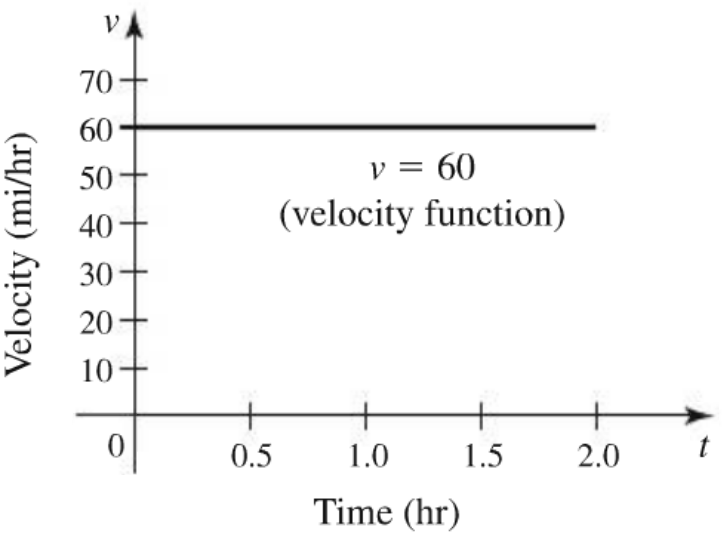
\includegraphics[width=0.35\linewidth]{images/briggs_05_01/velocityPlot_empty.png}
    \hspace*{\stretch{1}}
    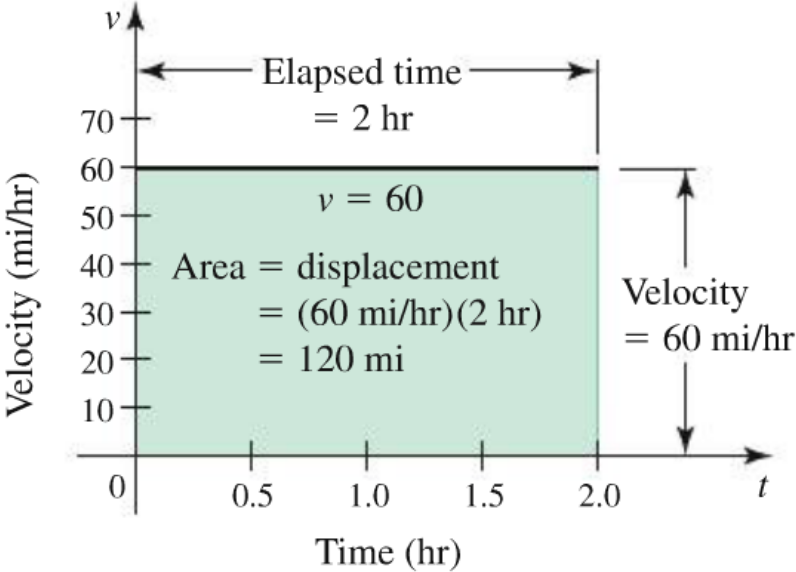
\includegraphics[width=0.35\linewidth]{images/briggs_05_01/velocityPlot_filled.png}
    \hspace*{\stretch{1}}
  \end{center}
\pagebreak

  For functions whose curves are irregular shapes, we can approximate the area using rectangles:
  \begin{center}
    \begin{tikzpicture}
      \begin{groupplot}[
        group style={group size=3 by 1, horizontal sep=0.25in},
        axis lines=center,
        xmin=-0.125, xmax=1.10,
        xtick={0,1},
        ymin=-0.125, ymax=1.25,
        width=0.375\linewidth,
        axis line style={->},
        ticklabel style={font=\footnotesize,inner sep=0.5pt,fill=white,opacity=1.0, text opacity=1},
        every axis plot/.append style={line width=0.75pt, color=blue, samples=100}
        ]
        \def\f(#1){1-(#1)^2};
        \def\a{0} \def\b{1}
        \def\n{4}            %% Number of rectangles
        %
        \FPsub\LEN\b\a       %% \LEN=\b-\a
        \FPdiv\del\LEN\n     %% \del=\LEN/\n
        \nextgroupplot
          \def\ALPHA{0.0}      %% left,center,right 0\leq \ALPHA\leq 1
          \FPmul\LR\del\ALPHA  %% \LR=\del*\ALPHA
          \pgfplotsinvokeforeach{\a,\a+\del,...,\b-\del}{
            \draw[left color=ClemsonPurple!75, right color=ClemsonPurple!40, line width=0.0pt] (axis cs: #1, 0) rectangle (#1+\del, {\f(\LR+#1)});}
          \addplot[name path=f, -] expression[domain=0:1]{\f(\x)};
        %
        %
        \nextgroupplot
        \def\ALPHA{0.5}      %% left,center,right 0\leq \ALPHA\leq 1
        \FPmul\LR\del\ALPHA  %% \LR=\del*\ALPHA
          \pgfplotsinvokeforeach{\a,\a+\del,...,\b-\del}{
            \draw[left color=ClemsonPurple!75, right color=ClemsonPurple!40, line width=0.0pt] (axis cs: #1, 0) rectangle (#1+\del, {\f(\LR+#1)});}
          \addplot[name path=f, -] expression[domain=0:1]{\f(\x)};
        %
        %
        \nextgroupplot
        \def\ALPHA{1.0}      %% left,center,right 0\leq \ALPHA\leq 1
        \FPmul\LR\del\ALPHA  %% \LR=\del*\ALPHA
          \pgfplotsinvokeforeach{\a,\a+\del,...,\b-\del}{
            \draw[left color=ClemsonPurple!75, right color=ClemsonPurple!40, line width=0.0pt] (axis cs: #1, 0) rectangle (#1+\del, {\f(\LR+#1)});}
          \addplot[name path=f, -] expression[domain=0:1]{\f(\x)};
      \end{groupplot}
    \end{tikzpicture}

    \begin{tabularx}{0.995\linewidth}{*{3}{Y}}
      Left rectangles&
      Midpoint rectangles&
      Right rectangles
    \end{tabularx}
  \end{center}
  \vspace*{\stretch{1}}
  
  These approximations are much more accurate when more rectangles are used:
  \begin{center}
    \begin{tikzpicture}
      \begin{groupplot}[
        group style={group size=3 by 1, horizontal sep=0.25in},
        axis lines=center,
        xmin=-0.125, xmax=1.15,
        ymin=-0.125, ymax=1.25,
        width=0.375\linewidth,
        axis line style={->},
        ticklabel style={font=\footnotesize,inner sep=0.5pt,fill=white,opacity=1.0, text opacity=1},
        every axis plot/.append style={line width=0.75pt, color=blue, samples=100}
        ]
        \def\f(#1){1-(#1)^2};
        \def\a{0} \def\b{1}
        \nextgroupplot[xtick={0,0.25,...,1},minor x tick num=1]
          \def\n{8}            %% Number of rectangles
          %
          \FPsub\LEN\b\a       %% \LEN=\b-\a
          \FPdiv\del\LEN\n     %% \del=\LEN/\n
          \def\ALPHA{0.0}      %% left,center,right 0\leq \ALPHA\leq 1
          \FPmul\LR\del\ALPHA  %% \LR=\del*\ALPHA
          \pgfplotsinvokeforeach{\a,\a+\del,...,\b-\del}{
            \draw[left color=ClemsonPurple!75, right color=ClemsonPurple!40, line width=0.0pt] (axis cs: #1, 0) rectangle (#1+\del, {\f(\LR+#1)});}
          \addplot[name path=f, -] expression[domain=0:1]{\f(\x)};
        %
        %
        \nextgroupplot[xtick={0,0.25,...,1},minor x tick num=3]
          \def\n{16}            %% Number of rectangles
          %
          \FPsub\LEN\b\a       %% \LEN=\b-\a
          \FPdiv\del\LEN\n     %% \del=\LEN/\n
          \def\ALPHA{0.0}      %% left,center,right 0\leq \ALPHA\leq 1
          \FPmul\LR\del\ALPHA  %% \LR=\del*\ALPHA
          \pgfplotsinvokeforeach{\a,\a+\del,...,\b-\del}{
            \draw[left color=ClemsonPurple!75, right color=ClemsonPurple!40, line width=0.0pt] (axis cs: #1, 0) rectangle (#1+\del, {\f(\LR+#1)});}
          \addplot[name path=f, -] expression[domain=0:1]{\f(\x)};
        %
        %
        \nextgroupplot[xtick={0,0.25,...,1},minor x tick num=7]
          \def\n{32}            %% Number of rectangles
          %
          \FPsub\LEN\b\a       %% \LEN=\b-\a
          \FPdiv\del\LEN\n     %% \del=\LEN/\n
          \def\ALPHA{0.0}      %% left,center,right 0\leq \ALPHA\leq 1
          \FPmul\LR\del\ALPHA  %% \LR=\del*\ALPHA
          \pgfplotsinvokeforeach{\a,\a+\del,...,\b-\del}{
            \draw[left color=ClemsonPurple!60, right color=ClemsonPurple!40, line width=0.0025pt] (axis cs: #1, 0) rectangle (#1+\del, {\f(\LR+#1)});}
          \addplot[name path=f, -] expression[domain=0:1]{\f(\x)};
      \end{groupplot}
    \end{tikzpicture}
  \end{center}
  \vspace*{\stretch{1}}
  \pagebreak
  
  \begin{defn*}[Riemann Sum]
    Suppose $f$ is defined on a closed interval $\sbrkt{a,b}$, which is divided into $n$ subintervals of equal length $\Delta x$. If $x_k^*$ is any point in the $k$-th subinterval $\sbrkt{x_{k-1},x_k}$, for $k=1,2,\dots,n$, then
      \[f(x_1^*)\Delta x+f(x_2^*)\Delta x+\dots+f(x_n^*)\Delta x\]
    is called a \textbf{Riemann sum} for $f$ on $\sbrkt{a,b}$. This sum is called
    \begin{itemize}
        \item 
          a \textbf{left Riemann sum} if $x_k^*$ is the left endpoint of $\sbrkt{x_{k-1},x_k}$,
        \item 
          a \textbf{right Riemann sum} if $x_k^*$ is the right endpoint of $\sbrkt{x_{k-1},x_k}$, and 
        \item 
          a \textbf{midpoint Riemann sum} if $x_k^*$ is the midpoint of $\sbrkt{x_{k-1},x_k}$, for $k=1,2,\dots, n$.
    \end{itemize}
    
    In general, midpoint rectangles give better approximations then left or right rectangles.
  \end{defn*}
  \vspace*{\stretch{1}}
  
  \begin{center}
    \begin{tabularx}{\linewidth}{*{3}{X}}
      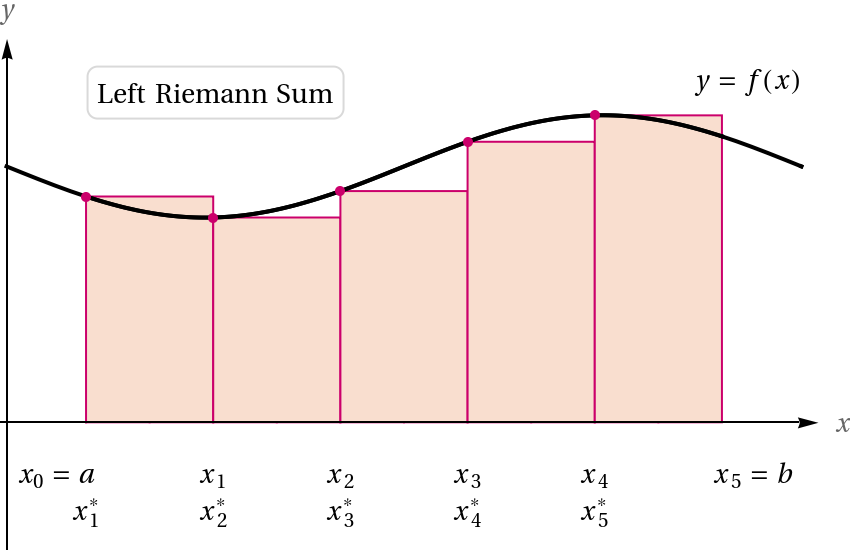
\includegraphics[width=\linewidth]{images/briggs_05_01/riemannSumLeft.png}&
      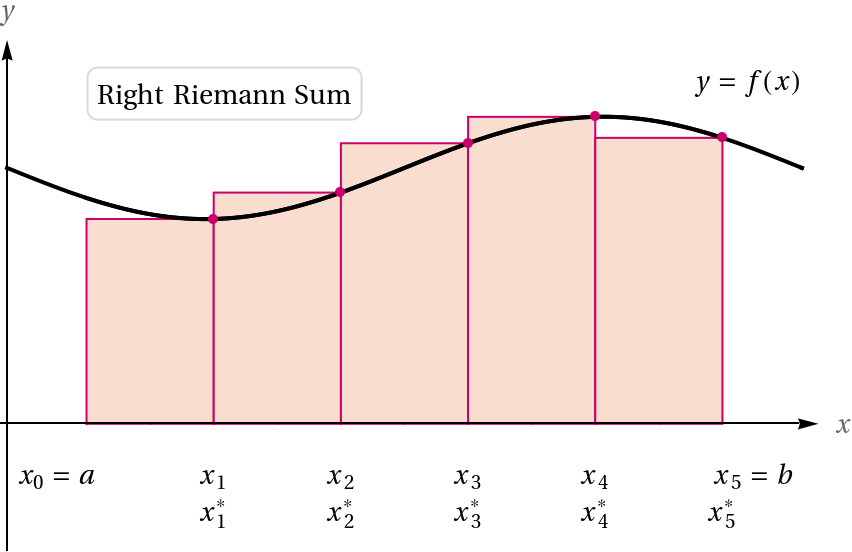
\includegraphics[width=\linewidth]{images/briggs_05_01/riemannSumRight.png}&
      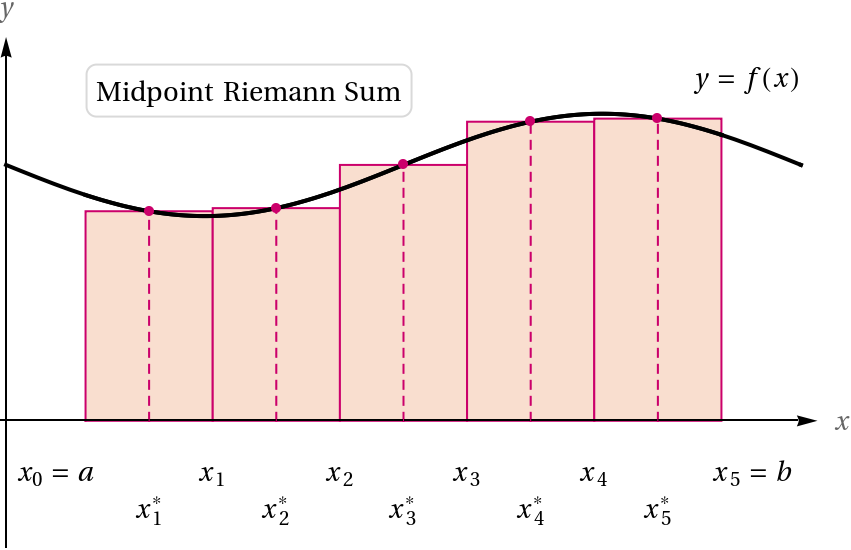
\includegraphics[width=\linewidth]{images/briggs_05_01/riemannSumMid.png}
    \end{tabularx}
  \end{center}
  \vspace*{\stretch{1}}
  \begin{quote}
    \noindent
    When estimating the area under the graph on the interval $\sbrkt{a,b}$, we define
      \[\Delta x=\dfrac{b-a}{n}\]
    to be the width of the rectangles. The height of the rectangles is given by $f(x_i)$, where the $x_i$'s are $\Delta x$ apart.
  \end{quote}
  \vspace*{\stretch{1}}
  \pagebreak
  
  \begin{ex*}
    Use the plots below to estimate the area under the given graph of $f(x)$:
  \end{ex*}
  \def\plotOne{
  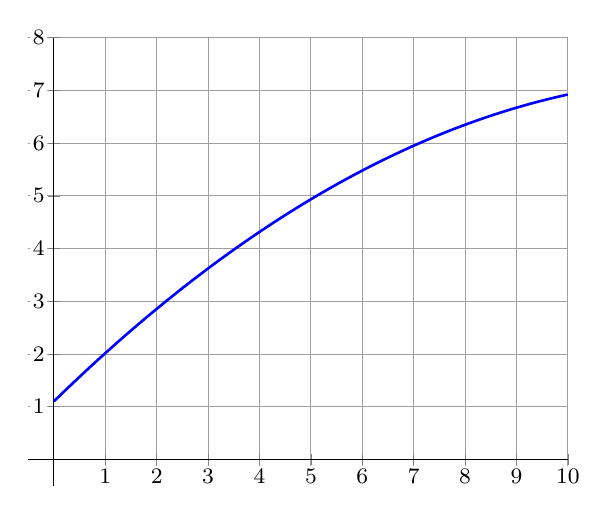
\begin{tikzpicture}
    \begin{axis}[
      grid=both,
      grid style={line width=0.35pt, draw=gray!75},
      axis lines=center,
      axis line style={-},
      xmin=-0.5, xmax=10,
      ymin=-0.5, ymax=8,
      xtick={0,1,...,10},
      ytick={0,1,...,8},
      ticklabel style={font=\footnotesize,inner sep=1pt,fill=white,opacity=1.0, text opacity=1},
      every axis plot/.append style={line width=0.95pt, color=blue, samples=100}
      ]
      \addplot[-] expression[domain=0:10] {-0.0369*x^2+0.95074*x+1.10261};
    \end{axis}
  \end{tikzpicture}
   }
  \begin{tasks}[after-item-skip=\stretch{1}, label=\mbox{}](1)
    \task 
      Sketch five rectangles and use them to find a lower estimate for the area under the given graph of $f(x)$ from $x=0$ to $x=10$.
      
      \begin{center}
        \plotOne
      \end{center}
    
    \task 
      Sketch five rectangles and use them to find a upper estimate for the area under the given graph of $f(x)$ from $x=0$ to $x=10$.
            
      \begin{center}
        \plotOne
      \end{center}
    
  \end{tasks}
  \vspace*{\stretch{1}}
  \pagebreak
  \def\plotTwo{
  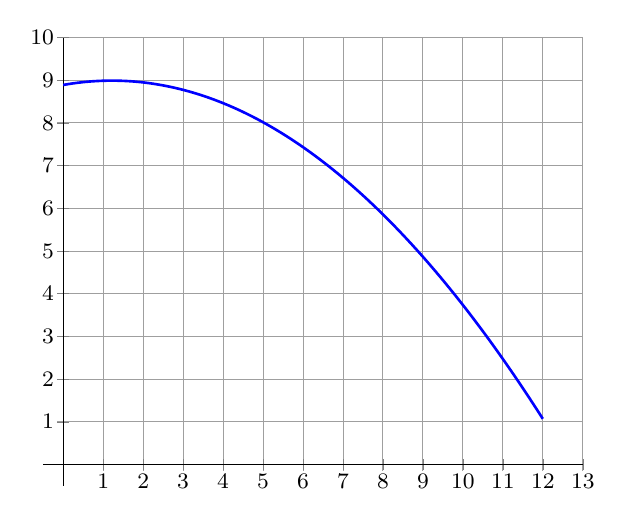
\begin{tikzpicture}
    \begin{axis}[
      grid=both,
      grid style={line width=0.35pt, draw=gray!75},
      axis lines=center,
      axis line style={-},
      xmin=-0.5, xmax=13,
      ymin=-0.5, ymax=10,
      xtick={0,1,...,13},
      ytick={0,1,...,10},
      ticklabel style={font=\footnotesize,inner sep=1pt,fill=white,opacity=1.0, text opacity=1},
      every axis plot/.append style={line width=0.95pt, color=blue, samples=100}
      ]
      \addplot[-] expression[domain=0:12] {-0.068154*x^2+0.16607*x+8.89047};
    \end{axis}
  \end{tikzpicture}
   }
  \begin{tasks}[after-item-skip=\stretch{1}, label=\mbox{}](1)
    \task 
      Use six right rectangles to estimate the area under the given graph of $f(x)$ from $x=0$ to $x=12$. Is the estimate an under-approximation or an over-approximation? Why?
      \begin{center}
        \plotTwo
      \end{center}
    
    \task 
      Use six midpoint rectangles to estimate the area under the given graph of $f(x)$ from $x=0$ to $x=12$. Talk about the quality of this estimate.
      \begin{center}
        \plotTwo
      \end{center}
  \end{tasks}
  \vspace*{\stretch{1}}
  \pagebreak
  
  \begin{ex*}
    Consider $f(x)=x^2$ on the interval $\sbrkt{0,1}$.
  \end{ex*}
  \newcommand{\blankAxis}{
    \begin{tikzpicture}[scale=0.775]
      \begin{axis}[
        axis lines=center,
        axis line style={-, line width=0.8pt},
        xmin=-0.125, xmax=1.25,
        ymin=-0.25, ymax=2,
        xtick={0.5,1},
        xticklabels={$\sfrac{1}{2}$,$1$},
        ymajorticks=false,
        minor x tick num=1,
        ticklabel style={font=\normalsize,inner sep=0.5pt,fill=white,opacity=1.0, text opacity=1},
        every axis plot/.append style={line width=0.95pt, color=blue, samples=100}
        ]
      \end{axis}
    \end{tikzpicture}
  }
  \begin{tasks}[after-item-skip=\stretch{1}](1)
    \task 
      Use two rectangles of equal width to find a lower sum for the area under the graph of $f(x)$.
      
      \blankAxis
    \task 
      Use four rectangles of equal width to find an upper sum for the area under the graph of $f(x)$.
      
      
      \blankAxis
    \task 
      Use four midpoint rectangles of equal width to estimate the area under the graph of $f(x)$.
      
      \blankAxis
  \end{tasks}
  \vspace*{\stretch{1}}
  \pagebreak
  
  \renewcommand{\blankAxis}{
    \begin{tikzpicture}[scale=0.775]
      \begin{axis}[
        axis lines=center,
        axis line style={-, line width=0.8pt},
        xmin=-0.525, xmax=5.25,
        ymin=-0.25, ymax=2,
        xtick={1,2,...,5},
        xticklabels={,$2$,,$4$,},
        ymajorticks=false,
        minor x tick num=0,
        ticklabel style={font=\normalsize,inner sep=0.5pt,fill=white,opacity=1.0, text opacity=1},
        every axis plot/.append style={line width=0.95pt, color=blue, samples=100}
        ]
      \end{axis}
    \end{tikzpicture}
  }
  \begin{ex*}
    Consider $f(x)=\dfrac{1}{x}$ on the interval $\sbrkt{1,5}$.
  \end{ex*}

  \vspace*{-10pt}

  \begin{tasks}[after-item-skip=\stretch{1}](1)
    \task 
      Use two rectangles of equal width to find a lower sum for the area under the graph of $f(x)$.
      
      \blankAxis
    \task 
      Use four rectangles of equal width to find a lower sum for the area under the graph of $f(x)$.
      
      \blankAxis
    \task 
      Use two rectangles of equal width to find an upper sum for the area under the graph of $f(x)$.
      
      \blankAxis
  \end{tasks}
  \vspace*{\stretch{1}}
  \pagebreak
  
  \begin{tasks}[after-item-skip=\stretch{1}, resume](1)
    \task 
      Use four rectangles of equal width to find an upper sum for the area under the graph of $f(x)$.
      
      \blankAxis
    \task 
      Use two midpoint rectangles of equal width to estimate the area under the graph of $f(x)$.
      
      \blankAxis
    \task 
      Use four midpoint rectangles of equal width to estimate the area under the graph of $f(x)$.
      
      \begin{tikzpicture}[scale=0.775]
        \begin{axis}[
          axis lines=center,
          axis line style={-, line width=0.8pt},
          xmin=-0.525, xmax=5.25,
          ymin=-0.25, ymax=2,
          xtick={1,2,...,5},
          xticklabels={,$2$,,$4$,},
          ymajorticks=false,
          minor x tick num=1,
          ticklabel style={font=\normalsize,inner sep=0.5pt,fill=white,opacity=1.0, text opacity=1},
          every axis plot/.append style={line width=0.95pt, color=blue, samples=100}
          ]
        \end{axis}
      \end{tikzpicture}
  \end{tasks}
  \vspace*{\stretch{1}}
  \pagebreak
  
  \begin{ex*}
    Use the tabulated values of $f$ to evaluate both the left and right Riemann sums. ($n=8$, $\sbrkt{1,5}$)
  \end{ex*}
  \begin{center}
    \begin{tabular}{@{}L*{9}{|>{\raggedleft\arraybackslash}p{0.35in}}@{}}
      x& 1& 1.5& 2& 2.5& 3& 3.5& 4& 4.5& 5\\\hline
      f(x)& 0& 2& 3& 2& 2& 1& 0& 2& 3
    \end{tabular}
  \end{center}
  \vspace*{\stretch{1}}
  
  \noindent
  When velocity is a continuous function, the area between the curve and the $x$-axis gives the displacement.
  \begin{ex*}
    The velocities (in $m/s$) of an automobile moving along a straight freeway over a four-second period are given in the following table. Find the midpoint Riemann sum approximation to the displacement on $\sbrkt{0,4}$ with $n=2$ and $n=4$ subintervals.
  \end{ex*}
  \begin{center}
    \begin{tabular}{@{}L*{9}{|>{\raggedleft\arraybackslash}p{0.35in}}@{}}
      t   &  0& 0.5&  1& 1.5&  2& 2.5&  3& 3.5& 4\\\hline
      v(t)& 20&  25& 30&  35& 30&  30& 35&  40& 40
    \end{tabular}
  \end{center}
  \vspace*{\stretch{1}}
  \pagebreak
  
  \begin{ex*}
    Use the following table of recorded velocities answer the following questions:
  \end{ex*}
  \begin{center}
    \begin{tabular}{@{}*{2}{p{0.775in}}|*{2}{>{\raggedleft\arraybackslash}p{0.775in}}@{}}\hline
      \lnret[l]{\textbf{Time}\\\textbf{(min)}}& 
      \lnret[l]{\textbf{Velocity}\\\textbf{(m/sec)}}& 
      \lnret[l]{\textbf{Time}\\\textbf{(min)}}& 
      \lnret[l]{\textbf{Velocity}\\\textbf{(m/sec)}}\\\hline
      %
       0& 1.0& 35& 1.2\\
       5& 1.2& 40& 1.0\\
      10& 1.7& 45& 1.8\\
      15& 2.0& 50& 1.5\\
      20& 1.8& 55& 1.2\\
      25& 1.6& 60& 0\\
      30& 1.4&\\\hline
    \end{tabular}
  \end{center}
  \begin{tasks}[after-item-skip=\stretch{1}](1)
    \task 
      Estimate the total displacement using 12 subintervals of length 5 with left-endpoint values.
    \task 
      Estimate the total displacement using 12 subintervals of length 5 with right-endpoint values.
  \end{tasks}
  \vspace*{\stretch{1}}
  \pagebreak
  
  \begin{defn*}
    If $a_m, a_{m+1},\dots,a_n$ are real numbers and $m$ and $n$ are integers such that $m\leq n$, then
      \[\sum\ito[m]^n a_i=a_m+a_{m+1}+\cdots+a_\nmo+a_n\]
  \end{defn*}
  \begin{ex*}
    Rewrite the sums without sigma notation and evaluate:
  \end{ex*}
  \begin{tasks}(2)
    \task $\ds\sum\kto^3 \frac{k-1}{k}$
    \task $\ds\sum\kto^4 \parens{-1}^k \cos(k\pi)$
  \end{tasks}
  \vspace*{\stretch{1}}
  \begin{ex*}
    Rewrite the following sum without sigma notation. Note that $n$ denotes the number of rectangles and the letters $i$, $j$, and $k$ are typically used for indexing.
      \[\sum\kto^n \frac{1}{n}(k^2+1)\]
  \end{ex*}
  \vspace*{\stretch{1}}
  \pagebreak
  
  \begin{ex*}
    Which of the following summations represent the sum $1+2+4+8+16+32$?
    \begin{tasks}(3)
      \task $\ds\sum\kto^6 2^{k-1}$
      \task $\ds\sum\kto[0]^5 2^k$
      \task $\ds\sum\kto[-1]^4 2^{k+1}$
    \end{tasks}
  \end{ex*}
  \vspace*{\stretch{1}}
  
  \begin{ex*}
    Which of the following summations represent the sum $1-2+4-8+16-32$?
    \begin{tasks}(3)
      \task $\ds\sum\kto^6 (-2)^{k-1}$
      \task $\ds\sum\kto[0]^5 (-1)^k2^k$
      \task $\ds\sum\kto[-2]^3 (-1)^{k+1}2^{k+2}$
    \end{tasks}
  \end{ex*}
  \vspace*{\stretch{1}}
  \pagebreak
  
  \begin{ex*}
    Express the following sums in sigma notation:
  \end{ex*}
  \begin{tasks}[after-item-skip=\stretch{1}](2)
    \task $-1+4-9+16-25$
    \task $\dfrac{1}{2}+\dfrac{1}{4}+\dfrac{1}{8}+\dfrac{1}{16}$
    \task $\dfrac{5}{2}+\dfrac{10}{3}+\dfrac{15}{4}+\dfrac{20}{5}+\dfrac{25}{6}+\dfrac{30}{7}$
    \task $4+9+14+\cdots+44$
  \end{tasks}
  \vspace*{\stretch{1}}
  
  \begin{ex*}
    Suppose that $\Sum\kto^n a_k=0$ and $\Sum\kto^n b_k=1$, evaluate the following
  \end{ex*}
  \begin{tasks}[after-item-skip=\stretch{1}](2)
    \task $\ds\sum\kto^n 8a_k$
    \task $\ds\sum\kto^n 250b_k$
    \task $\ds\sum\kto^n (a_k+1)$
    \task $\ds\sum\kto^n (b_k-1)$
  \end{tasks}
  \vspace*{\stretch{1}}
  \pagebreak
  
  \noindent
  \fbox{\parbox{0.9875\linewidth}{
    \textbf{Theorem 5.1: Sums of Powers of Integers}
    
    Let $n$ be a positive integer and $c$ a real number.
    \begin{align*}
      \sum\kto^n c&=cn& 
      \sum\kto^n k &=\frac{n(n+1)}{2}\\
      \sum\kto^n k^2&=\frac{n(n+1)(2n+1)}{6}&
      \sum\kto^n k^3&=\frac{n^2(n+1)^2}{4}
    \end{align*}
  }}
  
  \begin{ex*}
    Prove that $\ds\sum\kto^n k=\frac{n(n+1)}{2}$
  \end{ex*}
  \vspace*{\stretch{1}}
  \begin{ex*}
    Evaluate the following sums
  \end{ex*}
  \begin{tasks}[after-item-skip=\stretch{0.5}](3)
    \task $\ds\sum\kto^{10} k$
    \task $\ds\sum\kto^{10} \parens{1+k^2}$
    \task $\ds\sum\kto^{10} k^3$
    \task $\ds\sum\kto^7 (-2k-4)$
    \task $\ds\sum\kto^6 (3-k^2)$
    \task $\ds\sum_{m=1}^3 \frac{2m+2}{3}$
  \end{tasks}
  \vspace*{\stretch{0.5}}
  \pagebreak
  
  \begin{defn*}[Left, Right and Midpoint Riemann Sums in Sigma Notation]
    Suppose $f$ is defined on a closed interval $\sbrkt{a,b}$, which is divided into $n$ subintervals of equal length $\Delta x$. If $x_k^*$ is a point in the $k$th subinterval $\sbrkt{x_{k-1},x_k}$, for $k=1,2,\dots, n$, then the \textbf{Riemann sum} for $f$ on $\sbrkt{a,b}$ is $\ds\sum\kto^n f\parens{x_k^*}\Delta x$. Three cases arise in practice.
    \begin{itemize}
      \item 
        $\ds\sum\kto^n f(x_k^*)\Delta x$ is a \textbf{left Riemann sum} if $x_k^*=a+(k-1)\Delta x$.
      \item 
        $\ds\sum\kto^n f(x_k^*)\Delta x$ is a \textbf{right Riemann sum} if $x_k^*=a+k\Delta x$.
      \item 
        $\ds\sum\kto^n f(x_k^*)\Delta x$ is a \textbf{midpoint Riemann sum} if $x_k^*=a+(k-\sfrac{1}{2})\Delta x$.
    \end{itemize}
  \end{defn*}
  \begin{ex*}
    For the function $f(x)=3x^2$, find a formula for the upper sum obtained by dividing the interval $\sbrkt{0,1}$ into $n$ equal subintervals.
  \end{ex*}
  \vspace*{\stretch{1}}
  \noindent
  Now take the limit of the sum as $n\to\infty$ to calculate the area under $f(x)=3x^2$ over $\sbrkt{0,1}$.
  \vspace*{\stretch{0.5}}
  \pagebreak
  
  \begin{ex*}
    For the function $f(x)=2x$, find a formula for the upper sum obtained by dividing the interval $\sbrkt{0,3}$ into $n$ equal subintervals.
  \end{ex*}
  \vspace*{\stretch{1}}
  \noindent
  Now take the limit of the sum as $n\to\infty$ to calculate the area under $f(x)=2x$ over $\sbrkt{0,3}$.
  \vspace*{\stretch{1}}
  \pagebreak
  
\end{document}

\documentclass[answers]{exam}
\usepackage{texPreamble}
\usepackage{relsize}
\usepackage{tabularx}
\extraheadheight{0.25in}
\extrafootheight{1.0in}
\extrawidth{1in}
% ----------------------------------------------------------------
\firstpagefootrule
\runningfootrule
\begin{document}
%\relscale{1.4}
\section{5.2: Definite Integrals}
In section 5.1, we assumed $f$ was nonnegative on the interval $\sbrkt{a,b}$. 

\noindent
When $f(x)\leq 0$ on the interval $\sbrkt{a,b}$, then the area between $f(x)$ and the $x$-axis is negative.
\vspace*{\stretch{1}}
\begin{ex*}
  Consider the function $x^3-1$ on $\sbrkt{-2,0}$. Using Riemann sums, we can approximate the area between the curve and the $x$-axis:
\end{ex*}
\vspace*{15pt}

\def\a{-2}           %% START
\def\b{0}            %% STOP
\def\n{4}            %% Number of rectangles
%
\FPsub\LEN\b\a       %% \LEN=\b-\a
\FPdiv\del\LEN\n     %% \del=\LEN/\n
\def\f(#1){(#1)^3-1}
\hspace*{\stretch{1}}
\begin{tikzpicture}[scale=0.825]
  \begin{groupplot}[
    group style={group size=3 by 1, horizontal sep=0.5cm},
    axis lines=center,
    axis line style={->},
    xmin=-2.5, xmax=2.5,
    ticklabel style={font=\footnotesize,inner sep=0.5pt,fill=white,opacity=1.0, text opacity=1},
    every axis plot/.append style={line width=0.95pt, color=blue, samples=100}
    ]
    \nextgroupplot 
      \def\ALPHA{0.0}      %% left,center,right 0\leq \ALPHA\leq 1
      \FPmul\LR\del\ALPHA  %% \LR=\del*\ALPHA
      \pgfplotsinvokeforeach{\a,\a+\del,...,\b-\del}{
        \draw[left color=red!95, right color=red!40, line width=0.0pt] 
        (axis cs: #1, 0) rectangle (#1+\del, {\f(\LR+#1)});}
      \addplot[-] expression[domain=-2.015:1.75]{\f(x)};
    \nextgroupplot 
      \def\ALPHA{0.5}      %% left,center,right 0\leq \ALPHA\leq 1
      \FPmul\LR\del\ALPHA  %% \LR=\del*\ALPHA
      \pgfplotsinvokeforeach{\a,\a+\del,...,\b-\del}{
        \draw[left color=red!95, right color=red!40, line width=0.0pt] 
        (axis cs: #1, 0) rectangle (#1+\del, {\f(\LR+#1)});}
      \addplot[-] expression[domain=-2.015:1.75]{\f(x)};
    \nextgroupplot 
      \def\ALPHA{1.0}      %% left,center,right 0\leq \ALPHA\leq 1
      \FPmul\LR\del\ALPHA  %% \LR=\del*\ALPHA
      \pgfplotsinvokeforeach{\a,\a+\del,...,\b-\del}{
        \draw[left color=red!95, right color=red!40, line width=0.0pt] 
        (axis cs: #1, 0) rectangle (#1+\del, {\f(\LR+#1)});}
      \addplot[-] expression[domain=-2.015:1.75]{\f(x)};
  \end{groupplot}
\end{tikzpicture}
\hspace*{\stretch{1}}
\begin{center}
  \parbox{0.8\linewidth}{
  \begin{align*}
    L_4&= f(-2)\frac{1}{2}+f(-1.5)\frac{1}{2}+f(-1)\frac{1}{2}+f(-0.5)\frac{1}{2}&
      &=-8.25\\[\baselineskip]
    M_4&= f(-1.75)\frac{1}{2}+f(-1.25)\frac{1}{2}+f(-0.75)\frac{1}{2}+f(-0.25)\frac{1}{2}&
      &=-5.875\\[\baselineskip]
    R_4&= f(-1.5)\frac{1}{2}+f(-1)\frac{1}{2}+f(-0.5)\frac{1}{2}+f(0)\frac{1}{2}&
      &=-4.25
  \end{align*}}
\end{center}
Actual area: $\boxed{-6}$
\vspace*{\stretch{1}}
\pagebreak
\begin{defn*}[Net Area]
  Consider the region $R$ bounded by the graph of a continuous function $f$ and the $x$-axis between $x=a$ and $x=b$. The \textbf{net area} of $R$ is the sum of the areas of the parts of $R$ that lie above the $x$-axis \textit{minus} the sum of the areas of the parts of $R$ that lie below the $x$-axis on $\sbrkt{a,b}$.
\end{defn*}
\begin{ex*}
  If $f(x)=x^2-2x,\ 0\leq x\leq 3$, evaluate the Riemann sum with $n=6$, taking the sample points to be right endpoints. 

\vspace*{\stretch{1}}
  \begin{tikzpicture}
    \begin{axis}[
      %grid=both,
      %grid style={line width=0.35pt, draw=gray!75},
      axis lines=center,
      axis line style={-},
      xmin=-0.5, xmax=4,
      ymin=-1, ymax=4,
      xtick={0,1,...,3},
      ymajorticks=false,
      ticklabel style={font=\footnotesize,inner sep=1pt,fill=white,opacity=1.0, text opacity=1},
      every axis plot/.append style={line width=0.95pt, color=blue, samples=100}
      ]
    \end{axis}
  \end{tikzpicture}
\end{ex*}

\begin{ex*}
  Find the Riemann sum for $f(x)=\sin(x),\ 0\leq x\leq \frac{3\pi}{2}$, with six terms, taking the sample points to be right endpoints.

\vspace*{\stretch{1}}
  \begin{tikzpicture}
    \begin{axis}[
      %grid=both,
      %grid style={line width=0.35pt, draw=gray!75},
      axis lines=center,
      axis line style={-},
      xmin=-0.6, xmax=4.75,
      ymin=-1, ymax=1,
      xtick={0,1.570796327,...,5},
      xticklabels = {,$\frac{\pi}{2}$, $\pi$, $\frac{3\pi}{2}$},
      ymajorticks=false,
      minor x tick num = 1,
      ticklabel style={font=\footnotesize,inner sep=1pt,fill=white,opacity=1.0, text opacity=1},
      every axis plot/.append style={line width=0.95pt, color=blue, samples=100}
      ]
    \end{axis}
  \end{tikzpicture}
\end{ex*}
\pagebreak

\begin{defn*}[Definite Integral]
  A function $f$ defined on $\sbrkt{a,b}$ is \textbf{integrable} on $\sbrkt{a,b}$ if $\ds\lim_{n\to \infty} \sum\kto^n f(x_k^*)\Delta x_k$ exists and is unique over all partitions of $\sbrkt{a,b}$ and all choices of $x_k^*$ on a partition. This limit is the \textbf{definite integral of $f$ from $a$ to $b$}, which we write
  \[\int_a^b f(x)\,dx=\lim_{n\to \infty}\sum\kto^n f(x_k^*)\Delta x_k\]
\end{defn*}

\begin{center}
  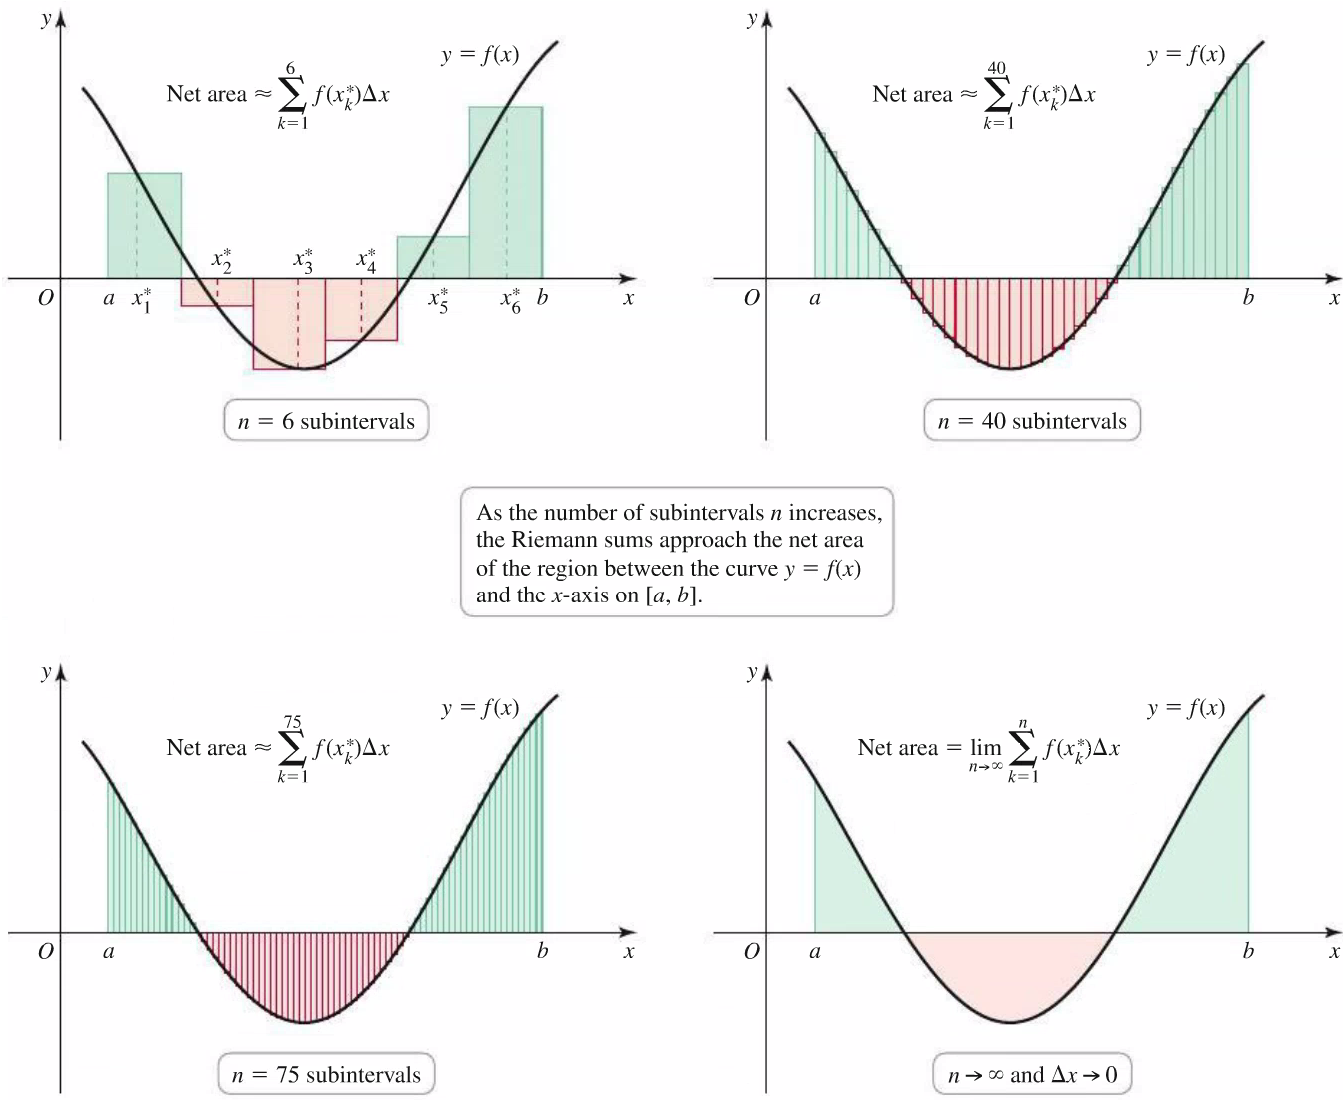
\includegraphics[width=0.85\linewidth]{images/briggs_05_02/fig5_20.png}
\end{center}
\pagebreak
\begin{ex*}~

  \begin{tasks}[after-item-skip=\stretch{1}](1)
    \task 
      For the function $f(x)=3x+2x^2$, find a formula for the upper sum obtained by dividing the interval $\sbrkt{0,1}$ into $n$ equal subintervals.
    \task 
      Take the limit of the sum as $n\to\infty$ to calculate the area under $f(x)=3x+2x^2$ over $\sbrkt{0,1}$.
  \end{tasks}
\end{ex*}
\vspace*{\stretch{0.25}}
\pagebreak

\begin{ex*}
  Use the limit of the Riemann sum notation to evaluate $\ds\int_0^2 (2-x^2)\,dx$.
\end{ex*}
\vspace*{\stretch{1}}
\begin{ex*}
  Use the definition of the definite integral to evaluate $\ds\int_1^4 \parens{x^2-1}\,dx$.
\end{ex*}
\vspace*{\stretch{1}}
\pagebreak

\begin{ex*}
  Use the definition of the definite integral to evaluate $\ds\int_1^4 \parens{x^2-4x+2}\,dx$.
\end{ex*}
\vspace*{\stretch{1}}

\begin{ex*}
  Use the definition of the definite integral to evaluate $\ds\int_0^2 4x^3\,dx$.
\end{ex*}
\vspace*{\stretch{1}}
\pagebreak

\begin{ex*}
  Use a sketch and geometry to evaluate the following integral
  
  $\ds\int_1^{10} g(x)\,dx$, where $g(x)=
  \begin{cases}
    4x,& \textnormal{if } 0\leq x\leq 2\\
    -8x+16,& \textnormal{if } 2< x\leq 3\\
    -8,& \textnormal{if } x>3
  \end{cases}$
\end{ex*}
\begin{tikzpicture}
  \begin{axis}[
    axis lines=center,
    axis line style={-},
    xmin=-0.25, xmax=5,
    ymin=-8.5, ymax=8.5,
    xtick={1,2,...,4},
    ytick={-8,8},
    xticklabels = {,,,},
    width=0.5\linewidth,
    height=2.25in,
    ticklabel style={font=\footnotesize,inner sep=0.5pt,fill=white,opacity=1.0, text opacity=1},
    every axis plot/.append style={line width=0.95pt, color=blue, samples=100}
    ]
  \end{axis}
\end{tikzpicture}

\begin{ex*}
  Use the following figure to evaluate the integrals below:
  \begin{center}
    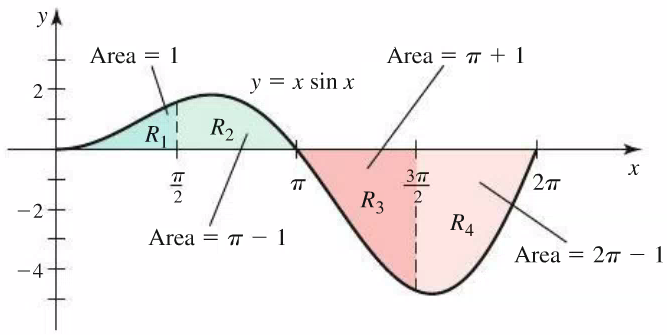
\includegraphics[width=0.4\linewidth]{images/briggs_05_02/q47_50.png}
  \end{center}
\end{ex*}

\begin{tasks}[after-item-skip=\stretch{1}](2)
  \task $\ds\int_{0}^{\pi} x\sin(x)\,dx$
  \task $\ds\int_{0}^{\sfrac{3\pi}{2}} x\sin(x)\,dx$
  \task $\ds\int_{0}^{2\pi} x\sin(x)\,dx$
  \task $\ds\int_{\sfrac{\pi}{2}}^{2\pi} x\sin(x)\,dx$
\end{tasks}
\vspace*{\stretch{1}}
\pagebreak

\begin{ex*}
  Graph the following integrands and compute the areas to evaluate the integrals.
\end{ex*}
\begin{tasks}[after-item-skip=\stretch{1}](2)
  \task $\ds\int_{\sfrac{1}{2}}^{\sfrac{3}{2}} \parens{-2x+4}\,dx$
  \task $\ds\int_{-2}^{4} \parens{\frac{x}{2}+3}\,dx$
  \task $\ds\int_{0}^{3} \parens{\frac{1}{2}x-1}\,dx$
  \task $\ds\int_{-1}^{3} \parens{3-2x}\,dx$
  \task $\ds\int_{-4}^{0} \sqrt{16-x^2}\,dx$
  \task $\ds\int_{-1}^{1} \parens{1+\sqrt{1-x^2}}\,dx$
  \task $\ds\int_{-2}^{1} \abs{x}\,dx$
  \task $\ds\int_{-1}^{1} \parens{2-\abs{x}}\,dx$
\end{tasks}
\vspace*{\stretch{1}}

\pagebreak

\fbox{\parbox{0.9875\linewidth}{
  \textbf{Properties of definite integrals}
  
  \parbox{0.95\linewidth}{\mbox{}%
  
  Let $f$ and $g$ be integrable functions on an interval that contains $a$, $b$, and $p$.
  
  \begin{enumerate}
    \item $\ds\int_a^a f(x)\,dx=0$
    \item $\ds\int_a^b f(x)\,dx=-\int_b^a f(x)\,dx$
    \item $\ds\int_a^b \parens{f(x)\pm g(x)}\,dx=\int_a^b f(x)\,dx\pm \int_a^b g(x)\,dx$
    \item $\ds\int_a^b c\,\!f(x)\,dx=c\!\int_a^b f(x)\,dx$, for any constant $c$
    \item $\ds\int_a^b f(x)\,dx=\int_a^p f(x)\,dx+\int_p^b f(x)\,dx$
    \item The function $\abs{f}$ is integrable on $\sbrkt{a,b}$ and $\int_a^b\abs{f(x)}\,dx$ is the sum of the areas of the regions bounded by the graph of $f$ and the $x$-axis on $\sbrkt{a,b}$.
  \end{enumerate}}
}}

\begin{center}
  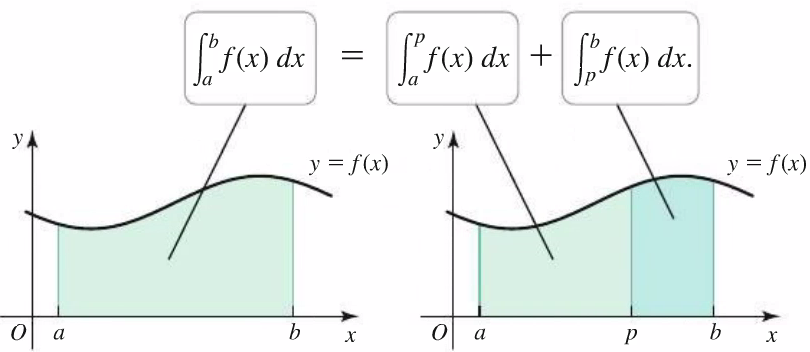
\includegraphics[width=0.5\linewidth]{images/briggs_05_02/fig5_29.png}\\[0.65\baselineskip]
  
  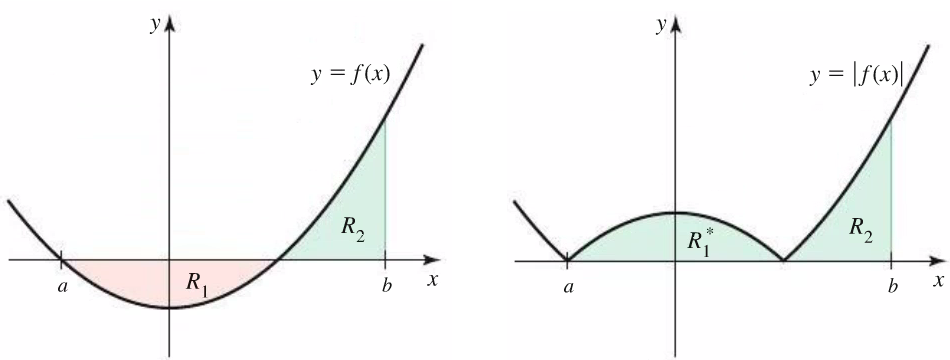
\includegraphics[width=0.5\linewidth]{images/briggs_05_02/fig5_31.png}
\end{center}
\pagebreak
\begin{ex*}
  Suppose that $\ds\int_{-3}^{0} g(t)\,dt=\sqrt 2$. Evaluate the following:
\end{ex*}
\begin{tasks}[after-item-skip=\stretch{1}](2)
  \task $\ds\int_{-3}^{0} g(u)\,du$
  \task $\ds\int_{0}^{-3} g(t)\,dt$
  \task $\ds\int_{0}^{-3} \sbrkt{-g(x)}\,dx$
  \task $\ds\int_{-3}^{0} \frac{g(r)}{\sqrt 2}\,dr$
\end{tasks}
\vspace*{\stretch{1}}

\begin{ex*}
  Suppose that $\ds\int_0^3 f(z)\,dz=3$ and $\ds\int_0^4 f(z)\,dz=7$. Evaluate the following:
\end{ex*}
\begin{tasks}(2)
  \task $\ds\int_3^4 f(z)\,dz$
  \task $\ds\int_4^3 f(z)\,dz$
\end{tasks}
\vspace*{\stretch{1}}
\pagebreak

\begin{ex*}
  Use the fact that $\ds\int_0^{\sfrac{\pi}{2}} \parens{\cos(\theta)-2\sin(\theta)}\,d\theta=-1$ to evaluate the following
\end{ex*}
\begin{tasks}(2)  
  \task $\ds\int_0^{\sfrac{\pi}{2}} \parens{2\sin(\theta)-\cos(\theta)}\,d\theta$
  \task $\ds\int_{\sfrac{\pi}{2}}^0 \parens{4\cos(\theta)-8\sin(\theta)}\,d\theta$
\end{tasks}
\vspace*{\stretch{1}}

\begin{ex*}
  Suppose that $\ds\int_1^9 f(x)\,dx=-1$, $\ds\int_7^9 f(x)\,dx=5$ and $\ds\int_7^9 h(x)\,dx=4$. Evaluate the following:
\end{ex*}
\begin{tasks}[after-item-skip=\stretch{1}](2)
  \task $\ds\int_1^9 -2f(x)\,dx$
  \task $\ds\int_7^9 \sbrkt{f(x)+h(x)}\,dx$
  \task $\ds\int_7^9 \sbrkt{2f(x)-3h(x)}\,dx$
  \task $\ds\int_9^1 f(x)\,dx$
  \task $\ds\int_1^7 f(x)\,dx$
  \task $\ds\int_7^9 \sbrkt{h(x)-f(x)}\,dx$
\end{tasks}
\vspace*{\stretch{1}}
\pagebreak
\begin{ex*}
  Given $\ds\int_1^3 e^x\,dx=e^3-e$, find $\ds\int_1^3 \parens{2e^x-1}\,dx$
\end{ex*}
\vspace*{\stretch{1}}

\begin{ex*}
  Suppose that $f(x)\geq 0$ on $\sbrkt{0,2}$ and $f(x)\leq 0$ on $\sbrkt{2,5}$ where $\ds\int_0^2 f(x)\,dx=6$ and $\ds\int_2^5 f(x)\,dx=-8$. Evaluate the following:
\end{ex*}
\begin{tasks}[after-item-skip=\stretch{1}](2)
  \task $\ds\int_0^5 f(x)\,dx$
  \task $\ds\int_0^5 \abs{f(x)}\,dx$
  \task $\ds\int_2^5 4\abs{f(x)}\,dx$
  \task $\ds\int_0^5 \parens{f(x)+\abs{f(x)}}\,dx$
\end{tasks}
\vspace*{\stretch{1}}
\pagebreak

\end{document}

\documentclass[answers]{exam}
\usepackage{texPreamble}
\usepackage{relsize}
\usepackage{tabularx}
\extraheadheight{0.25in}
\extrafootheight{1.0in}
\extrawidth{1in}
% ----------------------------------------------------------------
\firstpagefootrule
\runningfootrule
\begin{document}
%\relscale{1.4}
\section{5.3: Fundamental Theorem of Calculus}
\begin{defn*}[Area Function]
  Let $f$ be a continuous function, for $t\geq a$. The \textbf{area function for $f$ with left endpoint $a$ is}
    \[A(x)=\int_a^x f(t)\,dt\]
  where $x\geq a$. The area function gives the net area of the region bounded by the graph of $f$ and the $t$-axis on the interval $\sbrkt{a,x}$.
\end{defn*}
\begin{ex*}
  The graph of $f$ is shown in the figure. Let $A(x)=\int_0^x f(t)\,dt$ and $F(x)=\int_2^x f(t)\,dt$ be two area functions for $f$. Evaluate the following area functions:
\end{ex*}

  \hfill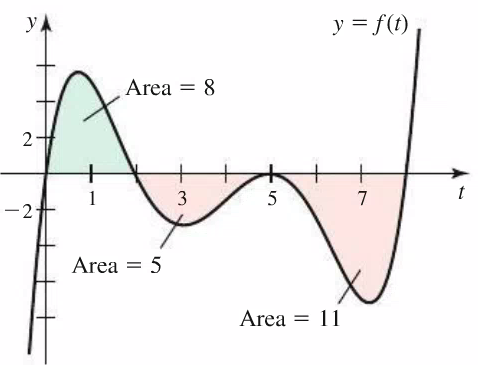
\includegraphics[width=0.5\linewidth]{images/briggs_05_03/q14.png}\hfill\mbox{} 

\begin{tasks}[after-item-skip=\stretch{1}](4)
  \task $A(2)$
  \task $F(5)$
  \task $A(0)$
  \task $F(8)$
  \task $A(8)$
  \task $A(5)$
  \task $F(2)$
\end{tasks}
\vspace*{\stretch{1}}
\pagebreak

\begin{ex*}
  Let $g(x)=\int_0^x f(t)\,dt$, where $f$ is the function whose graph is shown.
\end{ex*}
\noindent
\begin{minipage}[t]{0.55\linewidth}
  \begin{tasks}[after-item-skip=35pt](1)
    \task Evaluate $g(x)$ for $x=0,1,2,3,4,5$ and $6$.
    \task Estimate $g(7)$.
    \task Where does $g$ have a maximum value? Where does it have a minimum value?
  \end{tasks}
\end{minipage}
\begin{minipage}[t]{0.45\linewidth}\mbox{}
  \vspace*{-0.25\baselineskip}
  \begin{flushright}
    \begin{tikzpicture}
      \begin{axis}[
        grid=both,
        grid style={line width=0.35pt, draw=gray!75},
        axis lines=center,
        axis line style={-},
        xmin=-1, xmax=7.5,
        ymin=-2, ymax=4,
        xtick={-6,-5,...,7},
        ytick={-6,-5,...,6},
        ticklabel style={font=\footnotesize,inner sep=1.5pt,fill=white,opacity=1.0, text opacity=1},
        every axis plot/.append style={line width=0.95pt, color=blue, samples=100}
        ]
        \addplot[-] expression[domain=0:2]{1-x};
        \addplot[-] expression[domain=2:6]{x-3};
        \addplot[-] expression[domain=6:7]{-3*x^2+36*x-105};
      \end{axis}
    \end{tikzpicture}
    \hspace*{0pt}
  \end{flushright}
\end{minipage}
\vspace*{\stretch{1}}
\begin{ex*}
  For the area function $A(x)=\int_a^x f(t)\,dt$, graph the area function and then verify that $A'(x)=f(x)$.
\end{ex*}
\begin{tasks}[after-item-skip=\stretch{1}](1)
  \task $f(t)=10,\ a=4$
  \task $f(t)=2,\ a=-3$
\end{tasks}
\vspace*{\stretch{1}}
\pagebreak

\begin{tasks}[after-item-skip=\stretch{1}, resume](1)
  \task $f(t)=2t+5,\ a=0$
  \task $f(t)=4t+2,\ a=0$
\end{tasks}
\vspace*{\stretch{1}}

\begin{ex*}
  Let $f(x)=c$, where $c$ is a positive constant. Explain why an area function of $f$ is an increasing function.
\end{ex*}
\vspace*{\stretch{1}}

\begin{ex*}
  The linear function $f(x)=3-x$ is decreasing on the interval $\sbrkt{0,3}$. Is its area function for $f$ (with left endpoint 0) increasing or decreasing on the interval $\sbrkt{0,3}$?
\end{ex*}
\vspace*{\stretch{1}}
\pagebreak

\noindent
\fbox{\parbox{0.9875\linewidth}{
  \textbf{Theorem 5.3 (Part I) Fundamental Theorem of Calculus}

  \hspace*{10pt} 
  \parbox{0.9\linewidth}{
  If $f$ is continuous on $\sbrkt{a,b}$, then the area function
    \[A(x)=\int_a^x f(t)\,dt,\quad \textnormal{ for } a\leq x\leq b,\]
  is continuous on $\sbrkt{a,b}$ and differentiable on $\parens{a,b}$. The area function satisfies $A'(x)=f(x)$. Equivalently,
    \[A'(x)=\frac{d}{dx}\int_a^x f(t)\,dt=f(x).\]
}}}

\begin{ex*}
  For the following functions, find the derivatives
\end{ex*}
\begin{tasks}[after-item-skip=\stretch{1}](2)
  \task $g(x)=\ds\int_0^x \sqrt{1-2t}\,dt$
  \task $g(x)=\ds\int_3^x e^{t^2-t}\,dt$
  \task $g(y)=\ds\int_2^y t^2\sin(t)\,dt$
  \task $y=\ds\int_x^2 \cos(t^2)\,dt$
\end{tasks}
\vspace*{\stretch{1}}
\pagebreak

\begin{tasks}[after-item-skip=\stretch{1}, resume](2)
  \task $y=\ds\int_1^{\cos(x)} \parens{t+\sin(t)}\,dt$
  \task $y=\ds\int_{-3}^{3x^4} \frac{t}{t^2-4t}\,dt$
  \task $y=\ds\int_1^{e^x} \ln(t)\,dt$
  \task $y=\ds\int_0^{x^4} \cos^2(\theta)\,d\theta$
  \task $y=\ds\int_{\tan(x)}^0 \frac{dt}{1+t^2}$
  \task $y=\ds\int_{\sin(x)}^1 \sqrt{1+t^2}\,dt$
\end{tasks}
\vspace*{\stretch{1}}
\pagebreak

\noindent
\fbox{\parbox{0.9875\linewidth}{
  \textbf{Theorem 5.3 (Part II) Fundamental Theorem of Calculus}
  
  If $f$ is continuous on $\sbrkt{a,b}$ and $F$ is any antiderivative of $f$ on $\sbrkt{a,b}$, then
    \[\left.\int_a^b f(x)\,dx=F(b)-F(a)=F(x)\right|_a^b\]
}}

\begin{ex*}
  Evaluate the following integrals using graphs and the Fundamental Theorem of Calculus.
\end{ex*}
\begin{tasks}(2)
  \task $\ds\int_3^7 6\,du$
  \task $\ds\int_{-2}^4 x\,dx$
\end{tasks}
\vspace*{\stretch{1}}

\begin{ex*}
  Evaluate the following integrals
\end{ex*}
\begin{tasks}[after-item-skip=\stretch{1}](2)
  \task $\ds\int_{-1}^3 x^2\,dx$
  \task $\ds\int_0^\pi \parens{1+\cos(x)}\,dx$
  \task $\ds\int_{-5}^5 e\,dx$
  \task $\ds\int_0^{\pi/4} \sec\theta\tan\theta\,d\theta$
\end{tasks}
\vspace*{\stretch{1}}
\pagebreak

\begin{ex*}
  Evaluate the following integrals using the Fundamental Theorem of Calculus
\end{ex*}
\noindent
\begin{minipage}[t]{0.5\linewidth}\mbox{}%

  \begin{tikzpicture}
    \begin{axis}[
      axis lines=center,
      axis line style={->},
      xmin=-pi/4-0.5, xmax=7*pi/4+0.5,
      ymin=-1.75, ymax=1.75,
      xtick={-0.785398163,2.35619449,5.497787144},
      xticklabels={$-\frac{\pi}{4}$, $-\frac{3\pi}{4}$,$\frac{7\pi}{4}$},
      ytick={-1.414,1.414},
      yticklabels={$-\sqrt2$, $\sqrt2$},
      ticklabel style={font=\footnotesize,inner sep=0.5pt,fill=white,opacity=1.0, text opacity=1},
      width=0.95\linewidth,
      xlabel=$x$, xlabel style={at={(ticklabel* cs:1)},anchor=north west},
      ylabel=$y$, ylabel style={at={(ticklabel* cs:1)},anchor=south west},
      every axis plot/.append style={line width=0.95pt, color=blue, samples=100}
      ]
      \def\f(#1){sin(180*(#1)/pi)+cos(180*(#1)/pi)}
      
      \fill [blue!70, opacity=0.5, domain=-pi/4:3*pi/4, variable=\x]
        (-pi/4, 0)-- plot ({\x}, {\f(\x)})-- (3*pi/4, 0)-- cycle;
      \fill [red!70, opacity=0.5, domain=3*pi/4:7*pi/4, variable=\x]
        (3*pi/4, 0)-- plot ({\x}, {\f(\x)})-- (7*pi/4, 0)-- cycle;
      \addplot[-] expression[domain=-pi/4:7*pi/4]{\f(x)};
      \end{axis}
  \end{tikzpicture}
\end{minipage}%
\begin{minipage}[t]{0.5\linewidth}\mbox{}%

  $\ds\int_{-\pi/4}^{7\pi/4} \parens{\sin(x)+\cos(x)}\,dx$
\end{minipage}

\begin{ex*}
  Evaluate $\ds\int_3^8 f'(t)\,dt$, where $f'$ is continuous on $\sbrkt{3,8}$, $f(3)=4$, and $f(8)=20$.
\end{ex*}
\vspace*{\stretch{1}}

\begin{ex*}
  Find $\ds\frac{d}{dt} \int_0^{t^4} \sqrt{u}\,du$ by evaluating the integral directly and then differentiating the result.
\end{ex*}
\vspace*{\stretch{1}}
\pagebreak

\begin{ex*}
  Find $\ds\frac{d}{dt} \int_0^{t^4} \sqrt{u}\,du$ by differentiating the integral directly.
\end{ex*}
\vspace*{\stretch{1}}

\begin{ex*}
  Find $\ds\frac{d}{d\theta} \int_0^{\tan(\theta)} \sec^2(y)\,dy$ by evaluating the integral directly and then differentiating the result.
\end{ex*}
\vspace*{\stretch{1}}

\begin{ex*}
  Find $\ds\frac{d}{d\theta} \int_0^{\tan(\theta)} \sec^2(y)\,dy$ by differentiating the integral directly.
\end{ex*}
\vspace*{\stretch{1}}
\pagebreak

\begin{ex*}
  Evaluate the following integrals:
\end{ex*}
\begin{tasks}[after-item-skip=\stretch{1}](2)
  \task $\ds\int_1^8 \sqrt[3]{x}\,dx$
  \task $\ds\int_{-2}^{-1} \frac{2}{x^2}\,dx$
  \task $\ds\int_0^2 x(2+x^5)\,dx$
  \task $\ds\int_9^4 \frac{1-\sqrt{u}}{\sqrt{u}}\,du$
\end{tasks}
\vspace*{\stretch{1}}
\pagebreak

\begin{tasks}[after-item-skip=\stretch{1}, resume](2)
  \task $\ds\int_0^2 \parens{y-1}\parens{2y+1}\,dy$
  \task $\ds\int_0^4 \parens{1+3y-y^2-\frac{y^3}{4}}\,dy$
  \task $\ds\int_0^1 \parens{x^e+e^x}\,dx$
  \task $\ds\int_0^3 \parens{2\sin(x)-e^x}\,dx$
\end{tasks}
\vspace*{\stretch{1}}
\pagebreak

\begin{tasks}[after-item-skip=\stretch{1}, resume](2)
  \task $\ds\int_{\frac{\pi}{2}}^0 \frac{1-\cos(2t)}{2}\,dt$
  \task $\ds\int_{\frac{1}{2}}^2 \parens{1-\frac{1}{x^2}}\,dx$
  \task $\ds\int_1^2 \parens{\frac{2}{s^2}-\frac{4}{s^3}}\,ds$
  \task $\ds\int_{\frac{1}{\sqrt{3}}}^{\sqrt{3}} \frac{8}{1+x^2}\,dx$
\end{tasks}
\vspace*{\stretch{1}}
\pagebreak

%\begin{ex*}
%  Evaluate the following definite integrals:
%\end{ex*}
\begin{tasks}[after-item-skip=\stretch{1}, resume](2)
  \task $\ds\int_0^5 \parens{x^2-9}\,dx$
  \task $\ds\int_{-2}^{2} 6x^5+4x^3+2x\,dx$
  \task $\ds\int_{-1}^2 x^3\,dx$
  \task $\ds\int_{\pi/6}^{2\pi} \cos(x)\,dx$
\end{tasks}
\vspace*{\stretch{1}}
\pagebreak
%TODO Rogue example that I don't know where else to place
%$\ds\int_1^2 \frac{4+u^2}{u^3}\,du$

\begin{ex*}
  Find the area of the region bounded by $y=\sqrt{x}$ between $x=1$ and $x=4$.
\end{ex*}
\vspace*{\stretch{1}}

\begin{ex*}
  Find the area of the region below the $x$-axis bounded by $y=x^4-16$.
\end{ex*}
\vspace*{\stretch{1}}

\begin{ex*}
  Find the area of the region bounded by $y=6\cos(x)$ between $x=-\pi/2$ and $x=\pi$.
\end{ex*}
\vspace*{\stretch{1}}
\pagebreak

\begin{ex*}
  Find the area of the region bounded by $f(x)=x(x+1)(x-2)$ and the $x$-axis on the interval $\sbrkt{-1,2}$.
\end{ex*}
\vspace*{\stretch{1}}

\begin{ex*}
  Find the total area between $y=3x^2-3$ and the $x$-axis on $-2\leq x\leq 2$.
\end{ex*}
\vspace*{\stretch{1}}

\begin{ex*}
  Find the total area between $y=x^3-3x^2+2x$ and the $x$ axis on the interval $0\leq x\leq 2$.
\end{ex*}
\vspace*{\stretch{1}}
\pagebreak
%TODO Comment out relscale
\end{document}

\documentclass[answers]{exam}
\usepackage{texPreamble}
\usepackage{relsize}
\usepackage{tabularx}
\extraheadheight{0.25in}
\extrafootheight{1.0in}
\extrawidth{1in}
% ----------------------------------------------------------------
\firstpagefootrule
\runningfootrule
\begin{document}
%\relscale{1.4}
\section{5.4: Working with Integrals}

\fbox{\parbox{0.9875\linewidth}{
  \textbf{Theorem 5.4: Integrals of Even and Odd Functions}
  
  Let $a$ be a positive real number and let $f$ be an integrable function on the interval $\sbrkt{-a,a}$.
  \begin{itemize}
    \item If $f$ is even, $\ds\int_{-a}^a f(x)\,dx=2\int_{0}^a f(x)\,dx.$
    \item If $f$ is odd, $\ds\int_{-a}^a f(x)\,dx=0.$
  \end{itemize}
}}

\begin{ex*}
  Rewrite the following trig functions to determine if it is even or odd:
  \begin{tasks}[label=\mbox{}](2)
    \task $\sin(-x)=$
    \task $\cos(-x)=$
    \task $\tan(-x)=$
    \task $\cot(-x)=$
    \task $\csc(-x)=$
    \task $\sec(-x)=$
  \end{tasks}
  Use this to rewrite and evaluate the following integrals:
\end{ex*}
\begin{tasks}[after-item-skip=\stretch{1}, label=\mbox{}](2)
  \task $\ds\int_{-\pi}^\pi \sin(x)\,dx$
  \task $\ds\int_{-\pi}^\pi \cos(x)\,dx$
  \task $\ds\int_{-\pi/4}^{\pi/4} \tan(x)\,dx$
  \task $\ds\int_{-\pi/4}^{\pi/4} \sec(x)\,dx$
\end{tasks}
\vspace*{\stretch{1}}
\textit{Note:} $\cot(x)$ and $\csc(x)$ are excluded here as they are not continuous on $\sbrkt{-\frac{\pi}{4},\frac{\pi}{4}}$.

\vspace*{-\baselineskip}
\pagebreak

\begin{ex*}
  Use symmetry to evaluate the following integrals:
\end{ex*}
\begin{tasks}[after-item-skip=\stretch{1}](1)
  \task $\ds\int_{-10}^{10} \frac{x}{\sqrt{200-x^2}}\,dx$
  \task $\ds\int_{-2}^{2}\parens{x^9-3x^5+2x^2-10}\,dx$
\end{tasks}
\vspace*{\stretch{1}}
\pagebreak

\begin{tasks}[after-item-skip=\stretch{1}, resume](1)
  \task $\ds\int_{-\frac{\pi}{4}}^{\frac{\pi}{4}}\sin^5(x)\,dx$
  \task $\ds\int_{-1}^{1}\parens{1-\abs{x}}\,dx$
  \task $\ds\int_{-2}^{2}\frac{x^3-4x}{x^2+1}\,dx$
\end{tasks}
\vspace*{\stretch{1}}
\pagebreak

\begin{ex*}
  Given that $f(x)$ is even and $\ds\int_{-8}^{8} f(x)\,dx=18$, find
\end{ex*}
\begin{tasks}(2)
  \task $\ds\int_{0}^{8}f(x)\,dx$
  \task $\ds\int_{-8}^{8}xf(x)\,dx$
\end{tasks}
\vspace*{\stretch{1}}
\begin{ex*}
  Given that $f(x)$ is odd and $\ds\int_{0}^{4} f(x)\,dx=3$ and $\ds\int_0^8 f(x)\,dx=9$, find
\end{ex*}
\begin{tasks}(2)
  \task $\ds\int_{-4}^{8}f(x)\,dx$
  \task $\ds\int_{-8}^{4}f(x)\,dx$
\end{tasks}
\vspace*{\stretch{1}}
\pagebreak

\begin{ex*}
  Use symmetry to explain why
\end{ex*}
  \[\int_{-4}^{4}\parens{5x^4+3x^3+2x^2+x+1}\,dx=2\int_0^4 \parens{5x^4+2x^2+1}\,dx\]

  \vspace*{\stretch{1}}
\begin{ex*}
  Evaluate
\end{ex*}
  $\ds\int_{-\frac{\pi}{2}}^{\frac{\pi}{2}}\parens{\cos(2\theta)+\cos(\theta)\sin(\theta)-3\sin(\theta^5)}\,d\theta$
\vspace*{\stretch{1}}
\begin{ex*}
  While the following integrals are not on symmetric intervals, symmetry still applies here:
\end{ex*}
\begin{tasks}(3)
  \task $\ds\int_0^\pi \cos(x)\,dx$
  \task $\ds\int_0^{2\pi} \sin(x)\,dx$
  \task $\ds\int_0^{4\pi} \cos(x)\,dx$
\end{tasks}
\vspace*{\stretch{1}}
\pagebreak

\begin{defn*}[Average Value of a Function]
  The average value of an integrable function $f$ on the interval $\sbrkt{a,b}$ is
    \[\bar f= \frac{1}{b-a}\int_a^b f(x)\,dx.\]
\end{defn*}
\begin{ex*}
  Find the average value of $f(x)=-\dfrac{x^2}{2}$ on $\sbrkt{0,3}$.
\end{ex*}
\vspace*{\stretch{1}}
\begin{ex*}
  Find the average value of $f(x)=3x^2-3$ on $\sbrkt{0,1}$.
\end{ex*}
\vspace*{\stretch{1}}
\begin{ex*}
  Find the average value of $f(t)=t^2-t$ on $\sbrkt{-2,1}$.
\end{ex*}
\vspace*{\stretch{1}}
\pagebreak

\begin{ex*}
  Find the average value of $f(x)=\dfrac{1}{x^2+1}$ on $\sbrkt{-1,1}$.
\end{ex*}
\vspace*{\stretch{1}}
\begin{ex*}
  Find the average value of $f(x)=\dfrac{1}{x}$ on $\sbrkt{1,e}$.
\end{ex*}
\vspace*{\stretch{1}}
\begin{ex*}
  Find the average value of $f(x)=x^\frac{1}{n}$ on $\sbrkt{0,1}$.
\end{ex*}
\vspace*{\stretch{1}}
\pagebreak

\begin{ex*}
  The velocity in $m/s$ of an object moving along a line over the time interval $\sbrkt{0,6}$ is $v(t)=t^2+3t$. Find the average velocity of the object over this time interval.
\end{ex*}
\vspace*{\stretch{1}}

\begin{ex*}
  A rock is launched vertically upward from the ground with a speed of $64 ft/s$. The height of the rock (in $ft$) above the ground after $t$ seconds is given by the function $s(t)=-16t^2+64t$. Find its average velocity during its flight.
\end{ex*}
\vspace*{\stretch{1}}

\pagebreak
\begin{ex*}
  The surface of a water wave is described by $y=5\parens{1+\cos(x)}$, for $-\pi\leq x\leq \pi$, where $y=0$ corresponds to a trough of the wave. Find the average height of the wave above the trough on $\sbrkt{-\pi,\pi}$.
\end{ex*}

\noindent
\begin{minipage}{0.5\linewidth}
  \begin{tikzpicture}
    \begin{axis}[
      axis lines=center,
      axis line style={->},
      xmin=-1.2*pi, xmax=1.2*pi,
      ymin=-0.5, ymax=11,
      height=2.5in, width=3.5in,
      xtick={-3.141592654,-1.570796327,1.570796327,3.141592654},
      xticklabels={$-\pi$,$-\sfrac{\pi}{2}$,$\sfrac{\pi}{2}$,$\pi$},
      ticklabel style={font=\small,inner sep=0.5pt,fill=white,opacity=1.0, text opacity=1},
      xlabel=$x$, xlabel style={at={(ticklabel* cs:1)},anchor=north west},
      ylabel=$y$, ylabel style={at={(ticklabel* cs:1)},anchor=south west},
      every axis plot/.append style={line width=0.95pt, color=blue, samples=100}
      ]
      \addplot[-] expression[domain=-pi:pi] {5*(1+cos(x*180/pi))};
    \end{axis}
  \end{tikzpicture}
\end{minipage}
\pagebreak

\noindent
\fbox{\parbox{0.9875\linewidth}{
  \textbf{Theorem 5.5: Mean Value Theorem for Integrals}

  Let $f$ be continuous on the interval $\sbrkt{a,b}$. There exists a point $c$ in $\parens{a,b}$ such that 
    \[f(c)=\bar f=\frac{1}{b-a}\int_a^b f(t)\,dt\]
}}
\begin{ex*}
  For the following problems, find the point(s) that satisfy the Mean Value Theorem for Integrals.
\end{ex*}
\begin{tasks}[after-item-skip=\stretch{1}](1)
  \task $f(x)=\dfrac{1}{x^2}$ on $\sbrkt{1,4}$.
  \task $f(x)=e^x$ on $\sbrkt{0,2}$.
  \task $f(x)=\cos(x)$ on $\sbrkt{-\dfrac{\pi}{2},\dfrac{\pi}{2}}$
  \task $f(x)=1-\abs{x}$ on $\sbrkt{-1,1}$.
\end{tasks}
\vspace*{\stretch{1}}

%TODO remove relscale
\pagebreak
\end{document}

\documentclass[answers]{exam}
\usepackage{texPreamble}
\usepackage{relsize}
\usepackage{tabularx}
\extraheadheight{0.25in}
\extrafootheight{1.0in}
\extrawidth{1in}
% ----------------------------------------------------------------
\firstpagefootrule
\runningfootrule
\begin{document}
%\relscale{1.4}
\section{5.5: Substitution Rule}
  \fbox{\parbox{0.9875\linewidth}{
    \textbf{Theorem 5.6: Substitution Rule for Indefinite Integrals}
  
    Let $u=g(x)$, where $g$ is differentiable on an interval, and let $f$ be continuous on the corresponding range of $g$. On that interval,
    \[\int f\parens{g(x)\vphantom{g(x)^1}}g'(x)\,dx=\int f(u)\,du\]
  }}
  \begin{ex*}
    We know
      \[\ddx\sbrkt{\frac{(2x+1)^4}{4}}=2(2x+1)^3\]
    Thus, if $f(x)=x^3$ and $g(x)=2x+1$ then $g'(x)=2$, so we let $u=2x+1$, then
    \begin{align*}
      \int 2(2x+1)^3\,dx&=\int f\parens{g(x)\vphantom{g(x)^1}}g'(x)\,dx\\
        &=\int u^3\,du\\
        &=\frac{u^4}{4}+C\\
        &=\frac{(2x+1)^4}{4}+C
    \end{align*}
  \end{ex*}
  \vspace*{\stretch{1}}
  
  \noindent
  \fbox{\parbox{0.9875\linewidth}{
    \textbf{Procedure: Substitution Rule (Change of Variables)}
    \begin{enumerate}
      \item Given an indefinite integral involving a composite function $f\parens{g(x)\vphantom{g(x)^1}}$, identify an inner function $u=g(x)$ such that a constant multiple of $g'(x)$ appears in the integrand.
      \item Substitute $u=g(x)$ and $du=g'(x)\,dx$ in the integral.
      \item Evaluate the new indefinite integral with respect to $u$.
      \item Write the result in terms of $x$ using $u=g(x)$.
    \end{enumerate}
  }}
  \pagebreak
  
  \begin{ex*}
    Evaluate the following integrals:
  \end{ex*}
  \begin{tasks}[after-item-skip=\stretch{1}](2)
    \task $\ds\int 2x(x^2+3)^4\,dx$
    \task $\ds\int (2x+1)^3\, dx$
    \task $\ds\int x^2\sqrt{x^3+1}\, dx$
    \task $\ds\int \theta\sqrt[4]{1-\theta^2}\,d\theta$
    \task $\ds\int\sqrt{4-t}\,dt$
    \task $\ds\int (2-x)^6\,dx$
  \end{tasks}
  \vspace*{\stretch{1}}
  \pagebreak
  
  \begin{ex*}
    Evaluate the following integrals:
  \end{ex*}
  \begin{tasks}[after-item-skip=\stretch{1}](2)
    \task $\ds\int\sec(2\theta)\tan(2\theta)\,d\theta$
    \task $\ds\int\csc^2\parens{\frac{t}{3}}\,dt$
    \task $\ds\int \frac{\sin(x)}{1+\cos^2(x)}\,dx$
    \task $\ds\int \frac{\tan\inv(x)}{1+x^2}\,dx$
  \end{tasks}
  \vspace*{\stretch{1}}
  
  \noindent
  The acceleration of a particle moving back and forth on a line is $a(t)=\frac{d^2s}{dt^2}=\pi^2\cos(\pi t)\ m/s^2$ for all $t$. If $s=0$ and $v=8\ m/s$ when $t=0$, find the value of $s$ when $t=1$ sec.
  \vspace*{\stretch{1}}
  \pagebreak
  
  \begin{ex*}
    Evaluate the following integrals:
  \end{ex*}
  \begin{tasks}[after-item-skip=\stretch{1}](2)
    \task $\ds\int(6x^2+2)\sin(x^3+x+1)\,dx$
    \task $\ds\int \frac{\sin(\theta)}{\cos^5(\theta)}\,d\theta$
    \task $\ds\int \frac{e^{\sqrt{x}}}{\sqrt x}\,dx$
    \task $\ds\int \frac{2^t}{2^t+3}\,dt$
  \end{tasks}
  \vspace*{\stretch{1}}
  \pagebreak
  
  \begin{tasks}[after-item-skip=\stretch{1}, resume](2)
    \task $\ds\int 6x^2 4^{x^3}\,dx$
    \task $\ds\int \frac{dx}{\sqrt{36-4x^2}}$
    \task $\ds\int \sin(t)\sec^2\parens{\cos(t)}\,dt$
    \task $\ds\int \frac{1}{\sqrt{x}\parens{1+\sqrt{x}}^2}\,dx$
  \end{tasks}
  \vspace*{\stretch{1}}
  \pagebreak

  \begin{tasks}[after-item-skip=\stretch{1}, resume](2)
    \task $\ds\int \frac{\sin(\sqrt{x})}{\sqrt x}\,dx$
    \task $\ds\int 5\cos(7x+5)\,dx$
    \task $\ds\int \frac{3}{\sqrt{1-25x^2}}\,dx$
    \task $\ds\int \frac{dx}{\sqrt{1-9x^2}}$
  \end{tasks}
  \vspace*{\stretch{1}}
  \pagebreak
  \begin{ex*}
    Evaluate the following integrals using the recommended substitution:
  \end{ex*}
  \begin{tasks}(2)
    \task $\ds\int \sec^2(x)\tan(x)\,dx$ \newline where $u=\tan(x)$.
    \task $\ds\int \sec^2(x)\tan(x)\,dx$ \newline where $u=\sec(x)$.
  \end{tasks}
  \vspace*{\stretch{1}}
  \begin{ex*}
  Solve the initial value problem: $\frac{dy}{dx}=4x(x^2+8)\inv[1/3], y(0)=0$.
  \end{ex*}
  \vspace*{\stretch{1}}
  \pagebreak
  \begin{ex*}
    Evaluate the following integrals:
  \end{ex*}
  \begin{tasks}[after-item-skip=\stretch{1}](2)
    \task $\ds\int xe\inv[x^2]\,dx$
    \task $\ds\int \frac{e^{1/x}}{x^2}\,dx$
    \task $\ds\int \frac{dt}{8-3t}$
    \task $\ds\int 5^t\sin(5^t)\,dt$
    \task $\ds\int \frac{e^w}{36+e^{2w}}\,dw$
  \end{tasks}
  \vspace*{\stretch{1}}
  \pagebreak

  \noindent
  \fbox{\parbox{0.9875\linewidth}{
    \textbf{Theorem 5.7: Substitution Rule for Definite Integrals}
  
    Let $u=g(x)$, where $g'$ is continuous on $\sbrkt{a,b}$, and let $f$ be continuous on the range of $g$. Then
      \[\int_a^b f\parens{g(x)\vphantom{g(x)^1}}g'(x)\,dx=\int_{g(a)}^{g(b)}f(u)\,du\]
  }}
  \begin{ex*}
    Evaluate the integrals:
  \end{ex*}
  \begin{tasks}[after-item-skip=\stretch{1}](2)
    \task $\ds\int_0^1 \frac{x^3}{\sqrt{x^4+9}}\,dx$
    \task $\ds\int_1^3 \frac{dt}{(t-4)^2}$
    \task $\ds\int_0^3 \frac{v^2+1}{\sqrt{v^3+3v+4}}\,dv$
    \task $\ds\int_0^1 2x\parens{4-x^2}\,dx$
  \end{tasks}
  \vspace*{\stretch{1}}
  \pagebreak
  
  \begin{tasks}[after-item-skip=\stretch{1}, resume](2)
    \task $\ds\int_2^3 \frac{x}{\sqrt[3]{x^2-1}}\,dx$
    \task $\ds\int_{0}^{\frac{\pi}{2}} \frac{\sin(x)}{1+\cos(x)}\,dx$
    \task $\ds\int_0^{\frac{\pi}{4}} \frac{\sin(x)}{\cos^2(x)}\,dx$
    \task $\ds\int_{-\frac{\pi}{12}}^{\frac{\pi}{8}} \sec^2(2y)\,dy$
  \end{tasks}
  \vspace*{\stretch{1}}
  \pagebreak
  
  \begin{tasks}[after-item-skip=\stretch{1}, resume](2)
    \task $\ds\int_0^1 (1-2x^9)\,dx$
    \task $\ds\int_0^1 (1-2x)^9\,dx$
    \task $\ds\int_0^{\frac{1}{2}} \frac{1}{1+4x^2}\,dx$
    \task $\ds\int_0^4 \frac{x}{x^2+1}\,dx$
  \end{tasks}
  \vspace*{\stretch{1}}
  \pagebreak
  
  \begin{tasks}[after-item-skip=\stretch{1}, resume](2)
    \task $\ds\int_0^\pi 3\cos^2(x)\sin(x)\,dx$
    \task $\ds\int_0^{\frac{\pi}{8}} \sec(2\theta)\tan(2\theta)\,d\theta$
    \task $\ds\int_0^1 (3t-1)^{50}\,dt$
    \task $\ds\int_0^3 \frac{1}{5x+1}\,dx$
  \end{tasks}
  \vspace*{\stretch{1}}
  \pagebreak
  
  \begin{tasks}[after-item-skip=\stretch{1}, resume](2)
    \task $\ds\int_0^1 xe\inv[x^2]\,dx$
    \task $\ds\int_e^{e^4} \frac{1}{x\sqrt{\ln(x)}}\,dx$
    \task $\ds\int_0^{\frac{1}{2}} \frac{\sin\inv(x)}{\sqrt{1-x^2}}\,dx$
    \task $\ds\int_0^1 \frac{e^z+1}{e^z+z}\,dz$
  \end{tasks}
  \vspace*{\stretch{1}}
  \pagebreak
  
  \begin{tasks}[after-item-skip=\stretch{1}, resume](2)
    \task $\ds\int_1^4 \frac{dy}{2\sqrt{y}\parens{1+\sqrt{y}}^2}$
    \task $\ds\int_{\ln\parens{\frac{\pi}{4}}}^{\ln\parens{\frac{\pi}{2}}} e^w\cos(e^w)\,dw$
    \task $\ds\int_0^{\frac{1}{8}} \frac{x}{\sqrt{1-16x^2}}\,dx$
    \task $\ds\int_1^{e^2} \frac{\ln(p)}{p}\,dp$
  \end{tasks}
  \vspace*{\stretch{1}}
  \pagebreak
  
  \begin{tasks}[after-item-skip=\stretch{1}, resume](2)
    \task $\ds\int_0^{\frac{\pi}{4}} e^{\sin^2(x)}\sin(2x)\,dx$
    \task $\ds\int_{-\pi}^{\pi} x^2\sin(7x^3)\,dx$
  \end{tasks}
  \vspace*{\stretch{1}}
  \begin{ex*}
    \textbf{Average velocity:} An object moves in one dimension with a velocity in $m/s$ given by $v(t)=8\sin(\pi t)+2t$. Find its average velocity over the time interval from $t=0$ to $t=10$, where $t$ is measured in seconds.
  \end{ex*}
  \vspace*{\stretch{1}}
  \pagebreak
  
  \begin{ex*}
    Prove $\ds\int \tan(x)\,dx=\ln\abs{\sec(x)}+C$.
  \end{ex*}
  \vspace*{\stretch{1}}
  \begin{ex*}
    Evaluate the integrals:
  \end{ex*}
  \begin{tasks}[after-item-skip=\stretch{1}](2)
    \task $\ds\int \frac{x}{(x-2)^3}\,dx$
    \task $\ds\int x\sqrt{x-1}\,dx$
  \end{tasks}
  \vspace*{\stretch{1}}
  \pagebreak
  
  \begin{tasks}[after-item-skip=\stretch{1}, resume](2)
    \task $\ds\int x^3(1+x^2)^\frac{3}{2}\,dx$
    \task $\ds\int \frac{y^2}{(y+1)^4}\,dy$
    \task $\ds\int (z+1)\sqrt{3z+2}\,dz$
    \task $\ds\int_0^1 \frac{x}{(x+2)^3}\,dx$
  \end{tasks}
  \vspace*{\stretch{1}}
  \pagebreak

  \begin{center}
    \fbox{\parbox{0.65\linewidth}{
      \textbf{Half-Angle Formulas}
      \begin{align*}
        \cos^2(\theta)&=\frac{1+\cos(2\theta)}{2}\\
        \sin^2(\theta)&=\frac{1-\cos(2\theta)}{2}
      \end{align*}
    }}
  \end{center}
  \begin{ex*}
    Evaluate the integrals:
  \end{ex*}
  \begin{tasks}[after-item-skip=\stretch{1}](2)
    \task $\ds\int \cos^2(x)\,dx$
    \task $\ds\int_{0}^{\frac{\pi}{2}}\cos^2(x)\,dx$
  \end{tasks}
  \vspace*{\stretch{1}}
  \pagebreak
  
  \begin{tasks}[after-item-skip=\stretch{1}, resume](2)
    \task $\ds\int \frac{1}{x^2}\cos^2\parens{\frac{1}{x}}\,dx$
    \task $\ds\int x\sin^2(x^2)\,dx$
    \task $\ds\int \sin^2\parens{\theta+\frac{\pi}{6}}\,d\theta$
    \task $\ds\int_{0}^{\frac{\pi}{4}} \cos^2(8\theta)\,d\theta$
  \end{tasks}
  \vspace*{\stretch{1}}
  \pagebreak
  
  \begin{ex*}
    If $f$ is continuous and $\ds\int_0^4 f(x)\,dx=10$, find $\ds\int_0^2 f(2x)\,dx$.
  \end{ex*}
  \vspace*{\stretch{1}}
  
  \begin{ex*}
    If $f$ is continuous and $\ds\int_0^9 f(x)\,dx=4$, find $\ds\int_0^3 xf(x^2)\,dx$.
  \end{ex*}
  \vspace*{\stretch{1}}
  
  \begin{ex*}
    Suppose $f$ is an even function with $\ds\int_0^8 f(x)\,dx=9$. Evaluate the following:
  \end{ex*}
  \begin{tasks}(2)
    \task $\ds\int_{-1}^1 x f(x^2)\,dx.$
    \task $\ds\int_{-2}^2 x^2 f(x^3)\,dx.$
  \end{tasks}
  \vspace*{\stretch{1}}
  \pagebreak
  
  \begin{ex*}
    Evaluate the integrals:
  \end{ex*}
  \begin{tasks}[after-item-skip=\stretch{1}](2)
    \task $\ds\int \sec^2(10x)\,dx$
    \task $\ds\int \tan^{10}(4x)\sec^2(4x)\,dx$
    \task $\ds\int\parens{x^\frac{3}{2}+8}^5\sqrt{x}\,dx$
    \task $\ds\int \frac{2x}{\sqrt{3x+2}}\,dx$
  \end{tasks}
  \vspace*{\stretch{1}}
  \pagebreak
  
  \begin{tasks}[after-item-skip=\stretch{1}, resume](2)
    \task $\ds\int \frac{7x^2+2x}{x}\,dx$
    \task $\ds\int \frac{e^x-e\inv[x]}{e^x+e\inv[x]}\,dx$
    \task $\ds\int_0^{\sqrt{3}} \frac{3}{9+x^2}\,dx$
    \task $\ds\int_0^{\frac{\pi}{6}} \frac{\sin(2y)}{\sin^2(y)+2}\,dy$
  \end{tasks}
  \vspace*{\stretch{1}}
  \pagebreak
  
  \begin{tasks}[after-item-skip=\stretch{1}, resume](2)
    \task $\ds\int \frac{\sec(z)\tan(z)}{\sqrt{\sec(z)}}\,dz$
    \task $\ds\int \frac{1}{\sin\inv(x)\sqrt{1-x^2}}\,dx$
    \task $\ds\int \frac{x}{\sqrt{4-9x^2}}\,dx$
    \task $\ds\int \frac{x}{1+x^4}\,dx$
  \end{tasks}
  \vspace*{\stretch{1}}
  \pagebreak
  
  \begin{tasks}[after-item-skip=\stretch{1}, resume](1)
    \task $\ds\int \frac{\cos\sqrt{\theta}}{\sqrt{\theta}\sin^2\sqrt{\theta}}\,d\theta$
    \task $\ds\int x^2\sqrt{2+x}\,dx$
    \task* $\ds\int \parens{\sin^5(x)+3\sin^3(x)-\sin(x)}\cos(x)\,dx$
  \end{tasks}
  \vspace*{\stretch{1}}
  \pagebreak
  
  \begin{tasks}[after-item-skip=\stretch{1}, resume](1)
    \task $\ds\int_{-\frac{\pi}{4}}^{\frac{\pi}{4}} \parens{x^3+x^4\tan(x)}\,dx$
    \task $\ds\int_{0}^{\frac{\pi}{2}} \cos(x)\sin\parens{\sin(x)}\,dx$
    \task $\ds\int \frac{1+x}{1+x^2}\,dx$
  \end{tasks}
  \vspace*{\stretch{1}}
  \pagebreak

  \noindent
  \begin{ex*}
    Evaluate these more challenging integrals:
  \end{ex*}
  \begin{tasks}[after-item-skip=\stretch{1}](1)
    \task $\ds\int \frac{dx}{\sqrt{1+\sqrt{1+x}}}$
  \end{tasks}
  \vspace*{\stretch{1}}
  \pagebreak  
  
  \begin{tasks}[after-item-skip=\stretch{1}, resume](1)
    \task $\ds\int x\sin^4(x^2)\cos(x^2)\,dx$
  \end{tasks}
  \vspace*{\stretch{1}}
  \pagebreak  
\end{document}

\end{document}
